\documentclass[11pt,a4paper]{article}
\usepackage{type1cm}

% --- HỖ TRỢ TIẾNG VIỆT VÀ MÃ HÓA UNICODE ---
\usepackage{vntex}
\usepackage[utf8]{inputenc}
\usepackage[T5]{fontenc}
\usepackage[vietnamese]{babel}

% --- CẤU HÌNH TRANG VÀ LỀ CHUẨN ĐẠI HỌC BÁCH KHOA TP.HCM ---
\usepackage{geometry}
\geometry{
    a4paper,
    left=30mm,
    right=20mm,
    top=30mm,
    bottom=25mm,
    headheight=40pt,
    headsep=30pt,
    footskip=30pt
}


% --- KHOẢNG CÁCH DÒNG VÀ ĐOẠN VĂN ---
\usepackage{setspace}
\onehalfspacing                 % Khoảng cách dòng 1.5
\setlength{\parindent}{1.5em}    % Thụt đầu dòng đoạn văn
\setlength{\parskip}{6pt}        % Khoảng cách giữa các đoạn

% --- CẤU HÌNH TYPOGRAPHY & CHỐNG TRÀN LỀ (OVERFULL/UNDERFULL HBOX) ---
\usepackage{microtype}
\emergencystretch=2em
\tolerance=1500
\hbadness=2500
\hfuzz=1pt

% --- GÓI TOÁN HỌC & KÝ HIỆU KỸ THUẬT ---
\usepackage{amsmath,amssymb,amsfonts,amsthm}
\usepackage{bm}

% --- HÌNH ẢNH, BẢNG BIỂU & ĐỒ HỌA ---
\usepackage{graphicx}
\usepackage{booktabs}
\usepackage{array}
\usepackage{longtable}
\usepackage{tabularx}
\usepackage{xltabular}
\keepXColumns
\usepackage{multirow}
\usepackage{float}
\usepackage{caption}
\usepackage{subcaption}
\usepackage{lastpage}
\usepackage{varwidth}
\usepackage{enumitem}
\usepackage[table,xcdraw]{xcolor}
\definecolor{bkblue}{RGB}{0,82,156}
\definecolor{boxbg}{RGB}{246,249,254}
\definecolor{successbg}{RGB}{232,245,233}
\definecolor{successborder}{RGB}{46,125,50}
\usepackage{tikz}
\usetikzlibrary{calc,arrows,arrows.meta,positioning,shapes,shapes.geometric}
\usepackage[most]{tcolorbox}
\tcbset{halign title=flush left}

% --- CẤU HÌNH HỘP ĐÓNG KHUNG CÔNG THỨC TOÁN HỌC (TCOLORBOX) ---
\newtcolorbox{modelbox}[2][]{
    colback=boxbg,
    colframe=bkblue,
    arc=2.5mm,
    boxrule=0.9pt,
    title=\textbf{#2},
    fonttitle=\small\bfseries\color{white},
    fontupper=\small,
    coltitle=white,
    left=7pt,
    right=7pt,
    top=7pt,
    bottom=7pt,
    boxsep=3pt,
    enhanced,
    attach boxed title to top left={yshift=-2.5mm, xshift=4mm},
    boxed title style={colback=bkblue, arc=1.5mm, boxrule=0pt},
    #1
}

\newtcolorbox{theorempop}[1][]{
    colback=white,
    colframe=bkblue!85!black,
    arc=1.5mm,
    boxrule=0.8pt,
    left=7pt, right=7pt, top=6pt, bottom=6pt,
    boxsep=2pt,
    #1
}

\captionsetup[figure]{labelfont={small,bf},textfont={small,it},belowskip=4pt,aboveskip=6pt}
\captionsetup[table]{labelfont={small,bf},textfont={small,it},belowskip=4pt,aboveskip=6pt}

% --- LIÊN KẾT SIÊU VĂN BẢN (HYPERREF) ---
\usepackage[unicode,pdfpagelabels=false]{hyperref}
\hypersetup{
    colorlinks=true,
    linkcolor=black,
    citecolor=blue,
    urlcolor=blue,
    bookmarksnumbered=true,
    plainpages=false
}

% --- ĐỊNH DẠNG CODE LẬP TRÌNH (LISTINGS) ---
\usepackage{listings}
\definecolor{codebg}{rgb}{0.96,0.96,0.96}
\definecolor{commentgreen}{rgb}{0,0.6,0}
\definecolor{keywordblue}{rgb}{0,0,0.8}
\definecolor{stringred}{rgb}{0.8,0,0}

\lstset{
    backgroundcolor=\color{codebg},
    frame=single,
    basicstyle=\ttfamily\footnotesize,
    keywordstyle=\color{keywordblue}\bfseries,
    commentstyle=\color{commentgreen}\itshape,
    stringstyle=\color{stringred},
    numbers=left,
    numberstyle=\tiny\color{gray},
    breaklines=true,
    tabsize=2,
    showstringspaces=false
}

% ==============================================================
%               CẤU HÌNH THÔNG TIN BÀI TẬP LỚN
% ==============================================================
\newcommand{\TenMonHoc}{Đánh giá Hiệu năng Hệ thống (CO3007)}
% \newcommand{\TenDeTai}{ĐÁNH GIÁ HIỆU NĂNG HỆ THỐNG BẤT ĐỒNG BỘ BẰNG LÝ THUYẾT HÀNG ĐỢI VÀ MÔ PHỎNG RỜI RẠC}

\newcommand{\TenDeTai}{%
  ĐÁNH GIÁ HIỆU NĂNG HỆ THỐNG BẤT ĐỒNG BỘ\\
  DỰA TRÊN LÝ THUYẾT HÀNG ĐỢI VÀ MÔ PHỎNG SỰ KIỆN RỜI RẠC%
}

\newcommand{\LopMonHoc}{L02}
\newcommand{\HocKy}{HK261}
\newcommand{\NgayNop}{27/10/2026}
\newcommand{\GVHD}{Thầy Nguyễn Phương Duy}

% --- TIÊU ĐỀ TRANG VÀ CHÂN TRANG (FANCYHDR CHO ARTICLE) ---
\usepackage{fancyhdr}
\setlength{\headheight}{40pt}
\pagestyle{fancy}
\fancyhead{}

\renewcommand{\sectionmark}[1]{\markboth{\thesection.\ #1}{}}

\fancyhead[L]{%
  \raisebox{8.5pt}{%
    \begin{tabular}[c]{@{}c@{\hspace{2mm}}l@{}}
      \raisebox{-0.15\height}{
\includegraphics[width=7.5mm, height=7mm]{image/hcmut.png}} &
      \begin{varwidth}[c]{75mm}\raggedright
        \fontsize{8pt}{12.5pt}\selectfont \mbox{TRƯỜNG ĐẠI HỌC BÁCH KHOA -- ĐHQG-HCM}\newline
        \fontsize{8pt}{12.5pt}\selectfont \mbox{KHOA KHOA HỌC \& KỸ THUẬT MÁY TÍNH}
      \end{varwidth}
    \end{tabular}%
  }%
}

% \fancyhead[R]{%
%   \raisebox{7pt}{%
%     \begin{varwidth}[c]{80mm}\raggedleft
%       \fontsize{8pt}{11pt}\selectfont \nouppercase{\leftmark}
%     \end{varwidth}%
%   }%
% }

\fancyfoot{}
\fancyfoot[L]{\scriptsize \TenMonHoc\\ Năm học: 2025 - 2026}
\fancyfoot[R]{\scriptsize Trang {\thepage}/\pageref{LastPage}}
\renewcommand{\headrulewidth}{0.3pt}
\renewcommand{\footrulewidth}{0.3pt}

\fancypagestyle{plain}{
  \fancyhead{}
  \fancyhead[L]{%
    \raisebox{8.5pt}{%
      \begin{tabular}[c]{@{}c@{\hspace{2mm}}l@{}}
        \raisebox{-0.15\height}{
\includegraphics[width=7.5mm, height=7mm]{image/hcmut.png}} &
        \begin{varwidth}[c]{75mm}\raggedright
          \fontsize{9pt}{12.5pt}\selectfont \mbox{TRƯỜNG ĐẠI HỌC BÁCH KHOA -- ĐHQG-HCM}\newline
          \fontsize{9pt}{12.5pt}\selectfont \mbox{KHOA KHOA HỌC \& KỸ THUẬT MÁY TÍNH}
        \end{varwidth}
      \end{tabular}%
    }%
  }
  \fancyhead[R]{%
    \raisebox{7pt}{%
      \begin{varwidth}[c]{80mm}\raggedleft
        \fontsize{9pt}{11pt}\selectfont \nouppercase{\leftmark}
      \end{varwidth}%
    }%
  }
  \fancyfoot{}
  \fancyfoot[L]{\scriptsize \TenMonHoc\\ Năm học: 2025 - 2026}
  \fancyfoot[R]{\scriptsize Trang {\thepage}/\pageref{LastPage}}
  \renewcommand{\headrulewidth}{0.3pt}
  \renewcommand{\footrulewidth}{0.3pt}
}

% Định nghĩa lại tiêu đề tiếng Việt
\addto\captionsvietnamese{
    \renewcommand{\contentsname}{MỤC LỤC}
    \renewcommand{\listfigurename}{DANH MỤC HÌNH VẼ}
    \renewcommand{\listtablename}{DANH MỤC BẢNG BIỂU}
    \renewcommand{\refname}{TÀI LIỆU THAM KHẢO}
}

% Định dạng cỡ chữ tiêu đề
\makeatletter
\renewcommand\section{\@startsection{section}{1}{\z@}%
                                   {-3.5ex \@plus -1ex \@minus -.2ex}%
                                   {2.3ex \@plus.2ex}%
                                   {\normalfont\fontsize{15}{18}\selectfont\bfseries}}
\renewcommand\subsection{\@startsection{subsection}{2}{\z@}%
                                     {-3.25ex\@plus -1ex \@minus -.2ex}%
                                     {1.5ex \@plus .2ex}%
                                     {\normalfont\fontsize{13}{16}\selectfont\bfseries}}
\renewcommand\subsubsection{\@startsection{subsubsection}{3}{\z@}%
                                     {-2.8ex\@plus -0.8ex \@minus -.2ex}%
                                     {1.2ex \@plus .2ex}%
                                     {\normalfont\fontsize{12}{15}\selectfont\bfseries}}
\makeatother

% ==============================================================
%                    BẮT ĐẦU TÀI LIỆU
% ==============================================================
\begin{document}

% --- TRANG BÌA ---
\pagenumbering{gobble}
\begin{titlepage}
\newgeometry{left=25mm, right=25mm, top=18mm, bottom=18mm}
\singlespacing
\setlength{\parskip}{0pt}

%% --- Khung viền đôi chuẩn Bách Khoa ---
\begin{tikzpicture}[remember picture, overlay]
  \draw[line width=0.16cm, color=black]
    ([xshift=13mm, yshift=-13mm]current page.north west)
    rectangle
    ([xshift=-13mm, yshift=13mm]current page.south east);
  \draw[line width=0.05cm, color=black]
    ([xshift=15mm, yshift=-15mm]current page.north west)
    rectangle
    ([xshift=-15mm, yshift=15mm]current page.south east);
\end{tikzpicture}

\begin{center}
\vspace*{-0.2cm}

{\fontsize{14}{17}\selectfont\bfseries
  ĐẠI HỌC QUỐC GIA THÀNH PHỐ HỒ CHÍ MINH\\[3pt]
  TRƯỜNG ĐẠI HỌC BÁCH KHOA\\[3pt]
  KHOA KHOA HỌC \& KỸ THUẬT MÁY TÍNH\par}

\vspace{0.25cm}
\begin{tikzpicture}
  \draw[line width=0.6pt] (-2.8,0) -- (-0.2,0);
  \node at (0,0) {{\large $\bullet$}};
  \draw[line width=0.6pt] (0.2,0) -- (2.8,0);
\end{tikzpicture}

\vspace{0.45cm}

\includegraphics[width=4cm]{image/hcmut.png}\par

\vspace{0.55cm}
{\fontsize{16.5}{18}\selectfont\bfseries BÁO CÁO BÀI TẬP LỚN\par}
\vspace{0.15cm}
{\fontsize{16.5}{19}\selectfont\bfseries \TenMonHoc\par}

\vspace{0.15cm}
\rule{\textwidth}{1.0pt}
\vspace{-0.15cm}

{\fontsize{16.25}{18}\selectfont\bfseries\color{blue}
  \TenDeTai\par}

\vspace{0.2cm}
\rule{\textwidth}{1.0pt}

\vspace{0.35cm}
{\fontsize{15}{16}\selectfont\bfseries Lớp: \LopMonHoc{} -- Nhóm: SPE-L0x-008\par}
\vspace{0.15cm}
{\fontsize{15}{16}\selectfont\bfseries Ngày nộp: \NgayNop\par}
\vspace{0.18cm}
{\fontsize{15}{15.5}\selectfont\bfseries GVHD: \GVHD\par}


\vspace{0.18cm}
{\fontsize{13.5}{14.5}\selectfont
\renewcommand{\arraystretch}{1.4}
\setlength{\tabcolsep}{8pt}
\begin{tabular}{|c|p{5.8cm}<{\centering}|p{3.2cm}<{\centering}|}
\hline
\textbf{STT} & \textbf{Họ và Tên Sinh Viên} & \textbf{MSSV} \\ \hline
1 & Lê Kim Ngân & 2312218 \\ \hline
2 & Lê Trần Bảo Nhi & 2312499 \\ \hline
3 & Nguyễn Anh Thư & 2313385 \\ \hline
4 & Phan Ngọc Phương Trinh & 2313582 \\ \hline
5 & Phạm Công Võ & 2313946 \\ \hline
6 & Lưu Nguyên Vũ & 2314058 \\ \hline
7 & Nguyễn Thị Thảo Vân & 2420010 \\ \hline
8 & Nguyễn Trung Kiên & 2311738 \\ \hline
9 & Trần Quang Vinh & 2313932 \\ \hline
\end{tabular}\par}

\vfill
{\fontsize{12}{15}\selectfont TP. HỒ CHÍ MINH, THÁNG 12/2026\par}
\vspace*{0.2cm}

\end{center}
\end{titlepage}
\restoregeometry

\clearpage

% --- PHẦN ĐẦU (ĐÁNH SỐ LA MÃ) ---
\pagenumbering{roman}
\setcounter{page}{1}

% 1. Bảng phân công nhiệm vụ
\newgeometry{left=22mm, right=18mm, top=22mm, bottom=18mm, headheight=40pt, headsep=5pt, footskip=18pt}

\clearpage
\phantomsection
\addcontentsline{toc}{section}{BẢNG PHÂN CÔNG NHIỆM VỤ}
\markboth{BẢNG PHÂN CÔNG NHIỆM VỤ}{BẢNG PHÂN CÔNG NHIỆM VỤ}

\begin{center}
    \vspace*{-0.2cm}
    {\fontsize{13}{15}\selectfont\bfseries BẢNG PHÂN CÔNG NHIỆM VỤ THỰC HIỆN ĐỀ TÀI\par}
    \vspace{0.08cm}
    {\fontsize{9.5}{11}\selectfont\itshape (Đính kèm Báo cáo Bài tập lớn -- \TenMonHoc{} -- Nhóm SPE-L0x-008)\par}
\end{center}
\vspace*{-0.4cm}
\noindent
\begin{center}
\renewcommand{\arraystretch}{1.18}
\setlength{\tabcolsep}{3.5pt}
\fontsize{8}{10}\selectfont
\renewcommand{\tabularxcolumn}[1]{m{#1}}
\begin{tabularx}{\textwidth}{|>{\centering\arraybackslash}m{0.8cm}|>{\raggedright\arraybackslash}m{2.7cm}|>{\centering\arraybackslash}m{1.4cm}|>{\centering\arraybackslash}m{2.1cm}|>{\raggedright\arraybackslash}X|>{\centering\arraybackslash}m{1.3cm}|}
\hline
\textbf{STT} & 
\centering\textbf{Họ và tên} & 
\textbf{MSSV} & 
\textbf{Vai trò chính} & 
\centering\textbf{Nhiệm vụ được phân công chi tiết} & 
\textbf{Đánh giá} \\
\hline
% =========================================================================
% NHÓM VAI TRÒ 1: DESIGNER
% =========================================================================
\multicolumn{6}{|c|}{\cellcolor{bkblue!15}\bfseries KHỐI VAI TRÒ 1: DESIGNER (THIẾT KẾ HỆ THỐNG, MÔ HÌNH HÓA \& KIẾN TRÚC PHẦN MỀM)} \\
\hline
\textbf{1} & --- & --- & 
\textbf{Designer}\newline\textit{(System \& DES Arch)} & 
\begin{itemize}[nosep, leftmargin=1.1em, topsep=1pt, partopsep=0pt]
    \item Xác định bối cảnh, ranh giới hệ thống và các dịch vụ đánh giá; soạn thảo \textbf{Mục 1.1, 1.2}.
    \item Thiết kế kiến trúc tổng thể bộ máy mô phỏng DES (Event Loop, PDES, LVT); soạn thảo \textbf{Mục 3.1}.
\end{itemize} & --- \\
\hline
\textbf{2} & --- & --- & 
\textbf{Designer}\newline\textit{(Metrics \& Async Arch)} & 
\begin{itemize}[nosep, leftmargin=1.1em, topsep=1pt, partopsep=0pt]
    \item Thiết kế hệ thống chỉ số hiệu năng (Time-weighted vs. Sample-averaged); soạn thảo \textbf{Mục 1.3, 1.4, 1.5}.
    \item Thiết kế kiến trúc bất đồng bộ phi nghẽn luồng và phân tách dòng thời gian ảo; soạn thảo \textbf{Mục 3.2, 3.3}.
\end{itemize} & --- \\
\hline
\textbf{3} & --- & --- & 
\textbf{Designer}\newline\textit{(Models \& UML Design)} & 
\begin{itemize}[nosep, leftmargin=1.1em, topsep=1pt, partopsep=0pt]
    \item Mô hình hóa lý thuyết hàng đợi đơn ($M/M/1, M/M/1/K, M/M/\infty$) và đa server/mạng; soạn thảo \textbf{Phần 2 (Mục 2.1 -- 2.3)}.
    \item Thiết kế hướng đối tượng phần mềm, đặc tả quan hệ và xây dựng biểu đồ UML; soạn thảo \textbf{Mục 3.4}.
\end{itemize} & --- \\
\hline
% =========================================================================
% NHÓM VAI TRÒ 2: DEVELOPER / DEV
% =========================================================================
\multicolumn{6}{|c|}{\cellcolor{bkblue!15}\bfseries KHỐI VAI TRÒ 2: DEV / DEVELOPER (PHÁT TRIỂN \& HIỆN THỰC TOÀN BỘ MÃ NGUỒN)} \\
\hline
\textbf{4} & --- & --- & 
\textbf{Dev}\newline\textit{(Lead DES Engine)} & 
\begin{itemize}[nosep, leftmargin=1.1em, topsep=1pt, partopsep=0pt]
    \item Lập trình hạt nhân điều phối DES (\texttt{SequentialEventDispatcher}), cấu trúc \texttt{Event} và đồng hồ ảo LVT trong gói \texttt{bkitevsim/core/} và \texttt{bkitevsim/dispatchers/}.
    \item Hiện thực hàng đợi phân tầng \texttt{LadderQueue} $O(1)$ và \texttt{MinHeapPriorityQueue} $O(\log N)$.
\end{itemize} & --- \\
\hline
\textbf{5} & --- & --- & 
\textbf{Dev}\newline\textit{(Async Coordination)} & 
\begin{itemize}[nosep, leftmargin=1.1em, topsep=1pt, partopsep=0pt]
    \item Lập trình tầng bất đồng bộ \texttt{bkitevsim/async\_engine/}: bộ quản lý lời hứa \texttt{AsyncFutureManager} (Promise/Future) và coroutine \texttt{BkSysCoLogicalProcess}.
    \item Hiện thực bộ điều phối \texttt{AsyncTaskCoordinator} hỗ trợ \texttt{TaskGroup}, \texttt{gather}, \texttt{as\_completed}, \texttt{Runner}.
\end{itemize} & --- \\
\hline
\textbf{6} & --- & --- & 
\textbf{Dev}\newline\textit{(LP Models \& Manual)} & 
\begin{itemize}[nosep, leftmargin=1.1em, topsep=1pt, partopsep=0pt]
    \item Lập trình các trạm logic \texttt{bkitevsim/models/}: \texttt{SourceLP}, \texttt{QueueServerLP} (Kendall hợp nhất), \texttt{BranchingServerLP}, \texttt{SinkLP}.
    \item Lập trình bộ tích lũy \texttt{MetricsCollector}; viết hướng dẫn cài đặt và cấu trúc mã nguồn (\textbf{Mục 5.3}).
\end{itemize} & --- \\
\hline
% =========================================================================
% NHÓM VAI TRÒ 3: EXPERIMENT / EXPERIMENTER
% =========================================================================
\multicolumn{6}{|c|}{\cellcolor{bkblue!15}\bfseries KHỐI VAI TRÒ 3: EXPERIMENT / THỰC NGHIỆM (KIỂM CHỨNG \& ĐÁNH GIÁ HIỆU NĂNG)} \\
\hline
\textbf{7} & --- & --- & 
\textbf{Experiment}\newline\textit{(Workload \& Scenarios)} & 
\begin{itemize}[nosep, leftmargin=1.1em, topsep=1pt, partopsep=0pt]
    \item Thiết kế bộ sinh tải (Poisson Workload Generator, Bursty Traffic) và ma trận kịch bản thực nghiệm từ tải nhẹ đến bão hòa ($\rho = 0.1 \to 0.95$).
    \item Soạn thảo \textbf{Mục 4.1 và Mục 4.2} (Workload \& Thiết kế kịch bản).
\end{itemize} & --- \\
\hline
\textbf{8} & --- & --- & 
\textbf{Experiment}\newline\textit{(Verification \& Valid)} & 
\begin{itemize}[nosep, leftmargin=1.1em, topsep=1pt, partopsep=0pt]
    \item Xây dựng bộ kiểm thử tự động 31 bài test (\texttt{pytest}), kiểm chứng tính bảo toàn Job, tính đơn điệu nhân quả (Trace log).
    \item Thẩm định độ chính xác mô hình ($M/M/1$, Erlang loss $M/M/n/n$, Jackson Network) với sai số $< 5\%$; soạn thảo \textbf{Mục 4.3, 4.4}.
\end{itemize} & --- \\
\hline
\textbf{9} & --- & --- & 
\textbf{Experiment}\newline\textit{(Sensitivity Analysis)} & 
\begin{itemize}[nosep, leftmargin=1.1em, topsep=1pt, partopsep=0pt]
    \item Thực hiện phân tích độ nhạy dung lượng bộ đệm $K$ (đánh đổi Drop rate vs. Latency), nhận diện nút thắt cổ chai, xuất biểu đồ 300 DPI.
    \item Phân tích tối ưu hóa hệ thống; soạn thảo \textbf{Mục 4.5 và Mục 5.1, 5.2} (Tổng kết, bài học kinh nghiệm).
\end{itemize} & --- \\
\hline
\end{tabularx}
\end{center}

\restoregeometry

\clearpage

% 2. Tóm tắt đề tài (Abstract)
\clearpage
\phantomsection
\addcontentsline{toc}{section}{TÓM TẮT ĐỀ TÀI}
\markboth{TÓM TẮT ĐỀ TÀI}{TÓM TẮT ĐỀ TÀI}

\begin{center}
    \vspace*{-0.8cm}
    {\fontsize{15}{18}\selectfont\bfseries TÓM TẮT ĐỀ TÀI\par}
    \vspace{0.15cm}
    {\fontsize{10.5}{13}\selectfont\itshape (ĐÁNH GIÁ HIỆU NĂNG HỆ THỐNG BẤT ĐỒNG BỘ BẰNG LÝ THUYẾT HÀNG ĐỢI VÀ MÔ PHỎNG SỰ KIỆN RỜI RẠC)\par}
    % \vspace{0.3cm}
    % \rule{0.6\textwidth}{0.8pt}
\end{center}

\vspace{0.35cm}

Báo cáo Bài tập lớn này tập trung vào việc mô hình hóa, thiết kế kiến trúc và đánh giá hiệu năng toàn diện một hệ thống tính toán phân tán với cơ chế truyền thông bất đồng bộ phi nghẽn luồng (\textit{asynchronous non-blocking communication}). Dựa trên phương pháp luận 10 bước của GS.~Raj Jain, nhóm nghiên cứu đã kết hợp chặt chẽ giữa \textbf{Lý thuyết hàng đợi giải tích} (\textit{Analytical Queuing Theory}) và kỹ thuật \textbf{Mô phỏng sự kiện rời rạc} (\textit{Discrete-Event Simulation -- DES}).

Về mặt lý thuyết, hệ thống được mô hình hóa thành mạng hàng đợi mở nhiều chặng theo Định lý Jackson, bao gồm thiết bị I/O, máy chủ trung tâm CPU và các thiết bị ngoại vi (Máy in, Ổ đĩa) rẽ nhánh xác suất, cùng hệ thống các mô hình hàng đợi đơn chuẩn Kendall: $M/M/1$, $M/M/1/K$, $M/M/\infty$, $M/M/c$ và hệ thống tổn thất Erlang $M/M/n/n$. 

Về mặt hiện thực, nhóm đã xây dựng thành công một bộ máy mô phỏng DES hướng đối tượng tuân thủ mô hình tiến trình logic PDES của Fujimoto. Hệ thống tích hợp đồng hồ thời gian ảo LVT đơn điệu, cấu trúc hàng đợi phân tầng hai cấp \texttt{LadderQueue} đạt độ phức tạp $O(1)$, và ứng dụng các kỹ thuật đồng quy hiện đại trong Python 3.11+ (\texttt{asyncio.TaskGroup}, \texttt{AsyncFutureManager}, \texttt{Runner}) để phối hợp các tác vụ bất đồng bộ.

Kết quả kiểm chứng (\textit{Verification}) thông qua bộ kiểm thử tự động 31 ca kiểm thử chuyên sâu (\texttt{pytest}) xác nhận hệ thống bảo toàn tuyệt đối số lượng thực thể và tính nhân quả thời gian. Quá trình thẩm định (\textit{Validation}) với $5$ lượt lặp độc lập (\textit{replications}) và ước lượng Khoảng tin cậy $95\%$ Student's t cho thấy kết quả mô phỏng hội tụ xuất sắc với nghiệm giải tích, đạt sai số tương đối $\varepsilon < 5\%$ trên toàn dải tải trọng ($\rho = 0.1 \to 0.95$). Cuối cùng, phân tích độ nhạy đã làm rõ sự đánh đổi giữa tỉ lệ rơi gói và thời gian trễ theo dung lượng bộ đệm $K$, đồng thời định vị chính xác nút thắt cổ chai (\textit{Bottleneck}) phục vụ mục tiêu tối ưu hóa tài nguyên.

\vspace{0.5cm}
\noindent
\textbf{Từ khóa:} Mô phỏng sự kiện rời rạc (DES), Lý thuyết hàng đợi, Ký hiệu Kendall, Python asyncio, TaskGroup, LadderQueue, Định lý Jackson, Khoảng tin cậy 95\%, Phân tích độ nhạy.

\clearpage

% 3. Mục lục
\phantomsection
\addcontentsline{toc}{section}{\contentsname}
\begingroup
\setstretch{1.18}
\setlength{\parskip}{1.5pt}
\tableofcontents
\clearpage

% 3. Danh mục hình vẽ
\phantomsection
\addcontentsline{toc}{section}{\listfigurename}
\listoffigures
\clearpage

% 4. Danh mục bảng biểu
\phantomsection
\addcontentsline{toc}{section}{\listtablename}
\listoftables
\endgroup
\clearpage

% --- NỘI DUNG CHÍNH (ĐÁNH SỐ TRANG Ả RẬP) ---
\pagenumbering{arabic}
\setcounter{page}{1}

\section{Tổng quan đề tài và Mục tiêu đánh giá}
\label{sec:tong-quan}

\hspace{0.5cm}Nghiên cứu tập trung thiết lập bối cảnh kỹ thuật, xác định phạm vi nghiên cứu, các mục tiêu đo lường trọng tâm và phương pháp luận đánh giá hiệu năng hệ thống dựa trên quy trình khoa học của Raj Jain \cite{ref_jain}. Trọng tâm nội dung hướng đến việc phân tích bài toán điều phối trong các hệ thống xử lý bất đồng bộ hiện đại, xây dựng và chuẩn hóa hệ thống chỉ số đánh giá hiệu năng (Key Performance Indicators -- KPIs), đồng thời hệ thống hóa các ký hiệu và quy ước toán học giải tích làm cơ sở lý thuyết thống nhất cho quá trình phân tích, mô hình hóa và kiểm chứng xuyên suốt đề tài.
\subsection{Bối cảnh bài toán và Mục tiêu hệ thống}
\label{subsec:boi-canh-muc-tieu}

\subsubsection{Bối cảnh kỹ thuật: Chuyển dịch sang kiến trúc bất đồng bộ hướng sự kiện}

\hspace{0.5cm}Trong kỷ nguyên của các hệ thống phân tán, điện toán đám mây và vi dịch vụ (Microservices), khối lượng công việc đặt lên các cổng giao tiếp mạng (API Gateways, Load Balancers) và máy chủ dịch vụ ngày càng gia tăng với tốc độ đột biến. Các mô hình lập trình đồng bộ truyền thống dựa trên cơ chế phân luồng đa luồng (\textit{Multi-threading with Blocking I/O}) bộc lộ những giới hạn nghiêm trọng:
\begin{itemize}[leftmargin=1.5em]
    \item \textbf{Quá tải chi phí chuyển đổi ngữ cảnh (Context Switching Overhead):} Khi số lượng kết nối đồng thời chạm ngưỡng hàng chục nghìn (bài toán C10K/C1000K), hệ điều hành phải dành phần lớn chu kỳ CPU cho việc hoán đổi không gian thanh ghi và ngăn xếp luồng (Thread Stack), làm suy giảm nghiêm trọng thông lượng hữu ích.
    \item \textbf{Cạn kiệt tài nguyên bộ nhớ:} Mỗi luồng hệ điều hành tiêu tốn một vùng bộ nhớ cố định (thường từ 2MB đến 8MB cho stack frame). Việc duy trì một lượng lớn luồng chờ I/O thụ động dẫn đến cạn kiệt tài nguyên bộ nhớ (OOM -- Out of Memory).
\end{itemize}

Để giải quyết triệt để vấn đề này, các nền tảng kỹ thuật hiện đại (Node.js, Go Goroutines, Python Asynchronous I/O -- \texttt{asyncio}) đã chuyển dịch mạnh mẽ sang mô hình kiến trúc phi nghẽn, hướng sự kiện (\textit{Non-blocking Event-Driven Architecture}) dựa trên Vòng lặp sự kiện (Event Loop) và cơ chế Đa nhiệm cộng tác (Cooperative Multitasking). Trong kiến trúc này, luồng thực thi chính không bao giờ bị phong tỏa (block) khi thực hiện các cuộc gọi I/O; thay vào đó, tác vụ được đóng gói dưới dạng đối tượng ủy thác tương lai (\textit{Promise / Future}) và tiếp tục nhường quyền điều khiển CPU cho các tác vụ khác.

\textbf{Bài toán thách thức đặt ra:} Mặc dù kiến trúc bất đồng bộ giải phóng tài nguyên CPU khỏi việc chờ đợi I/O, nó lại chuyển dịch áp lực sang các hàng đợi nhiệm vụ (Task Queues / In-memory Buffers). Khi tốc độ luồng yêu cầu gửi đến ($\lambda$) vượt quá tốc độ xử lý của trạm phục vụ ($\mu$), các tác vụ bất đồng bộ sẽ nhanh chóng tích lũy trong bộ đệm. Nếu không được kiểm soát thông qua các mô hình điều phối hàng đợi khoa học, hệ thống sẽ đối mặt với tình trạng phình to độ trễ (Bufferbloat), tràn bộ đệm (Queue Overflow) và sụp đổ dịch vụ dây chuyền.

\subsubsection{Mục tiêu và phạm vi đánh giá hiệu năng}

\hspace{0.5cm}Xuất phát từ yêu cầu cấp thiết trên, đề tài này được triển khai nhằm đạt được các mục tiêu kỹ thuật cụ thể sau:
\begin{enumerate}[leftmargin=1.5em]
    \item \textbf{Xây dựng bộ mô phỏng sự kiện rời rạc chuẩn công nghiệp (DES Engine):} Thiết kế và hiện thực một khung mô phỏng DES hướng đối tượng (OOP) theo chuẩn PDES của Richard Fujimoto, tích hợp sâu cùng thư viện \texttt{asyncio} trên nền tảng Python 3.11+, hỗ trợ đa dạng cấu trúc hàng đợi ưu tiên (Min-Heap, LadderQueue).
    \item \textbf{Khảo sát và đánh giá toàn diện 6 mô hình hàng đợi đơn Kendall:} Khảo sát định lượng các chỉ số hiệu năng trên 6 trạm hàng đợi cơ bản: $M/M/1$, $M/M/1/K$, $M/M/\infty$, $M/M/n/n$ (Erlang-B Loss System), $M/M/c$ (Erlang-C Delay System) và $M/M/c/K$, đồng thời đối chiếu với mô hình thời gian phục vụ tất định $M/D/1$.
    \item \textbf{Phân tích và mô phỏng mạng hàng đợi Jackson đa chặng:} Đánh giá mạng xử lý phân tán 4 trạm vật lý gồm luồng tuần tự (Pipeline) và rẽ nhánh xác suất (Branching Network) theo đúng kiến trúc tham chiếu của đề tài: $\text{Source} \to \text{I/O} \to \text{CPU} \to \{\text{Printer}, \text{Disk}\} \to \text{Sink}$.
    \item \textbf{Thẩm định chéo (Cross-Validation) giữa Mô phỏng và Giải tích:} Sử dụng các công thức giải tích kinh điển của Lý thuyết Hàng đợi làm giá trị chuẩn (Ground Truth) để kiểm chứng độ chính xác của bộ mô phỏng DES, đo lường sai số tương đối (Relative Error $\le 5\%$) và độ rộng khoảng tin cậy 95\% (Confidence Interval).
\end{enumerate}

\subsection{Dịch vụ hệ thống và Kết quả khả dĩ}
\label{subsec:dich-vu-ket-qua}

\hspace{0.5cm}Theo phương pháp luận Raj Jain, bước xác định ranh giới hệ thống yêu cầu đặc tả rõ các dịch vụ cung cấp và danh mục toàn bộ các kết quả khả dĩ mà một yêu cầu có thể trải qua khi luân chuyển trong hệ thống.

\subsubsection{Đặc tả 4 dịch vụ cốt lõi của hệ thống}

\begin{enumerate}[leftmargin=1.5em]
    \item \textbf{Dịch vụ Tiếp nhận yêu cầu (Ingestion Service):} Đóng vai trò là cổng giao tiếp ngoại vi, chịu trách nhiệm tiếp nhận các gói tin / yêu cầu gửi đến từ môi trường ngoài theo quy trình ngẫu nhiên Poisson với tốc độ trung bình $\lambda$. Dịch vụ thực hiện gán định danh duy nhất (Task ID), đóng dấu thời gian vào hệ thống ($t_{\text{arrival}}$) và chuyển giao cho bộ phận điều phối.
    \item \textbf{Dịch vụ Quản lý hàng đợi (Queuing / Buffer Management Service):} Quản lý không gian nhớ đệm của trạm phục vụ theo kỷ luật FCFS (First-Come, First-Served). Dịch vụ chịu trách nhiệm kiểm tra dung lượng đệm tối đa $K$. Nếu còn chỗ trống, yêu cầu được đẩy vào hàng chờ; nếu bộ đệm đã bão hòa, kích hoạt cơ chế hủy gói (Drop).
    \item \textbf{Dịch vụ Xử lý tính toán và I/O (Processing Service):} Điều phối các tài nguyên vật lý (CPU core, kênh đọc/ghi ổ đĩa, máy in) để giải quyết tác vụ. Thời gian phục vụ của mỗi yêu cầu tuân theo phân phối ngẫu nhiên xác định (phân phối Mũ với tốc độ $\mu$, hoặc phân phối Tất định $D$). Khi máy chủ bận, các yêu cầu tiếp theo phải xếp hàng.
    \item \textbf{Dịch vụ Phản hồi và Báo hiệu bất đồng bộ (Notification Service):} Cầu nối giữa động cơ mô phỏng và ứng dụng phía người dùng. Khi một tác vụ hoàn tất tại trạm cuối cùng (Sink), dịch vụ này cập nhật trạng thái của đối tượng \texttt{asyncio.Future}, đánh thức các tiến trình đang chờ đợi (\texttt{await}) và ghi nhận số liệu thống kê vào Trace Log.
\end{enumerate}

\subsubsection{Bốn trạng thái kết quả khả dĩ (Possible Outcomes)}

\hspace{0.5cm}Đối với mỗi yêu cầu được bơm vào hệ thống, kết quả thực thi được phân loại chính xác vào một trong 4 trạng thái sau:
\begin{enumerate}[leftmargin=1.5em]
    \item \textbf{Xử lý thành công (Success):} Yêu cầu đi qua trọn vẹn các chặng phục vụ cần thiết, hoàn thành xử lý và rời khỏi hệ thống đúng quy trình kỹ thuật. Toàn bộ thời gian lưu trú trong hệ thống ($W$) được ghi nhận đầy đủ.
    \item \textbf{Đang chờ phục vụ (Queued):} Yêu cầu đã được tiếp nhận hợp lệ nhưng toàn bộ máy chủ đang bận; tác vụ hiện đang nằm trong hàng đợi chờ tới lượt xử lý theo trật tự FCFS.
    \item \textbf{Bị chặn / Hủy gói do tràn đệm (Dropped / Blocked):} Yêu cầu gửi đến trạm phục vụ đúng thời điểm hệ thống đã đạt sức chứa tối đa ($K$ khách hàng). Yêu cầu bị loại bỏ ngay lập tức, không được phục vụ và làm tăng biến đếm mất gói ($N_{\text{dropped}}$).
    \item \textbf{Hết thời hạn chờ (Timeout / Aborted):} Áp dụng cho các kịch bản bất đồng bộ nâng cao có thiết lập giới hạn thời gian (Deadline). Nếu thời gian nằm trong hàng đợi vượt quá ngưỡng quy định, tác vụ bị hủy ngang để bảo toàn tài nguyên cho hệ thống.
\end{enumerate}

\subsection{Hệ thống chỉ số hiệu năng chính (KPIs)}
\label{subsec:chi-so-hieu-nang}

\hspace{0.5cm}Để đánh giá định lượng chất lượng phục vụ của hệ thống, 5 nhóm chỉ số hiệu năng chính được chuẩn hóa toán học như sau:

\begin{itemize}[leftmargin=1.5em]
    \item \textbf{Thông lượng hệ thống (Throughput -- $X$ hoặc $\lambda_{\text{out}}$):} Số lượng yêu cầu hoàn tất xử lý thành công trên một đơn vị thời gian mô phỏng ($T_{\text{sim}}$):
    \begin{equation}
        X = \frac{N_{\text{completed}}}{T_{\text{sim}}} \quad (\text{yêu cầu/giây hoặc req/s})
    \end{equation}
    Đối với các hệ thống không mất gói và đạt trạng thái dừng, thông lượng bằng tốc độ đến: $X = \lambda$. Đối với các hệ thống có tổn thất ($M/M/1/K$, $M/M/c/K$), thông lượng hiệu dụng là: $\lambda_{\text{eff}} = \lambda(1 - P_b)$.
\newpage
    \item \textbf{Thời gian đáp ứng ($W$ - Response Time) và Thời gian chờ ($W_q$ - Waiting Time):}
    \begin{itemize}
        \item Thời gian chờ trong hàng đợi ($W_q$): Khoảng thời gian từ khi yêu cầu vào hàng đợi đến thời điểm bắt đầu được phục vụ: $W_q = t_{\text{service\_start}} - t_{\text{arrival}}$.
        \item Thời gian đáp ứng toàn hệ thống ($W$): Tổng thời gian một yêu cầu trải qua trong trạm phục vụ, gồm thời gian chờ và thời gian thực thi ($S$):
        \begin{equation}
            W = W_q + S = t_{\text{departure}} - t_{\text{arrival}} \implies E[W] = E[W_q] + \frac{1}{\mu}
        \end{equation}
    \end{itemize}

    \item \textbf{Số lượng yêu cầu trung bình trong hệ thống ($L$) và trong hàng đợi ($L_q$):}
    \begin{itemize}
        \item $L_q = E[n_q]$: Số lượng yêu cầu trung bình đang nằm chờ trong bộ đệm.
        \item $L = E[n]$: Tổng số lượng yêu cầu đang có mặt tại trạm phục vụ (bao gồm các yêu cầu đang chờ và các yêu cầu đang được máy chủ phục vụ): $L = L_q + L_s$.
    \end{itemize}

    \item \textbf{Hệ số sử dụng máy chủ (Server Utilization -- $\rho$ và $U$):} Tỷ lệ phần trăm thời gian các máy chủ ở trạng thái làm việc bận rộn:
    \begin{equation}
        \rho = \frac{\lambda}{c \cdot \mu}, \quad U = \frac{\sum_{i=1}^c T_{\text{busy}}^{(i)}}{c \cdot T_{\text{sim}}}
    \end{equation}
    Điều kiện bắt buộc để hệ thống hàng đợi có bộ đệm vô hạn đạt trạng thái ổn định (Ergodic / Steady-state) là $\rho < 1$.

    \item \textbf{Xác suất mất gói / Chặn dịch vụ (Blocking / Drop Probability -- $P_b$):} Tỷ lệ các yêu cầu bị loại bỏ do bộ đệm đầy trên tổng số yêu cầu đã gửi đến:
    \begin{equation}
        P_b = \frac{N_{\text{dropped}}}{N_{\text{arrived}}}
    \end{equation}
\end{itemize}

% \clearpage
\subsection{Bảng quy ước ký hiệu toán học và thuật ngữ kỹ thuật}
\label{subsec:bang-ky-hieu}

\hspace{0.5cm}Nhằm đảm bảo tính mạch lạc, chính xác và nhất quán xuyên suốt toàn bộ báo cáo, Bảng~\ref{tab:math-notation} tổng hợp đầy đủ các ký hiệu toán học, định nghĩa lý thuyết và đơn vị tính tương ứng.
\begingroup
\small
\renewcommand{\arraystretch}{1.35}
\setlength{\tabcolsep}{5pt}
\begin{xltabular}{\linewidth}{@{} >{\centering\arraybackslash}p{1.6cm} >{\raggedright\arraybackslash}p{6.25cm} >{\raggedright\arraybackslash}X >{\centering\arraybackslash}p{1.6cm} @{}}
\arrayrulecolor{bkblue}\toprule[1.5pt]
\rowcolor{bkblue}%
\multicolumn{1}{c}{\textcolor{white}{\textbf{Ký hiệu}}} & 
\multicolumn{1}{c}{\textcolor{white}{\textbf{Thuật ngữ Anh -- Việt}}} & 
\multicolumn{1}{c}{\textcolor{white}{\textbf{Định nghĩa \& Ý nghĩa vật lý}}} & 
\multicolumn{1}{c}{\textcolor{white}{\textbf{Đơn vị}}} \tabularnewline
\midrule[1pt]
\endfirsthead

\arrayrulecolor{bkblue}\toprule[1.5pt]
\rowcolor{bkblue}%
\multicolumn{1}{c}{\textcolor{white}{\textbf{Ký hiệu}}} & 
\multicolumn{1}{c}{\textcolor{white}{\textbf{Thuật ngữ Anh -- Việt}}} & 
\multicolumn{1}{c}{\textcolor{white}{\textbf{Định nghĩa \& Ý nghĩa vật lý}}} & 
\multicolumn{1}{c}{\textcolor{white}{\textbf{Đơn vị}}} \tabularnewline
\midrule[1pt]
\endhead

\arrayrulecolor{bkblue!40}\midrule[0.6pt]
\endfoot

\arrayrulecolor{bkblue}\bottomrule[1.5pt]
\caption{Bảng quy ước ký hiệu toán học và thuật ngữ kỹ thuật chuẩn hóa} \label{tab:math-notation} \\
\endlastfoot

\rowcolor{white}
$\tau$ & Inter-arrival time (Thời gian liên đến) & Khoảng thời gian ngẫu nhiên giữa 2 lần đến liên tiếp: $\tau_j = t_j - t_{j-1}$ & giây ($s$) \\
\rowcolor{boxbg}
$\lambda$ & Arrival rate (Tốc độ đến) & Số lượng yêu cầu trung bình gửi đến hệ thống trong một đơn vị thời gian: $\lambda = 1 / E[\tau]$ & yêu cầu/$s$ \\
\rowcolor{white}
$s$ & Service time (Thời gian phục vụ) & Thời gian máy chủ xử lý hoàn tất một yêu cầu; kỳ vọng $E[s] = 1/\mu$ & giây ($s$) \\
\rowcolor{boxbg}
$\mu$ & Service rate (Tốc độ phục vụ) & Số lượng yêu cầu một máy chủ có thể xử lý trong một đơn vị thời gian: $\mu = 1 / E[s]$ & yêu cầu/$s$ \\
\rowcolor{white}
$c$ ($m$) & Number of servers (Số máy chủ) & Số lượng bộ xử lý / kênh phục vụ độc lập làm việc song song & máy chủ \\
\rowcolor{boxbg}
$K$ ($B$) & System capacity (Sức chứa tối đa) & Tổng số yêu cầu tối đa cho phép trong hệ thống (gồm cả đang xử lý và hàng đợi) & yêu cầu \\
\rowcolor{white}
$SD$ & Service discipline (Kỷ luật phục vụ) & Quy tắc lựa chọn yêu cầu từ hàng đợi để phục vụ (FCFS, LCFS, PS, SPT, ...) & quy tắc \\
\rowcolor{boxbg}
$\rho$ & Traffic intensity / Utilization & Hệ số cường độ tải của trạm phục vụ: $\rho = \frac{\lambda}{c\mu}$ & hệ số \\
\rowcolor{white}
$a$ & Offered load (Tải đề nghị) & Lượng lưu lượng đến tính theo đơn vị Erlang: $a = \lambda / \mu = c\rho$ & Erlang \\
\rowcolor{boxbg}
$n$ & System jobs (Số khách trong hệ thống) & Biến ngẫu nhiên chỉ tổng số khách hàng hiện diện trong trạm phục vụ & yêu cầu \\
\rowcolor{white}
$n_q$ & Queue jobs (Số khách trong hàng đợi) & Biến ngẫu nhiên chỉ số lượng khách hàng đang chờ tại bộ đệm ($n = n_q + n_s$) & yêu cầu \\
\rowcolor{boxbg}
$n_s$ & Active servers (Số khách đang xử lý) & Số lượng máy chủ đang bận xử lý tác vụ tại một thời điểm ($n_s \le c$) & yêu cầu \\
\rowcolor{white}
$L$ & Mean number in system ($E[n]$) & Kỳ vọng toán học số lượng yêu cầu có mặt trong toàn bộ hệ thống & yêu cầu \\
\rowcolor{boxbg}
$L_q$ & Mean number in queue ($E[n_q]$) & Kỳ vọng toán học số lượng yêu cầu đang chờ trong hàng đợi & yêu cầu \\
\rowcolor{white}
$r$ & Response time (Thời gian đáp ứng) & Biến ngẫu nhiên tổng thời gian lưu lại trong hệ thống: $r = w + s$ & giây ($s$) \\
\rowcolor{boxbg}
$w$ & Waiting time (Thời gian chờ) & Biến ngẫu nhiên thời gian khách hàng phải chờ trong hàng đợi trước khi phục vụ & giây ($s$) \\
\rowcolor{white}
$W$ & Mean response time ($E[r]$) & Kỳ vọng thời gian lưu trú trong hệ thống (Sojourn time): $W = L / \lambda_{\text{eff}}$ & giây ($s$) \\
\rowcolor{boxbg}
$W_q$ & Mean waiting time ($E[w]$) & Kỳ vọng thời gian chờ đợi trong bộ đệm: $W_q = L_q / \lambda_{\text{eff}} = W - 1/\mu$ & giây ($s$) \\
\rowcolor{white}
$p_k$ & State probability ($P\{n = k\}$) & Xác suất dừng của hệ thống khi có chính xác $k$ khách hàng có mặt & xác suất \\
\rowcolor{boxbg}
$p_0$ & Idle probability ($P\{n = 0\}$) & Xác suất hệ thống hoàn toàn rỗng (tất cả máy chủ đều rảnh rỗi) & xác suất \\
\rowcolor{white}
$P_b$ & Blocking probability (Xác suất chặn) & Xác suất một yêu cầu mới đến bị từ chối do bộ đệm đầy ($p_K$ hoặc $B(n,a)$) & xác suất \\
\rowcolor{boxbg}
$\lambda_{\text{eff}}$ & Effective arrival rate (Tốc độ hữu hiệu) & Tốc độ luồng yêu cầu thực tế được tiếp nhận vào phục vụ: $\lambda(1 - P_b)$ & yêu cầu/$s$ \\
\rowcolor{white}
$\gamma_i$ & External arrival rate (Tốc độ đến ngoài) & Tốc độ dòng Poisson từ nguồn ngoại vi đưa trực tiếp vào trạm $i$ trong mạng Jackson & yêu cầu/$s$ \\
\rowcolor{boxbg}
$r_{ij}$ & Routing probability (Xác suất rẽ nhánh) & Xác suất gói tin sau khi hoàn tất tại trạm $i$ được chuyển tiếp tới trạm $j$ & xác suất \\
\end{xltabular}
\endgroup
\subsection{Tham số hệ thống, Tải làm việc và Kế hoạch thực nghiệm}
\label{subsec:tham-so-yeu-to}

\hspace{0.5cm}Theo bước 4 (List Parameters) và bước 5 (Select Factors and Levels) trong phương pháp luận Raj Jain \cite{ref_jain}, việc thiết kế thực nghiệm đòi hỏi sự phân tách tường minh giữa các đại lượng cấu hình hệ thống, đặc trưng của luồng tải làm việc, và các yếu tố chủ động biến thiên trong từng kịch bản đo đạc.

\subsubsection{Tham số hệ thống (System Parameters)}
\hspace{0.5cm}Tham số hệ thống bao gồm các thuộc tính phần cứng và cấu hình phần mềm được duy trì cố định làm môi trường cơ sở (baseline) trong mỗi đợt đo đạc:
\begin{itemize}[leftmargin=1.5em]
    \item \textbf{Số lượng máy chủ song song ($c$):} $c \in \{1, 2, 4, 8\}$ máy chủ. Đại diện cho sự tiến hóa kiến trúc từ các vi xử lý đơn lõi (Single-core), vi xử lý đa lõi (Multi-core) đến các cụm máy chủ dịch vụ phân tán (Server Cluster) cùng khai thác chung một hàng đợi nhiệm vụ.
    \item \textbf{Kích thước bộ đệm lưu trữ tối đa ($K$):} $K \in \{3, 5, 10, 20, 50, \infty\}$ yêu cầu. Mô phỏng các ngưỡng giới hạn tài nguyên bộ nhớ khả dụng (RAM / Queue buffer limit) trong hệ thống thực tế. Tham số này kích hoạt cơ chế phòng ngự tràn bộ đệm (Backpressure / Drop tail) khi hệ thống chạm ngưỡng tới hạn.
    \item \textbf{Tốc độ phục vụ chuẩn hóa của máy chủ ($\mu$):} Được cấu hình ở hai mức tải chuẩn: $\mu = 10.0$ yêu cầu/giây (thời gian phục vụ trung bình $E[s] = 1/\mu = 100\,\text{ms}$) cho các bài đo độ trễ chi tiết, và $\mu = 2.0$ yêu cầu/giây ($E[s] = 500\,\text{ms}$) cho các kịch bản đo đạc lưu lượng Erlang.
    \item \textbf{Kỷ luật phục vụ hàng đợi (Service Discipline -- $SD$):} Kỷ luật \textit{First-Come, First-Served} (FCFS / FIFO) không ưu tiên (Non-preemptive), đảm bảo tính công bằng tuyệt đối cho các tiến trình logic xếp hàng.
\end{itemize}

Bảng~\ref{tab:system-parameters} tổng hợp các tham số hệ thống then chốt, dải cấu hình và ý nghĩa kỹ thuật trong mô hình.

\begin{table}[H]
\centering
\small
\renewcommand{\arraystretch}{1.35}
\setlength{\tabcolsep}{5pt}
\begin{tabularx}{\linewidth}{@{} >{\bfseries\raggedright\arraybackslash}p{3.6cm} >{\centering\arraybackslash}p{1.4cm} >{\raggedright\arraybackslash}p{2.6cm} >{\raggedright\arraybackslash}p{4.0cm} >{\raggedright\arraybackslash}X @{}}
\arrayrulecolor{bkblue}\toprule[1.5pt]
\rowcolor{bkblue}%
\multicolumn{1}{c}{\textcolor{white}{\textbf{Tham số hệ thống}}} & 
\multicolumn{1}{c}{\textcolor{white}{\textbf{Ký hiệu}}} & 
\multicolumn{1}{c}{\textcolor{white}{\textbf{Phân loại}}} & 
\multicolumn{1}{c}{\textcolor{white}{\textbf{Giá trị cấu hình}}} & 
\multicolumn{1}{c}{\textcolor{white}{\textbf{Ý nghĩa kỹ thuật}}} \tabularnewline
\midrule[1pt]
\rowcolor{white}Số máy chủ & $c$ & System Param & $\{1, 2, 4, 8\}$ & Cấu hình lõi CPU / Trạm xử lý song song \\
\rowcolor{boxbg}Dung lượng bộ đệm & $K$ & System / Factor & $\{3, 5, 8, 12, 20, 50, \infty\}$ & Ngưỡng dung lượng bộ nhớ RAM giới hạn \\
\rowcolor{white}Tốc độ phục vụ & $\mu$ & System Param & $\{2.0, 10.0\}$ req/s & Năng lực tính toán của mỗi máy chủ \\
\rowcolor{boxbg}Xác suất rẽ nhánh & $p$ & System Param & $p_{\text{printer}}=0.3,\, p_{\text{disk}}=0.7$ & Cơ chế định tuyến ngẫu nhiên mạng Jackson \\
\rowcolor{white}Kỷ luật phục vụ & $SD$ & System Param & FCFS / FIFO & Kỷ luật phục vụ không ưu tiên \\
\arrayrulecolor{bkblue}\bottomrule[1.5pt]
\end{tabularx}
\caption{Bảng phân loại và cấu hình tham số hệ thống (System Parameters)}
\label{tab:system-parameters}
\end{table}

\subsubsection{Tham số tải làm việc (Workload Parameters)}
\hspace{0.5cm}Tham số tải làm việc mô tả các thuộc tính thống kê ngẫu nhiên của luồng yêu cầu đầu vào:
\begin{itemize}[leftmargin=1.5em]
    \item \textbf{Tốc độ yêu cầu đến ($\lambda$):} Được điều chỉnh biến thiên liên tục theo công thức $\lambda = \rho \cdot c \cdot \mu$ nhằm quét toàn diện dải cường độ tải từ trạng thái rảnh rỗi đến tiệm cận bão hòa: $\rho \in [0.10, 0.95]$.
    \item \textbf{Quy luật phân phối dòng đến (Arrival Process):} Dòng Poisson thuần nhất (Homogeneous Poisson Process), khoảng cách thời gian giữa hai lần đến liên tiếp tuân theo phân phối Mũ: $\tau \sim \text{Exponential}(\lambda)$. Thuộc tính này đảm bảo tính chất không nhớ (Memoryless) và tính chất PASTA (\textit{Poisson Arrivals See Time Averages}).
    \item \textbf{Quy luật thời gian phục vụ (Service Process):}
    \begin{itemize}
        \item \textit{Phân phối Mũ ngẫu nhiên ($M$):} Thời gian xử lý $s \sim \text{Exponential}(\mu)$ cho 6 mô hình hàng đợi chuẩn Kendall ($M/M/1$, $M/M/1/K$, $M/M/\infty$, $M/M/n/n$, $M/M/c$, $M/M/c/K$).
        \item \textit{Phân phối Tất định hằng số ($D$):} Thời gian xử lý cố định $s = 1/\mu$ cho mô hình đối chứng $M/D/1$, phục vụ việc đánh giá tác động của độ biến thiên thời gian phục vụ lên độ trễ hàng đợi theo định lý Pollaczek-Khinchine.
    \end{itemize}
\end{itemize}

Bảng~\ref{tab:workload-parameters} tổng kết các tham số tải làm việc, yếu tố nghiên cứu và điều kiện thống kê cho toàn bộ kế hoạch thực nghiệm.

\begin{table}[H]
\centering
\small
\renewcommand{\arraystretch}{1.35}
\setlength{\tabcolsep}{5pt}
\begin{tabularx}{\linewidth}{@{} >{\bfseries\raggedright\arraybackslash}p{3.7cm} >{\centering\arraybackslash}p{1.4cm} >{\raggedright\arraybackslash}p{2.7cm} >{\raggedright\arraybackslash}p{3.45cm} >{\raggedright\arraybackslash}p{3.2cm}}
\arrayrulecolor{bkblue}\toprule[1.5pt]
\rowcolor{bkblue}%
\multicolumn{1}{c}{\textcolor{white}{\textbf{Tham số tải}}} & 
\multicolumn{1}{c}{\textcolor{white}{\textbf{Ký hiệu}}} & 
\multicolumn{1}{c}{\textcolor{white}{\textbf{Phân loại}}} & 
\multicolumn{1}{c}{\textcolor{white}{\textbf{Dải giá trị khảo sát}}} & 
\multicolumn{1}{c}{\textcolor{white}{\textbf{Ý nghĩa kỹ thuật}}} \tabularnewline
\midrule[1pt]
\rowcolor{white}Tốc độ đến & $\lambda$ & Workload / Factor & $[1.0, 9.5]$ req/s & Áp lực lưu lượng gửi đến từ môi trường ngoài \\
\rowcolor{boxbg}Hệ số sử dụng tải & $\rho$ & Study Factor & $\{0.1, 0.3, 0.5,$ $0.7, 0.8, 0.9, 0.95\}$ & Mức độ làm việc của hệ thống (tải rảnh $\to$ bão hòa) \\
\rowcolor{white}Tải đề nghị Erlang & $a$ & Study Factor & $[1.0, 20.0]$ Erlang & Khảo sát hệ thống mất gói $M/M/n/n$ (Erlang-B) \\
\rowcolor{boxbg}Thời gian mô phỏng & $T_{\text{sim}}$ & Execution Param & $3000 - 10000$ giây ảo & Đảm bảo hệ thống đạt trạng thái dừng ổn định \\
\rowcolor{white}Số lượt lặp độc lập & $R$ & Statistical Param & $R \ge 30$ lượt chạy & Đảm bảo khoảng tin cậy 95\% theo chuẩn Student-$t$ \\
\arrayrulecolor{bkblue}\bottomrule[1.5pt]
\end{tabularx}
\caption{Bảng phân loại tham số tải làm việc và các yếu tố nghiên cứu (Workload Parameters \& Study Factors)}
\label{tab:workload-parameters}
\end{table}

\subsubsection{Thiết kế Kế hoạch thực nghiệm và 5 Kịch bản khảo sát cốt lõi}
\hspace{0.5cm}Để chứng minh độ tin cậy của bộ máy mô phỏng DES và đánh giá toàn diện các hiện tượng tắc nghẽn, kế hoạch thực nghiệm được xây dựng thành 5 kịch bản phân tầng chặt chẽ:
\begin{enumerate}[leftmargin=1.5em, itemsep=6pt]
    \item \textbf{Kịch bản 1 - Khảo sát hành vi phi tuyến tiệm cận bão hòa ($\rho \to 1$) trên $M/M/1$:}
    \begin{itemize}[leftmargin=1.2em, itemsep=2pt, topsep=2pt]
        \item \textbf{Mục tiêu:} Làm rõ hiện tượng trễ bùng nổ phi tuyến và sự suy sụp hiệu năng khi hệ số tải vượt ngưỡng an toàn ($\rho > 0.80$).
        \item \textbf{Phương pháp:} Cố định năng lực máy chủ $\mu = 10.0\,\text{req/s}$; quét biến thiên \newline $\lambda \in \{1.0, 3.0, 5.0, 7.0, 8.0, 8.5, 9.0, 9.5\}\,\text{req/s}$ (tương ứng $\rho \in [0.10, 0.95]$).
        \item \textbf{Chỉ số theo dõi:} Thời gian đáp ứng trung bình $W$ và số khách trung bình $L$, đối chiếu trực tiếp với công thức giải tích $W = \frac{1}{\mu(1-\rho)}$ và $L = \frac{\rho}{1-\rho}$.
    \end{itemize}

    \item \textbf{Kịch bản 2 - Phân tích độ nhạy của dung lượng bộ đệm ($M/M/1/K$ và $M/M/c/K$):}
    \begin{itemize}[leftmargin=1.2em, itemsep=2pt, topsep=2pt]
        \item \textbf{Mục tiêu:} Giải quyết bài toán đánh đổi kỹ thuật (\textit{Trade-off}) giữa Xác suất mất gói ($P_b$) và Thời gian trễ hàng đợi ($W_q$), nhận diện hiện tượng tràn đệm (\textit{Bufferbloat}).
        \item \textbf{Phương pháp:} Khảo sát dưới hai chế độ: Tải nặng ($\rho = 0.9$) và Quá tải ($\rho = 1.2$); quét biến thiên kích thước đệm $K \in \{3, 5, 8, 12, 20, 30, 50\}$ yêu cầu.
        \item \textbf{Chỉ số theo dõi:} Xác suất rớt gói thực nghiệm $P_b = N_{\text{dropped}} / N_{\text{arrived}}$, thông lượng hữu hiệu $\lambda_{\text{eff}} = \lambda(1 - P_b)$ và thời gian chờ $W_q$.
    \end{itemize}

    \item \textbf{Kịch bản 3 - Tối ưu hóa kiến trúc máy chủ đa luồng ($M/M/c$ vs. $M/M/1$):}
    \begin{itemize}[leftmargin=1.2em, itemsep=2pt, topsep=2pt]
        \item \textbf{Mục tiêu:} Giải quyết bài toán thiết kế: \textit{Nên trang bị 1 máy chủ siêu nhanh tốc độ $c\mu$ hay $c$ máy chủ song song tốc độ $\mu$ chia sẻ chung một hàng đợi?}
        \item \textbf{Phương pháp:} Cố định tổng năng lực phục vụ $C_{\text{total}} = c\mu = 20.0\,\text{req/s}$; so sánh cấu hình 1 máy chủ ($c=1, \mu=20$) với các cụm đa máy chủ ($c=2, \mu=10$), ($c=4, \mu=5$).
        \item \textbf{Chỉ số theo dõi:} Xác suất phải chờ xếp hàng $P(\text{Wait}) = P_C(c, a)$ (công thức Erlang-C) và thời gian lưu trú toàn trình $W$.
    \end{itemize}

    \item \textbf{Kịch bản 4 - Phân tích mạng hàng đợi Jackson và Nhận diện điểm nghẽn (Bottleneck):}
    \begin{itemize}[leftmargin=1.2em, itemsep=2pt, topsep=2pt]
        \item \textbf{Mục tiêu:} Phân tích luồng cân bằng mạng hàng đợi mở, định vị chính xác vị trí thắt cổ chai (\textit{bottleneck}) giới hạn hiệu năng của toàn hệ thống.
        \item \textbf{Phương pháp:} Cấu hình kiến trúc 4 trạm $\text{Source} \to \text{I/O} \to \text{CPU} \to \{\text{Printer}, \text{Disk}\} \to \text{Sink}$ với $\mu_{\text{IO}} = 8.0, \mu_{\text{CPU}} = 10.0, \mu_{\text{Printer}} = 4.0, \mu_{\text{Disk}} = 6.0\,\text{req/s}$; xác suất rẽ nhánh sau CPU là $p_{\text{printer}} = 0.3, p_{\text{disk}} = 0.7$.
        \item \textbf{Chỉ số theo dõi:} Hệ số tải cục bộ $\rho_i = \lambda_i / \mu_i$ tại từng trạm và thời gian trễ toàn trình đầu--cuối (\textit{End-to-End Latency}).
    \end{itemize}

    \item \textbf{Kịch bản 5 - Thẩm định ảnh hưởng của phương sai thời gian phục vụ ($M/M/1$ vs. $M/D/1$):}
    \begin{itemize}[leftmargin=1.2em, itemsep=2pt, topsep=2pt]
        \item \textbf{Mục tiêu:} Kiểm chứng định lý Pollaczek--Khinchine (P--K) về tác động tiêu cực của độ biến thiên phục vụ lên độ trễ hàng đợi.
        \item \textbf{Phương pháp:} So sánh mô hình phục vụ ngẫu nhiên phân phối Mũ ($\sigma_s^2 = 1/\mu^2$) với mô hình thời gian phục vụ tất định ($\sigma_s^2 = 0$) tại cùng tốc độ $\mu = 10.0\,\text{req/s}$.
        \item \textbf{Chỉ số theo dõi:} Chứng minh thực nghiệm: khi triệt tiêu hoàn toàn phương sai, thời gian chờ trong hàng đợi giảm chính xác một nửa: $W_q(M/D/1) = \frac{1}{2} W_q(M/M/1)$.
    \end{itemize}
\end{enumerate}


\subsection{Lựa chọn kỹ thuật đánh giá hiệu năng}
\label{subsec:ky-thuat-danh-gia}

\hspace{0.5cm}Theo giáo trình Raj Jain \cite{ref_jain}, bước 6 trong quy trình đánh giá hiệu năng đòi hỏi sự lựa chọn khoa học giữa ba phương pháp luận: \textbf{Mô hình hóa giải tích (\textit{Analytical Modeling})}, \textbf{Đo đạc thực tế (\textit{Direct Measurement})} và \textbf{Mô phỏng sự kiện rời rạc (\textit{Discrete-Event Simulation -- DES})}.

\subsubsection{So sánh ba phương pháp luận đánh giá}
\begin{itemize}[leftmargin=1.5em, itemsep=6pt]
    \item \textbf{Mô hình hóa giải tích (\textit{Analytical Modeling}):}
    \begin{itemize}[leftmargin=1.2em, itemsep=2pt, topsep=2pt]
        \item \textbf{Bản chất kỹ thuật:} Giải hệ phương trình cân bằng dừng (\textit{Global Balance Equations}) của chuỗi Markov (CTMC), công thức Pollaczek--Khinchine và mạng Jackson.
        \item \textbf{Ưu điểm vượt trội:} Cho nghiệm đóng (\textit{closed-form solution}) chính xác tuyệt đối ($100\%$) với thời gian tính toán tức thì.
        \item \textbf{Hạn chế cốt lõi:} Bị ràng buộc bởi các giả thiết ngẫu nhiên lý tưởng (Poisson, phân phối Mũ); bất lực trước các hành vi phi tuyến vi mô (vòng lặp sự kiện bất đồng bộ, cơ chế drop-tail khi tràn bộ đệm).
        \item \textbf{Vai trò trong đề tài:} Đóng vai trò là hệ quy chiếu chuẩn (\textit{Ground Truth}) để thẩm định chéo độ chính xác của bộ mô phỏng DES.
    \end{itemize}

    \item \textbf{Đo đạc thực tế (\textit{Direct Measurement}):}
    \begin{itemize}[leftmargin=1.2em, itemsep=2pt, topsep=2pt]
        \item \textbf{Bản chất kỹ thuật:} Triển khai tải thực nghiệm trên phần cứng thật và thu thập số liệu qua các công cụ đo chuyên dụng (Prometheus, eBPF, JMeter).
        \item \textbf{Ưu điểm vượt trội:} Phản ánh chính xác tác động vật lý của CPU đa lõi, phân cấp bộ nhớ đệm (Cache) và chi phí chuyển đổi ngữ cảnh (\textit{context switch}) của hệ điều hành.
        \item \textbf{Hạn chế cốt lõi:} Chi phí thiết bị đắt đỏ, không khả thi khi hệ thống chưa được chế tạo; khó kiểm soát nhiễu mạng và tiềm ẩn nguy cơ gây sập hệ thống khi đẩy tải tới hạn ($P_b \to 1$).
        \item \textbf{Vai trò trong đề tài:} Cung cấp các thông số kiểm chuẩn thực tế về thời gian xử lý và trễ vật lý cho mô hình.
    \end{itemize}

    \item \textbf{Mô phỏng sự kiện rời rạc (\textit{Discrete-Event Simulation -- DES}):}
    \begin{itemize}[leftmargin=1.2em, itemsep=2pt, topsep=2pt]
        \item \textbf{Bản chất kỹ thuật:} Vận hành bằng cách duy trì hàng đợi sự kiện tương lai (\texttt{EventQueue}) và bước nhảy thời gian ảo, chuyển trạng thái hệ thống theo từng mốc biến cố ngẫu nhiên.
        \item \textbf{Ưu điểm vượt trội:} Cho phép mô hình hóa chi tiết mọi tiến trình bất đồng bộ phức tạp của \texttt{asyncio} (Coroutines, TaskGroup); linh hoạt tùy biến thông số với chi phí thấp và an toàn tuyệt đối.
        \item \textbf{Thách thức kỹ thuật:} Tồn tại sai số phương sai do lấy mẫu ngẫu nhiên; đòi hỏi kỹ thuật loại bỏ pha quá độ (\textit{Warm-up}) và quy trình lặp thống kê ($R \ge 30$) nghiêm ngặt.
        \item \textbf{Vai trò trong đề tài:} Phương pháp khảo sát thực nghiệm trọng tâm xuyên suốt 5 kịch bản phân tích hiệu năng.
    \end{itemize}
\end{itemize}

\newpage
Bảng~\ref{tab:evaluation-techniques} tổng hợp so sánh đa tiêu chí giữa ba phương pháp luận theo chuẩn Raj Jain.

\begin{table}[H]
\centering
\small
\renewcommand{\arraystretch}{1.3}
\setlength{\tabcolsep}{5pt}
\begin{tabularx}{\linewidth}{@{} >{\bfseries\raggedright\arraybackslash}p{3.2cm} >{\raggedright\arraybackslash}X >{\raggedright\arraybackslash}X >{\raggedright\arraybackslash}X @{}}
\arrayrulecolor{bkblue}\toprule[1.5pt]
\rowcolor{bkblue}%
\multicolumn{1}{c}{\textcolor{white}{\textbf{Tiêu chí đánh giá}}} & 
\multicolumn{1}{c}{\textcolor{white}{\textbf{Mô hình Giải tích}}} & 
\multicolumn{1}{c}{\textcolor{white}{\textbf{Đo đạc Thực tế}}} & 
\multicolumn{1}{c}{\textcolor{white}{\textbf{Mô phỏng DES}}} \tabularnewline
\midrule[1pt]
\rowcolor{white}Giai đoạn áp dụng & Mọi giai đoạn thiết kế & Hệ thống đã tồn tại vật lý & Mọi giai đoạn thiết kế \\
\rowcolor{boxbg}Thời gian \& Chi phí & Nhanh; Chi phí rất thấp & Rất chậm; Chi phí rất cao & Trung bình; Chi phí thấp \\
\rowcolor{white}Khả năng mở rộng & Giới hạn bởi độ phức tạp toán & Giới hạn bởi phần cứng vật lý & Rất cao, linh hoạt mọi tham số \\
\rowcolor{boxbg}Độ chính xác & Tuyệt đối (với giả thiết lý tưởng) & Cao nhất trên môi trường thực & Rất cao (tiệm cận lý thuyết) \\
\rowcolor{white}Độ phức tạp toán & Rất cao khi mạng mở rộng & Không yêu cầu & Thấp đến trung bình \\
\rowcolor{boxbg}Mô hình hóa bất đồng bộ & Kém (không biểu diễn Event Loop) & Tốt nhưng khó kiểm soát vi mô & Tối ưu (khớp 100\% coroutine) \\
\arrayrulecolor{bkblue}\bottomrule[1.5pt]
\end{tabularx}
\caption{So sánh 3 phương pháp đánh giá hiệu năng hệ thống theo chuẩn Raj Jain}
\label{tab:evaluation-techniques}
\end{table}

\subsubsection{Chiến lược phương pháp luận kép (Dual-Methodology Strategy)}
\hspace{0.5cm}Nhận thức rõ ưu nhược điểm trên, đề tài áp dụng \textbf{Chiến lược phương pháp luận kép}: lấy \textbf{Mô phỏng DES} làm công cụ khảo sát thực nghiệm chủ đạo, kết hợp \textbf{Mô hình giải tích} làm hệ quy chiếu thẩm định chuẩn (\textit{Ground Truth}):
\begin{itemize}[leftmargin=1.5em, itemsep=2.5pt]
    \item \textbf{Hệ quy chiếu chuẩn (Ground Truth):} Sử dụng công thức giải tích đóng để thẩm định chéo bộ mô phỏng DES trên 6 mô hình Kendall chuẩn, bảo đảm sai số tương đối không vượt quá ngưỡng quy định ($\le 3\% - 5\%$).
    \item \textbf{Không gian thực nghiệm mở rộng (DES Extensibility):} Sau khi kiểm chứng độ chính xác, bộ mô phỏng DES được dùng để phân tích các bài toán phi tuyến vượt ngoài khả năng giải tích: điều phối đồng quy \texttt{TaskGroup}, \texttt{as\_completed}, phân tích tải đột biến (\textit{Bursty Traffic}) và phân vị trễ đuôi ($P_{95}, P_{99}$).
    \item \textbf{Kiểm chuẩn tính dừng và Độ tin cậy thống kê:}
    \begin{itemize}[leftmargin=1.2em, itemsep=1.5pt]
        \item \textit{Loại bỏ pha quá độ (Warm-up Period):} Loại bỏ 500 yêu cầu đầu tiên để triệt tiêu ảnh hưởng khởi động từ trạng thái rỗng, chỉ thu thập số liệu khi hệ thống đã đạt trạng thái dừng (\textit{Steady-state}).
        \item \textit{Chạy lặp độc lập (Independent Replications):} Thực hiện $R \ge 30$ lượt chạy với seed ngẫu nhiên độc lập để triệt tiêu phương sai lấy mẫu, tính toán Khoảng tin cậy 95\% (\textit{Confidence Interval}) theo phân phối Student-$t$, đảm bảo tính chuẩn xác và tái lập của kết quả.
    \end{itemize}
\end{itemize}

\clearpage

\section{Cơ sở lý thuyết và Mô hình hóa hàng đợi}
\label{sec:mo-hinh}
\hspace{0.5cm}Nền tảng toán học giải tích của Lý thuyết Hàng đợi (Queueing Theory) giữ vai trò là chuẩn đối chiếu tuyệt đối (Ground Truth) nhằm kiểm chứng và thẩm định độ chính xác của bộ mô phỏng biến cố rời rạc (DES). Khung lý thuyết được xây dựng tuần tự và chặt chẽ qua các cấu phần kỹ thuật cốt lõi:\begin{itemize}[leftmargin=1.5em]
    \item \textbf{Ký hiệu Kendall ($A/S/c/K/N/SD$):} Chuẩn hóa và phân loại cấu trúc hệ thống hàng đợi, dung lượng, nguồn phát và kỷ luật phục vụ.

    \item \textbf{Tiến trình Poisson và Sinh--Tử:} Vận dụng tính không nhớ (Memoryless), xây dựng phương trình cân bằng Markov và xác định phân phối trạng thái dừng $p_0, p_n$.

    \item \textbf{Các định luật tổng quát ($G/G/c$):} Thiết lập điều kiện ổn định $\rho < 1$, Định luật Little ($L = \lambda_{\text{eff}}W$) và quan hệ phân rã $L = L_q + L_s$.

    \item \textbf{Các mô hình hàng đợi giải tích:} Dẫn xuất công thức dạng đóng cho $M/M/1$, $M/M/1/K$, $M/M/\infty$, Erlang-B, Erlang-C, $M/M/c/K$ và đối chứng $M/D/1$.

    \item \textbf{Mạng hàng đợi Jackson 4 trạm:} Giải hệ phương trình lưu lượng, phân tích nút thắt cổ chai (Bottleneck) và áp dụng nghiệm dạng tích độc lập (Product-Form Solution).
\end{itemize}

\subsection{Tổng quan lý thuyết hàng đợi và Ký hiệu Kendall chuẩn hóa}
\label{subsec:ly-thuyet-kendall}

\subsubsection{Cấu trúc tổng thể của một hệ thống hàng đợi}

\hspace{0.5cm}Một hệ thống hàng đợi điển hình trong công nghệ máy tính và truyền thông được hợp thành từ 3 thành phần vật lý cơ bản:
\begin{enumerate}[leftmargin=1.5em]
    \item \textbf{Dòng khách hàng (Customer Stream / Arrival Process):} Tập hợp các thực thể (gói tin mạng, luồng I/O, tiến trình tính toán) đến hệ thống theo một quy trình ngẫu nhiên. Thời điểm đến của khách thứ $j$ là $t_j$. Khoảng cách giữa 2 lần đến liên tiếp được xác định bởi biến ngẫu nhiên $\tau_j = t_j - t_{j-1}$. Chuỗi $\{\tau_j\}$ thường được giả định là các biến ngẫu nhiên độc lập và cùng phân phối (IID -- Independent and Identically Distributed).
    \item \textbf{Hàng đợi và Kỷ luật phục vụ (Queue \& Service Discipline):} Vùng nhớ đệm lưu trữ các yêu cầu chưa thể phục vụ ngay. Kỷ luật phục vụ quy định trật tự lựa chọn khách hàng từ hàng đợi:
    \begin{itemize}
        \item \textbf{FCFS (First-Come, First-Served):} Đến trước được phục vụ trước (kỷ luật mặc định trong hầu hết các bộ đệm mạng).
        \item \textbf{LCFS (Last-Come, First-Served):} Đến sau được phục vụ trước (ứng dụng trong cấu trúc ngăn xếp / stack).
        \item \textbf{LCFS-PR (LCFS with Preemption and Resume):} Đến sau ngắt quyền phục vụ của khách hiện tại và chiếm dụng máy chủ ngay lập tức.
        \item \textbf{RR (Round-Robin) \& PS (Processor Sharing):} Phân bổ lát cắt thời gian (Quantum). Khi kích thước quantum tiến về 0, mô hình trở thành chia sẻ bộ vi xử lý đồng thời (PS).
        \item \textbf{IS (Infinite Server):} Vô hạn máy chủ, mỗi khách đến đều có riêng một máy chủ phục vụ, không bao giờ phải chờ đệm ($W_q = 0$).
        \item \textbf{SPT / SRPT (Shortest Processing / Remaining Processing Time):} Ưu tiên tác vụ có thời gian thực thi ngắn nhất nhằm tối thiểu hóa độ trễ trung bình.
    \end{itemize}
    \item \textbf{Cơ sở phục vụ (Service Facility):} Bao gồm $c$ máy chủ ($c \ge 1$) làm việc song song. Thời gian phục vụ của khách hàng là biến ngẫu nhiên $s$ với kỳ vọng $E[s] = 1/\mu$, tương ứng tốc độ phục vụ $\mu$ trên mỗi máy chủ. Tổng năng lực phục vụ tối đa của trạm là $c\mu$.
\end{enumerate}

\subsubsection{Hệ thống ký hiệu Kendall mở rộng}

\hspace{0.5cm}Để chuẩn hóa việc phân loại các mô hình hàng đợi, D.~G.~Kendall đã đề xuất ký pháp chuẩn $A/S/c/B/K/SD$ với quy ước ý nghĩa như sau:
\begin{itemize}[leftmargin=1.5em]
    \item \textbf{$A$ (Arrival Process):} Phân phối xác suất của khoảng thời gian giữa 2 lần đến liên tiếp ($\tau$).
    \item \textbf{$S$ (Service Time Distribution):} Phân phối xác suất thời gian phục vụ một yêu cầu ($s$).
    \item \textbf{$c$ ($m$ -- Number of Servers):} Số lượng máy chủ phục vụ làm việc đồng thời ($c \in \{1, 2, \dots, \infty\}$).
    \item \textbf{$B$ (System Capacity / Buffer Limit):} Sức chứa tối đa của hệ thống (bao gồm các chỗ đang xử lý trên máy chủ và các vị trí chờ trong bộ đệm). Mặc định $B = \infty$ nếu lược bỏ.
    \item \textbf{$K$ (Population Size):} Tổng quy mô khách hàng của nguồn phát. Mặc định $K = \infty$ nếu lược bỏ.
    \item \textbf{$SD$ (Service Discipline):} Kỷ luật phục vụ hàng đợi. Mặc định là FCFS nếu lược bỏ.
\end{itemize}

Các ký hiệu phân phối xác suất chuẩn bao gồm:
\begin{itemize}[leftmargin=1.5em]
    \item \textbf{$M$ (Markovian / Exponential):} Phân phối mũ, tương ứng dòng đến là dòng Poisson có tính chất không nhớ.
    \item \textbf{$D$ (Deterministic):} Phân phối tất định, thời gian là một hằng số cố định không đổi.
    \item \textbf{$E_k$ (Erlang-$k$):} Phân phối Erlang bậc $k$, mô hình hóa chuỗi $k$ công đoạn phục vụ nối tiếp có phân phối mũ.
    \item \textbf{$H_k$ (Hyper-exponential-$k$):} Phân phối siêu mũ, hỗn hợp xác suất của $k$ kênh phân phối mũ độc lập.
    \item \textbf{$G$ (General):} Phân phối tổng quát bất kỳ (áp dụng đúng cho mọi loại hàm phân phối).
\end{itemize}

\textit{Ví dụ:} Ký hiệu $M/M/3/20/1500/\text{FCFS}$ đại diện cho hệ thống có thời gian đến và thời gian phục vụ phân phối mũ, gồm $3$ máy chủ, tổng sức chứa $20$ khách ($3$ máy chủ $+ 17$ ghế chờ), quy mô nguồn phát tối đa $1500$ khách và kỷ luật FCFS. Khi lược bỏ các tham số mặc định, ký hiệu $M/M/1$ biểu diễn hệ thống $M/M/1/\infty/\infty/\text{FCFS}$.

\subsubsection{Tính chất không nhớ (Memoryless Property) của phân phối Mũ}

\hspace{0.5cm}Để chuẩn hóa việc phân loại các mô hình hàng đợi, D.~G.~Kendall đã đề xuất ký pháp chuẩn $A/S/c/B/K/SD$ với quy ước ý nghĩa như sau:
Phân phối mũ là nền tảng toán học duy nhất cho phép mô hình hóa hệ thống bằng chuỗi Markov thời gian liên tục. Một biến ngẫu nhiên $X \ge 0$ tuân theo phân phối mũ với tham số $\lambda$ có hàm phân phối tích lũy (CDF) và hàm mật độ xác suất (PDF) lần lượt là:
\begin{equation}
    F(t) = P(X \le t) = 1 - e^{-\lambda t}, \quad f(t) = \lambda e^{-\lambda t} \quad (t \ge 0)
\end{equation}

\begin{theorempop}[title=\textbf{Định lý: Tính chất không nhớ của phân phối Mũ}]
Biến ngẫu nhiên $X$ có tính chất không nhớ nếu và chỉ nếu với mọi $s, t \ge 0$:
\begin{equation}
    P(X > s + t \mid X > t) = P(X > s)
\end{equation}

\textbf{Chứng minh:} 

Theo công thức xác suất có điều kiện:
\begin{equation}
    P(X > s + t \mid X > t) = \frac{P(\{X > s + t\} \cap \{X > t\})}{P(X > t)} = \frac{P(X > s + t)}{P(X > t)}
\end{equation}
Thay biểu thức hàm sống sót $P(X > x) = 1 - F(x) = e^{-\lambda x}$:
\begin{equation}
    P(X > s + t \mid X > t) = \frac{e^{-\lambda(s+t)}}{e^{-\lambda t}} = \frac{e^{-\lambda s} \cdot e^{-\lambda t}}{e^{-\lambda t}} = e^{-\lambda s} = P(X > s) \quad \text{(đpcm)}
\end{equation}
\end{theorempop}

\textbf{Ý nghĩa kỹ thuật:} 

Tính chất không nhớ khẳng định rằng khoảng thời gian còn lại cho đến khi sự kiện tiếp theo xảy ra hoàn toàn độc lập với lượng thời gian đã trôi qua trong quá khứ. Việc ghi nhớ lịch sử hoạt động không đem lại bất kỳ thông tin nào để dự đoán thời điểm kết thúc phục vụ hay thời điểm khách kế tiếp đến, giúp đơn giản hóa trạng thái hệ thống thành một chuỗi Markov không có biến trễ.

\newpage
\subsection{Tiến trình ngẫu nhiên và Thuộc tính của dòng Poisson}
\label{subsec:tien-trinh-poisson}

\subsubsection{Khái niệm tiến trình ngẫu nhiên và Chuỗi Markov}

\hspace{0.5cm}Một tiến trình ngẫu nhiên (Stochastic Process) là một họ các biến ngẫu nhiên $\{X(t), t \in T\}$ biểu diễn sự tiến hóa trạng thái của hệ thống theo trục thời gian $t$.
\begin{itemize}[leftmargin=1.5em]
    \item Nếu không gian trạng thái là rời rạc, ký hiệu $n(t) \in \{0, 1, 2, \dots\}$ biểu diễn số lượng khách hàng trong hệ thống tại thời điểm $t$ $\to$ \textbf{Tiến trình trạng thái rời rạc (Discrete-state process)}.
    \item Nếu không gian trạng thái là liên tục, ký hiệu $w(t) \in [0, \infty)$ biểu diễn thời gian chờ $\to$ \textbf{Tiến trình trạng thái liên tục (Continuous-state process)}.
    \item \textbf{Tiến trình Markov (Markov Process):} Là tiến trình mà trạng thái tương lai chỉ phụ thuộc duy nhất vào trạng thái hiện tại, hoàn toàn độc lập với toàn bộ quỹ đạo quá khứ:
    \begin{equation}
        P(X(t_{k+1}) = x_{k+1} \mid X(t_k) = x_k, \dots, X(t_0) = x_0) = P(X(t_{k+1}) = x_{k+1} \mid X(t_k) = x_k)
    \end{equation}
    Một tiến trình Markov có không gian trạng thái rời rạc được gọi là \textbf{Chuỗi Markov (Markov Chain)}.
\end{itemize}

\subsubsection{Đặc trưng và 5 thuộc tính cốt lõi của Dòng Poisson}

\hspace{0.5cm}Khi khoảng thời gian liên đến $\tau$ là các biến ngẫu nhiên IID phân phối mũ tham số $\lambda$, số lượng yêu cầu $k$ xuất hiện trong khoảng thời gian có độ dài $t$ tuân theo phân phối Poisson:
\begin{equation}
    P\{N(t) = k\} = \frac{(\lambda t)^k}{k!} e^{-\lambda t}, \quad k = 0, 1, 2, \dots
\end{equation}

Trong lý thuyết hàng đợi và mô hình hóa mạng, dòng Poisson sở hữu 5 thuộc tính toán học then chốt:
\begin{enumerate}[leftmargin=1.5em]
    \item \textbf{Thuộc tính gộp dòng (Merging Property):} Hợp của $m$ dòng Poisson độc lập có tốc độ lần lượt là $\lambda_1, \lambda_2, \dots, \lambda_m$ tạo thành một dòng Poisson duy nhất với tốc độ tổng hợp bằng tổng các tốc độ thành phần:
    \begin{equation}
        \lambda = \sum_{i=1}^m \lambda_i
    \end{equation}
    \item \textbf{Thuộc tính tách dòng (Splitting Property):} Nếu một dòng Poisson tốc độ $\lambda$ được phân chia ngẫu nhiên vào $m$ nhánh con với xác suất tương ứng $p_1, p_2, \dots, p_m$ ($\sum p_i = 1$), thì mỗi dòng con $i$ cũng là một dòng Poisson độc lập với tốc độ:
    \begin{equation}
        \lambda_i = p_i \cdot \lambda
    \end{equation}
    \item \textbf{Thuộc tính co giãn thời gian (Scaling Property):} Nếu khoảng thời gian $\tau$ được nhân với hệ số co giãn $c > 0$, biến ngẫu nhiên $c\tau$ vẫn tuân theo phân phối mũ với tốc độ điều chỉnh bằng $\lambda / c$.
    \item \textbf{Định lý Burke (Burke's Theorem):} Đối với một trạm hàng đợi $M/M/c$ ở trạng thái dừng với tốc độ đến $\lambda < c\mu$, luồng các yêu cầu rời khỏi trạm (Departure Process) cũng chính là một dòng Poisson thuần nhất có tốc độ đúng bằng $\lambda$. Hơn nữa, tại bất kỳ thời điểm $t$, số lượng khách đang có mặt trong hệ thống độc lập với chuỗi các thời điểm rời đi trước thời điểm $t$.
    \item \textbf{Dòng ra của hệ thống đa máy chủ:} Khi dòng vào một cụm $m$ máy chủ là Poisson tốc độ $\lambda$ và các máy chủ có thời gian phục vụ phân phối mũ tốc độ $\mu_i$, dòng ra tổng hợp vẫn là dòng Poisson với tốc độ $\lambda$, với điều kiện ổn định $\lambda < \sum_{i=1}^m \mu_i$.
\end{enumerate}

\subsection{Tiến trình Sinh-Tử (Birth-Death Processes) và Cân bằng dừng}
\label{subsec:sinh-tu}

\subsubsection{Mô hình toán học của Tiến trình Sinh-Tử}

\hspace{0.5cm}Tiến trình Sinh-Tử (Birth-Death Process) là trường hợp đặc biệt của chuỗi Markov thời gian liên tục, trong đó các bước chuyển trạng thái chỉ giới hạn giữa các trạng thái lân cận:
\begin{itemize}[leftmargin=1.5em]
    \item \textbf{Sự kiện Sinh (Birth / Arrival):} Làm số lượng khách trong hệ thống tăng thêm 1 đơn vị ($n \to n+1$) với tốc độ chuyển dịch $\lambda_n$.
    \item \textbf{Sự kiện Tử (Death / Departure):} Khách hoàn tất dịch vụ rời khỏi hệ thống, làm giảm số lượng khách đi 1 đơn vị ($n \to n-1$) với tốc độ chuyển dịch $\mu_n$.
\end{itemize}

Sơ đồ chuyển dịch trạng thái toàn cục của tiến trình Sinh-Tử được mô tả trong Hình~\ref{fig:birth-death-chain}.

\begin{figure}[H]
\centering
\begin{tikzpicture}[->, >=stealth', auto, node distance=2.2cm, semithick,
    state/.style={circle, draw=bkblue, fill=boxbg, line width=1pt, minimum size=1.1cm, font=\small\bfseries}]
    
    \node[state] (S0) {$0$};
    \node[state] (S1) [right of=S0] {$1$};
    \node[state] (S2) [right of=S1] {$2$};
    \node[state, draw=none, fill=none] (SDots) [right of=S2] {$\cdots$};
    \node[state] (Sn) [right of=SDots] {$n$};
    \node[state] (Sn1) [right of=Sn] {$n+1$};
    \node[state, draw=none, fill=none] (SEnd) [right of=Sn1] {$\cdots$};

    \path (S0) edge [bend left=25] node [above] {$\lambda_0$} (S1)
          (S1) edge [bend left=25] node [below] {$\mu_1$} (S0)
          (S1) edge [bend left=25] node [above] {$\lambda_1$} (S2)
          (S2) edge [bend left=25] node [below] {$\mu_2$} (S1)
          (S2) edge [bend left=25] node [above] {$\lambda_2$} (SDots)
          (SDots) edge [bend left=25] node [below] {$\mu_3$} (S2)
          (SDots) edge [bend left=25] node [above] {$\lambda_{n-1}$} (Sn)
          (Sn) edge [bend left=25] node [below] {$\mu_n$} (SDots)
          (Sn) edge [bend left=25] node [above] {$\lambda_n$} (Sn1)
          (Sn1) edge [bend left=25] node [below] {$\mu_{n+1}$} (Sn)
          (Sn1) edge [bend left=25] node [above] {$\lambda_{n+1}$} (SEnd)
          (SEnd) edge [bend left=25] node [below] {$\mu_{n+2}$} (Sn1);
\end{tikzpicture}
\caption{Sơ đồ chuyển dịch tốc độ trạng thái trong Tiến trình Sinh-Tử tổng quát}
\label{fig:birth-death-chain}
\end{figure}

\subsubsection{Phương trình cân bằng dòng toàn cục và Nghiệm xác suất dừng}

\hspace{0.5cm}Ở trạng thái cân bằng thống kê (Steady State), nguyên lý bảo toàn lưu lượng yêu cầu: \textit{Tốc độ chuyển dịch rời khỏi một tập trạng thái phải bằng tốc độ chuyển dịch đi vào tập trạng thái đó}.

Thiết lập phương trình cân bằng trên vết cắt giữa hai trạng thái lân cận $n-1$ và $n$:
\begin{equation}
    \lambda_{n-1} p_{n-1} = \mu_n p_n \implies p_n = \frac{\lambda_{n-1}}{\mu_n} p_{n-1}
\end{equation}

Bằng phương pháp truy hồi liên tiếp từ trạng thái rỗng $p_0$:
\begin{align}
    p_1 &= \frac{\lambda_0}{\mu_1} p_0 \\
    p_2 &= \frac{\lambda_1}{\mu_2} p_1 = \frac{\lambda_0 \lambda_1}{\mu_1 \mu_2} p_0 \\
    p_n &= \left( \prod_{i=0}^{n-1} \frac{\lambda_i}{\mu_{i+1}} \right) p_0, \quad n = 1, 2, \dots, \infty
    \label{eq:steady-state-pn}
\end{align}

Để tìm xác suất hệ thống rỗng $p_0$, áp dụng điều kiện chuẩn hóa tổng xác suất trên toàn không gian trạng thái bằng 1:
\begin{equation}
    \sum_{n=0}^\infty p_n = 1 \implies p_0 \left[ 1 + \sum_{n=1}^\infty \left( \prod_{i=0}^{n-1} \frac{\lambda_i}{\mu_{i+1}} \right) \right] = 1
\end{equation}

Từ đó suy ra biểu thức tổng quát của $p_0$:
\begin{equation}
    p_0 = \left[ 1 + \sum_{n=1}^\infty \left( \prod_{i=0}^{n-1} \frac{\lambda_i}{\mu_{i+1}} \right) \right]^{-1}
    \label{eq:p0-general}
\end{equation}

Hệ thống tồn tại phân phối dừng ổn định khi và chỉ khi chuỗi vô hạn trong mẫu số của \eqref{eq:p0-general} hội tụ.

\subsection{Các nguyên lý phổ quát cho mọi hệ thống hàng đợi (\texorpdfstring{$G/G/c$}{G/G/c} Rules)}
\label{subsec:rules-all-queues}

\hspace{0.5cm}Các định luật sau đây có giá trị phổ quát cho mọi hệ thống hàng đợi Kendall dạng $G/G/c$, độc lập với loại hàm phân phối của thời gian đến và thời gian phục vụ:

\subsubsection{Điều kiện ổn định hệ thống (Stability Condition)}
Đối với hệ thống có bộ đệm vô hạn ($B = \infty$), điều kiện cần và đủ để hệ thống không bị tràn vô hạn là tốc độ đến phải nhỏ hơn tổng tốc độ phục vụ tối đa của các máy chủ:
\begin{equation}
    \lambda < c \cdot \mu \iff \rho = \frac{\lambda}{c\mu} < 1
\end{equation}

Các hệ thống có kích thước nguồn phát hữu hạn ($K < \infty$) hoặc có dung lượng đệm hữu hạn ($B < \infty$) luôn luôn ổn định ở mọi giá trị $\lambda$ vì các yêu cầu vượt ngưỡng sẽ bị chặn hoặc nguồn phát bị cạn kiệt.

\subsubsection{Quan hệ số lượng trong hệ thống và hàng đợi}
\hspace{0.5cm}Tại bất kỳ thời điểm nào, tổng số khách hàng trong hệ thống ($n$) bằng số khách đang chờ trong hàng đợi ($n_q$) cộng số khách đang được phục vụ tại các máy chủ ($n_s$):
\begin{equation}
    n = n_q + n_s \implies E[n] = E[n_q] + E[n_s] \iff L = L_q + L_s
\end{equation}

Nếu tốc độ phục vụ của máy chủ độc lập với số lượng yêu cầu đang chờ trong hàng đợi, thì hiệp phương sai $\text{Cov}(n_q, n_s) = 0$, dẫn đến quan hệ cộng phương sai:

\begin{equation}
    \text{Var}[n] = \text{Var}[n_q] + \text{Var}[n_s]
\end{equation}

\subsubsection{Định luật Little (Little's Law, Little 1961)}
\begin{theorempop}[title=\textbf{Định luật Little}]
Đối với bất kỳ hệ thống hàng đợi nào đạt trạng thái dừng với tốc độ đến trung bình $\lambda$:
\begin{equation}
    L = \lambda \cdot W \iff E[n] = \lambda \cdot E[r]
\end{equation}
\end{theorempop}
Định luật Little áp dụng được cho toàn bộ hệ thống hoặc cho bất kỳ phân hệ con độc lập nào:
\begin{itemize}[leftmargin=1.5em]
    \item Áp dụng cho vùng hàng đợi: $L_q = \lambda \cdot W_q \iff E[n_q] = \lambda \cdot E[w]$.
    \item Áp dụng cho cụm máy chủ phục vụ: $L_s = \lambda \cdot E[s] = \frac{\lambda}{\mu} = c\rho$.
\end{itemize}

\textit{Lưu ý quan trọng:} 

Trong các hệ thống có hiện tượng mất gói ($M/M/1/K$, $M/M/c/K$), biến $\lambda$ trong định luật Little phải được thay thế bằng thông lượng hiệu dụng thực tế đi vào hệ thống: $\lambda_{\text{eff}} = \lambda(1 - P_b)$.

\subsubsection{Quan hệ thời gian lưu trú và thời gian chờ}
\hspace{0.5cm}Thời gian một khách hàng lưu lại trong trạm phục vụ ($r$) bằng thời gian chờ trong hàng đợi ($w$) cộng thời gian được máy chủ phục vụ ($s$):

\begin{equation}
    r = w + s \implies E[r] = E[w] + E[s] \iff W = W_q + \frac{1}{\mu}
\end{equation}

Nếu thời gian phục vụ $s$ độc lập với thời gian chờ $w$ ($\text{Cov}(w, s) = 0$):
\begin{equation}
    \text{Var}[r] = \text{Var}[w] + \text{Var}[s]
\end{equation}

\subsection{Phân tích chi tiết 6 mô hình hàng đợi đơn chuẩn hóa và mô hình \texorpdfstring{$M/D/1$}{M/D/1}}
\label{subsec:chi-tiet-cac-mo-hinh}


% -------------------------------------------------------------
% MODEL 1: M/M/1
% -------------------------------------------------------------
\subsubsection{Mô hình \texorpdfstring{$M/M/1$}{M/M/1}: Hệ thống đơn máy chủ, bộ đệm vô hạn}

\hspace{0.5cm}Mô hình $M/M/1$ giả định dòng đến là dòng Poisson tốc độ $\lambda$, thời gian phục vụ phân phối mũ với tham số $\mu$, 1 máy chủ duy nhất ($c=1$), bộ đệm và nguồn phát vô hạn ($B=\infty, K=\infty$), kỷ luật FCFS.

\textbf{Phương trình cân bằng dừng:}

Với mọi trạng thái $n$, tốc độ sinh và tử là hằng số: $\lambda_n = \lambda$ ($n \ge 0$) và $\mu_n = \mu$ ($n \ge 1$). Đặt hệ số tải trọng $\rho = \lambda / \mu$. Áp dụng \eqref{eq:steady-state-pn}:
\begin{equation}
    p_n = \left(\frac{\lambda}{\mu}\right)^n p_0 = \rho^n p_0
\end{equation}

Sử dụng điều kiện chuẩn hóa với chuỗi cấp số nhân khi $\rho < 1$:
\begin{equation}
    \sum_{n=0}^\infty p_n = p_0 \sum_{n=0}^\infty \rho^n = \frac{p_0}{1 - \rho} = 1 \implies p_0 = 1 - \rho
\end{equation}

Do đó, phân phối xác suất số lượng khách trong hệ thống có dạng:
\begin{equation}
    p_n = (1 - \rho)\rho^n, \quad n = 0, 1, 2, \dots
\end{equation}

\textbf{Dẫn xuất các chỉ số hiệu năng:}
\begin{itemize}[leftmargin=1.5em]
    \item Số lượng khách trung bình trong hệ thống ($L = E[n]$):
    \begin{equation}
        L = \sum_{n=0}^\infty n p_n = (1 - \rho)\sum_{n=0}^\infty n \rho^n = (1 - \rho) \frac{\rho}{(1 - \rho)^2} = \frac{\rho}{1 - \rho} = \frac{\lambda}{\mu - \lambda}
    \end{equation}
    \item Phương sai số lượng khách trong hệ thống:
    \begin{equation}
        \text{Var}[n] = E[n^2] - (E[n])^2 = \frac{\rho}{(1 - \rho)^2}
    \end{equation}
    \item Thời gian đáp ứng trung bình ($W = E[r]$): Theo định luật Little $L = \lambda W$:
    \begin{equation}
        W = \frac{L}{\lambda} = \frac{1}{\mu(1 - \rho)} = \frac{1}{\mu - \lambda}
    \end{equation}
    \item Thời gian chờ trung bình trong hàng đợi ($W_q = E[w]$):
    \begin{equation}
        W_q = W - \frac{1}{\mu} = \frac{1}{\mu - \lambda} - \frac{1}{\mu} = \frac{\lambda}{\mu(\mu - \lambda)} = \frac{\rho}{\mu(1 - \rho)}
    \end{equation}
    \item Số lượng khách trung bình trong hàng đợi ($L_q = E[n_q]$):
    \begin{equation}
        L_q = \lambda W_q = \frac{\lambda^2}{\mu(\mu - \lambda)} = \frac{\rho^2}{1 - \rho} = L - \rho
    \end{equation}
    \item Hàm phân phối tích lũy của thời gian đáp ứng $r$ và thời gian chờ $w$:
    \begin{align}
        F(r) &= 1 - e^{-r\mu(1-\rho)}, \quad r \ge 0 \\
        F(w) &= 1 - \rho e^{-w\mu(1-\rho)}, \quad w \ge 0
    \end{align}
    \item Bách phân vị thứ $q$ ($q$-percentile, ví dụ $q=90$ hoặc $q=95$):
    \begin{equation}
        r_q = \frac{1}{\mu(1 - \rho)} \ln\left(\frac{100}{100 - q}\right), \quad w_q = \max\left\{0, \; \frac{1}{\mu(1 - \rho)} \ln\left(\frac{100\rho}{100 - q}\right)\right\}
    \end{equation}
\end{itemize}

\begin{modelbox}{Bộ công thức giải tích chuẩn cho Mô hình $M/M/1$}
\begin{align*}
    &\textbf{Điều kiện ổn định:} && \rho = \frac{\lambda}{\mu} < 1, \quad c = 1, \quad B = \infty \\[4pt]
    &\textbf{Phân phối trạng thái dừng:} && p_0 = 1 - \rho, \qquad p_n = (1 - \rho)\rho^n \\[4pt]
    &\textbf{Số khách trong hệ thống:} && L = \frac{\rho}{1 - \rho} = \frac{\lambda}{\mu - \lambda}, \qquad L_q = \frac{\rho^2}{1 - \rho} \\[4pt]
    &\textbf{Thời gian đáp ứng \& chờ:} && W = \frac{1}{\mu - \lambda}, \qquad W_q = \frac{\rho}{\mu - \lambda} = \frac{\lambda}{\mu(\mu - \lambda)} \\[4pt]
    &\textbf{Xác suất có $\ge k$ khách:} && P(n \ge k) = \sum_{j=k}^\infty p_j = \rho^k
\end{align*}
\end{modelbox}

% -------------------------------------------------------------
% MODEL 2: M/M/1/K
% -------------------------------------------------------------
\subsubsection{Mô hình \texorpdfstring{$M/M/1/K$}{M/M/1/K}: Hệ thống đơn máy chủ, dung lượng đệm hữu hạn}

\hspace{0.5cm}Hệ thống có 1 máy chủ, tổng dung lượng tối đa là $K$ khách (1 khách đang được phục vụ và $K-1$ chỗ chờ trong bộ đệm). Khi hệ thống đạt $K$ khách, mọi yêu cầu tiếp theo đến sẽ bị từ chối và hủy bỏ ngay lập tức (Drop / Loss).

\textbf{Phương trình cân bằng dừng:}

Không gian trạng thái hữu hạn $\{0, 1, 2, \dots, K\}$. Tốc độ chuyển dịch:
\begin{equation}
    \lambda_n = \begin{cases} \lambda & \text{khi } 0 \le n < K \\ 0 & \text{khi } n \ge K \end{cases}, \qquad \mu_n = \mu \quad (1 \le n \le K)
\end{equation}

Xác suất trạng thái có dạng: $p_n = \rho^n p_0$ ($0 \le n \le K$). Chuẩn hóa tổng xác suất:
\begin{equation}
    \sum_{n=0}^K p_n = p_0 \sum_{n=0}^K \rho^n = p_0 \frac{1 - \rho^{K+1}}{1 - \rho} = 1 \implies p_0 = \frac{1 - \rho}{1 - \rho^{K+1}} \quad (\text{với } \rho \neq 1)
\end{equation}

Khi $\rho = 1$, phân phối trở thành đều: $p_n = \frac{1}{K+1}$.

\textbf{Dẫn xuất các chỉ số hiệu năng:}
\begin{itemize}[leftmargin=1.5em]
    \item Xác suất chặn / Mất gói do đầy bộ đệm ($P_b$):
    \begin{equation}
        P_b = p_K = \frac{(1 - \rho)\rho^K}{1 - \rho^{K+1}}
    \end{equation}
    \item Thông lượng hiệu dụng thực tế ($\lambda_{\text{eff}}$):
    \begin{equation}
        \lambda_{\text{eff}} = \lambda (1 - P_b) = \lambda (1 - p_K)
    \end{equation}
    \item Số lượng khách trung bình trong hệ thống ($L$):
    \begin{equation}
        L = \sum_{n=0}^K n p_n = \frac{\rho}{1 - \rho} - \frac{(K+1)\rho^{K+1}}{1 - \rho^{K+1}}
    \end{equation}
    \item Thời gian đáp ứng trung bình ($W$) và thời gian chờ ($W_q$):
    \begin{equation}
        W = \frac{L}{\lambda_{\text{eff}}} = \frac{L}{\lambda(1 - P_b)}, \quad W_q = W - \frac{1}{\mu}, \quad L_q = \lambda_{\text{eff}} W_q = L - (1 - p_0)
    \end{equation}
\end{itemize}

\begin{modelbox}{Bộ công thức giải tích chuẩn cho Mô hình $M/M/1/K$}
\begin{align*}
    &\textbf{Tham số:} && c = 1, \quad \text{Sức chứa: } K, \quad \text{Không gian trạng thái: } n \in \{0, 1, \dots, K\} \\[4pt]
    &\textbf{Xác suất rỗng } p_0\textbf{:} && p_0 = \frac{1 - \rho}{1 - \rho^{K+1}} \quad (\text{nếu } \rho = 1 \text{ thì } p_0 = \frac{1}{K+1}) \\[4pt]
    &\textbf{Phân phối trạng thái dừng:} && p_n = \frac{(1 - \rho)\rho^n}{1 - \rho^{K+1}}, \quad 0 \le n \le K \\[4pt]
    &\textbf{Xác suất mất gói (Chặn):} && P_b = p_K = \frac{(1 - \rho)\rho^K}{1 - \rho^{K+1}} \\[4pt]
    &\textbf{Thông lượng hiệu dụng:} && \lambda_{\text{eff}} = \lambda(1 - P_b) \\[4pt]
    &\textbf{Số khách trong hệ thống:} && L = \frac{\rho}{1 - \rho} - \frac{(K+1)\rho^{K+1}}{1 - \rho^{K+1}} \\[4pt]
    &\textbf{Chỉ số thời gian (Little):} && W = \frac{L}{\lambda_{\text{eff}}}, \qquad W_q = W - \frac{1}{\mu}, \qquad L_q = \lambda_{\text{eff}} W_q
\end{align*}
\end{modelbox}

% -------------------------------------------------------------
% MODEL 3: M/M/inf
% -------------------------------------------------------------
\subsubsection{Mô hình \texorpdfstring{$M/M/\infty$}{M/M/inf}: Hệ thống vô hạn máy chủ (Pure Delay System)}

\hspace{0.5cm}Mô hình $M/M/\infty$ đại diện cho trạm phục vụ tự do (\textit{Self-service facility}) hoặc trạm có độ trễ cố định (Fixed delay network link). Mỗi khi có một yêu cầu đến, hệ thống luôn sẵn sàng cấp phát một máy chủ mới để phục vụ ngay lập tức. Khách hàng không bao giờ phải chờ trong hàng đợi ($W_q = 0, L_q = 0$).

\textbf{Phương trình cân bằng dừng:}

Tốc độ sinh là hằng số $\lambda_n = \lambda$ ($n \ge 0$). Vì có $n$ khách đang được phục vụ đồng thời bởi $n$ máy chủ độc lập, tốc độ kết thúc phục vụ tổng hợp tỷ lệ thuận với số khách: $\mu_n = n\mu$ ($n \ge 1$). Áp dụng \eqref{eq:steady-state-pn} với tải đề nghị $a = \lambda / \mu$:
\begin{equation}
    p_n = p_0 \prod_{i=0}^{n-1} \frac{\lambda}{(i+1)\mu} = p_0 \frac{(\lambda/\mu)^n}{n!} = p_0 \frac{a^n}{n!}
\end{equation}

Chuẩn hóa tổng xác suất:
\begin{equation}
    \sum_{n=0}^\infty p_n = p_0 \sum_{n=0}^\infty \frac{a^n}{n!} = p_0 e^a = 1 \implies p_0 = e^{-a} = e^{-\lambda/\mu}
\end{equation}

Phân phối số lượng khách trong hệ thống chính là \textbf{phân phối Poisson} tham số $a$:
\begin{equation}
    p_n = \frac{a^n}{n!} e^{-a} = \frac{(\lambda/\mu)^n}{n!} e^{-\lambda/\mu}, \quad n = 0, 1, 2, \dots
\end{equation}

\begin{modelbox}{Bộ công thức giải tích chuẩn cho Mô hình $M/M/\infty$}
\begin{align*}
    &\textbf{Tham số:} && c = \infty, \quad B = \infty, \quad \text{Tải đề nghị: } a = \frac{\lambda}{\mu} \\[4pt]
    &\textbf{Phân phối trạng thái dừng:} && p_n = \frac{a^n}{n!} e^{-a}, \qquad p_0 = e^{-a} \\[4pt]
    &\textbf{Số khách trong hệ thống:} && L = E[n] = a = \frac{\lambda}{\mu}, \qquad \text{Var}[n] = a \\[4pt]
    &\textbf{Chỉ số hàng đợi:} && L_q = 0, \qquad W_q = 0 \\[4pt]
    &\textbf{Thời gian đáp ứng:} && W = E[s] = \frac{1}{\mu}
\end{align*}
\end{modelbox}

\newpage
% -------------------------------------------------------------
% MODEL 4: M/M/n/n
% -------------------------------------------------------------
\subsubsection{Mô hình \texorpdfstring{$M/M/n/n$}{M/M/n/n}: Hệ thống Erlang-B tổn thất (Loss System)}

\hspace{0.5cm}Hệ thống gồm $n$ máy chủ làm việc song song nhưng hoàn toàn \textbf{không có bộ đệm chờ} ($B = n$). Khi một khách hàng đến, nếu có ít nhất một máy chủ rảnh rỗi, khách được tiếp nhận phục vụ ngay. Nếu toàn bộ $n$ máy chủ đều bận, yêu cầu bị từ chối và chặn mất gói ngay lập tức. Đây là mô hình kinh điển do A.~K.~Erlang phát triển cho mạng điện thoại thoại cổ điển.

\textbf{Phương trình cân bằng dừng:}

Không gian trạng thái gồm $n+1$ mức: $\{0, 1, \dots, n\}$.
\begin{equation}
    \lambda_k = \begin{cases} \lambda & \text{khi } 0 \le k < n \\ 0 & \text{khi } k \ge n \end{cases}, \qquad \mu_k = k\mu \quad (1 \le k \le n)
\end{equation}

Biểu thức xác suất trạng thái:
\begin{equation}
    p_k = p_0 \frac{(\lambda/\mu)^k}{k!} = p_0 \frac{a^k}{k!} \quad (0 \le k \le n)
\end{equation}

Chuẩn hóa tổng xác suất bằng 1:
\begin{equation}
    \sum_{k=0}^n p_k = p_0 \sum_{k=0}^n \frac{a^k}{k!} = 1 \implies p_0 = \left[ \sum_{k=0}^n \frac{a^k}{k!} \right]^{-1}
\end{equation}

Từ đó suy ra phân phối xác suất dừng:
\begin{equation}
    p_k = \frac{\dfrac{a^k}{k!}}{\displaystyle\sum_{i=0}^n \dfrac{a^i}{i!}}, \quad k = 0, 1, \dots, n
\end{equation}

\textbf{Công thức mất gói Erlang-B (Erlang's Loss Formula):}

Xác suất chặn dịch vụ chính là xác suất toàn bộ $n$ máy chủ đều bận ($p_n$):
\begin{equation}
    P_b = B(n, a) = p_n = \frac{\dfrac{a^n}{n!}}{\displaystyle\sum_{i=0}^n \dfrac{a^i}{i!}}
    \label{eq:erlang-b-formula}
\end{equation}

\textbf{Giải thuật tính toán đệ quy ổn định số học (Numerically Stable Recursion):}

Khi $n$ lớn hoặc $a$ lớn, việc tính toán trực tiếp $a^n / n!$ sẽ dẫn đến lỗi tràn số dấu phẩy động (\textit{Overflow}). Trong mã nguồn phần mềm mô phỏng, công thức truy hồi sau được áp dụng:
\begin{equation}
    B(0, a) = 1, \qquad B(k, a) = \frac{a \cdot B(k-1, a)}{k + a \cdot B(k-1, a)} \quad \text{với } k = 1, 2, \dots, n
    \label{eq:erlang-b-recursion}
\end{equation}

\begin{modelbox}{Bộ công thức giải tích chuẩn cho Mô hình $M/M/n/n$ (Erlang-B)}
\begin{align*}
    &\textbf{Tham số:} && c = n, \quad \text{Sức chứa: } B = n \text{ (0 chỗ chờ đệm)}, \quad a = \frac{\lambda}{\mu} \\[4pt]
    &\textbf{Phân phối trạng thái dừng:} && p_k = \frac{a^k / k!}{\sum_{i=0}^n a^i / i!}, \quad 0 \le k \le n \\[4pt]
    &\textbf{Xác suất chặn Erlang-B:} && P_b = B(n, a) = p_n = \frac{a^n / n!}{\sum_{i=0}^n a^i / i!} \\[4pt]
    &\textbf{Thuật toán đệ quy ổn định:} && B(k, a) = \frac{a B(k-1, a)}{k + a B(k-1, a)}, \quad B(0, a) = 1 \\[4pt]
    &\textbf{Tải phục vụ thực tế:} && A_c = a(1 - P_b) = L \\[4pt]
    &\textbf{Chỉ số hàng đợi \& thời gian:} && L_q = 0, \qquad W_q = 0, \qquad W = \frac{1}{\mu}
\end{align*}
\end{modelbox}

% -------------------------------------------------------------
% MODEL 5: M/M/c
% -------------------------------------------------------------
\subsubsection{Mô hình \texorpdfstring{$M/M/c$}{M/M/c}: Hệ thống đa máy chủ, bộ đệm vô hạn (Erlang-C Delay)}

\hspace{0.5cm}Hệ thống có $c$ máy chủ giống nhau ($c \ge 2$) cùng chia sẻ một hàng đợi chung vô hạn ($B = \infty$). Khách đến theo dòng Poisson tốc độ $\lambda$. Tốc độ phục vụ của mỗi máy chủ là $\mu$.

\textbf{Phương trình cân bằng dừng:}

Tốc độ sinh $\lambda_n = \lambda$ với mọi $n \ge 0$. Tốc độ kết thúc phục vụ phụ thuộc vào số máy chủ đang hoạt động:
\begin{equation}
    \mu_n = \begin{cases} n\mu & \text{khi } 1 \le n < c \\ c\mu & \text{khi } n \ge c \end{cases}
\end{equation}

Hệ số cường độ tải: $\rho = \frac{\lambda}{c\mu} < 1$. Tải đề nghị: $a = \frac{\lambda}{\mu} = c\rho$.
Áp dụng \eqref{eq:steady-state-pn}, biểu thức xác suất trạng thái là:
\begin{equation}
    p_n = \begin{cases}
        \dfrac{a^n}{n!} p_0 = \dfrac{(c\rho)^n}{n!} p_0 & \text{khi } 0 \le n < c \\[8pt]
        \dfrac{a^n}{c! c^{n-c}} p_0 = \dfrac{c^c \rho^n}{c!} p_0 & \text{khi } n \ge c
    \end{cases}
\end{equation}

Xác định xác suất hệ thống rỗng $p_0$ từ điều kiện $\sum_{n=0}^\infty p_n = 1$:
\begin{equation}
    p_0 = \left[ \sum_{k=0}^{c-1} \frac{(c\rho)^k}{k!} + \sum_{n=c}^\infty \frac{(c\rho)^c}{c!} \rho^{n-c} \right]^{-1} = \left[ \sum_{k=0}^{c-1} \frac{(c\rho)^k}{k!} + \frac{(c\rho)^c}{c!(1 - \rho)} \right]^{-1}
    \label{eq:mmc-p0}
\end{equation}

\textbf{Công thức trễ Erlang-C (Erlang's Delay Formula):}

Xác suất một yêu cầu mới đến thấy tất cả $c$ máy chủ đều bận và buộc phải xếp hàng chờ trong bộ đệm ($P(W_q > 0) = P(n \ge c)$):
\begin{equation}
    C(c, a) = \sum_{n=c}^\infty p_n = \frac{(c\rho)^c}{c!(1 - \rho)} p_0 = \frac{\dfrac{(c\rho)^c}{c!(1 - \rho)}}{\displaystyle\sum_{k=0}^{c-1}\frac{(c\rho)^k}{k!} + \frac{(c\rho)^c}{c!(1 - \rho)}}
    \label{eq:erlang-c-formula}
\end{equation}

\textbf{Các chỉ số hiệu năng:}
\begin{itemize}[leftmargin=1.5em]
    \item Số lượng khách trung bình trong hàng đợi ($L_q$):
    \begin{equation}
        L_q = \sum_{n=c}^\infty (n - c) p_n = \frac{\rho}{1 - \rho} C(c, a)
    \end{equation}
    \item Thời gian chờ trung bình trong hàng đợi ($W_q$):
    \begin{equation}
        W_q = \frac{L_q}{\lambda} = \frac{C(c, a)}{c\mu - \lambda}
    \end{equation}
    \item Thời gian đáp ứng trung bình ($W$) và tổng số khách trong hệ thống ($L$):
    \begin{equation}
        W = W_q + \frac{1}{\mu} = \frac{C(c, a)}{c\mu - \lambda} + \frac{1}{\mu}, \qquad L = \lambda W = L_q + \frac{\lambda}{\mu} = L_q + c\rho
    \end{equation}
\end{itemize}

\begin{modelbox}{Bộ công thức giải tích chuẩn cho Mô hình $M/M/c$ (Erlang-C)}
\begin{align*}
    &\textbf{Điều kiện ổn định:} && \rho = \frac{\lambda}{c\mu} < 1, \quad a = \frac{\lambda}{\mu} = c\rho, \quad B = \infty \\[4pt]
    &\textbf{Xác suất rỗng } p_0\textbf{:} && p_0 = \left[ \sum_{k=0}^{c-1} \frac{(c\rho)^k}{k!} + \frac{(c\rho)^c}{c!(1 - \rho)} \right]^{-1} \\[4pt]
    &\textbf{Xác suất chờ Erlang-C:} && C(c, a) = \frac{(c\rho)^c}{c!(1 - \rho)} p_0 \\[4pt]
    &\textbf{Thời gian chờ trong hàng đợi:} && W_q = \frac{C(c, a)}{c\mu - \lambda} \\[4pt]
    &\textbf{Thời gian đáp ứng:} && W = W_q + \frac{1}{\mu} = \frac{C(c, a)}{c\mu - \lambda} + \frac{1}{\mu} \\[4pt]
    &\textbf{Số khách trong hệ thống:} && L_q = \frac{\rho}{1 - \rho} C(c, a), \qquad L = L_q + c\rho
\end{align*}
\end{modelbox}

\newpage
% -------------------------------------------------------------
% MODEL 6: M/M/c/K
% -------------------------------------------------------------
\subsubsection{Mô hình \texorpdfstring{$M/M/c/K$}{M/M/c/K}: Hệ thống đa máy chủ, dung lượng đệm hữu hạn}

\hspace{0.5cm}Mô hình tổng quát gồm $c$ máy chủ phục vụ song song với tổng sức chứa tối đa là $K$ khách ($K \ge c$). Bộ đệm có $K - c$ vị trí chờ. Khi hệ thống có đúng $K$ khách, mọi yêu cầu tiếp theo sẽ bị loại bỏ ($P_b = p_K$).

\textbf{Phương trình cân bằng dừng:}

Không gian trạng thái hữu hạn $\{0, 1, 2, \dots, K\}$. Tốc độ chuyển dịch:
\begin{equation}
    \lambda_n = \begin{cases} \lambda & \text{khi } 0 \le n < K \\ 0 & \text{khi } n \ge K \end{cases}, \qquad \mu_n = \begin{cases} n\mu & \text{khi } 1 \le n \le c \\ c\mu & \text{khi } c < n \le K \end{cases}
\end{equation}

Phân phối xác suất trạng thái dừng:
\begin{equation}
    p_n = \begin{cases}
        \dfrac{(c\rho)^n}{n!} p_0 & \text{khi } 0 \le n \le c \\[8pt]
        \dfrac{c^c \rho^n}{c!} p_0 & \text{khi } c < n \le K
    \end{cases}
\end{equation}

với $\rho = \frac{\lambda}{c\mu}$. Xác định $p_0$ từ điều kiện $\sum_{n=0}^K p_n = 1$:
\begin{equation}
    p_0 = \left[ \sum_{k=0}^{c-1} \frac{(c\rho)^k}{k!} + \frac{(c\rho)^c}{c!} \sum_{n=c}^K \rho^{n-c} \right]^{-1} = \left[ \sum_{k=0}^{c-1} \frac{(c\rho)^k}{k!} + \frac{(c\rho)^c (1 - \rho^{K-c+1})}{c!(1 - \rho)} \right]^{-1}
\end{equation}

(với trường hợp $\rho = 1$, số hạng tổng hình học được thay bằng $K - c + 1$).

\begin{modelbox}{Bộ công thức giải tích chuẩn cho Mô hình $M/M/c/K$}
\begin{align*}
    &\textbf{Tham số:} && c \text{ máy chủ}, \quad K \ge c, \quad \text{Ghế chờ: } K - c, \quad \rho = \frac{\lambda}{c\mu} \\[4pt]
    &\textbf{Xác suất rỗng } p_0\textbf{:} && p_0 = \left[ \sum_{k=0}^{c-1} \frac{(c\rho)^k}{k!} + \frac{(c\rho)^c(1 - \rho^{K-c+1})}{c!(1 - \rho)} \right]^{-1} \\[4pt]
    &\textbf{Xác suất mất gói:} && P_b = p_K = \frac{c^c \rho^K}{c!} p_0, \qquad \lambda_{\text{eff}} = \lambda(1 - P_b) \\[4pt]
    &\textbf{Số khách hàng đợi:} && L_q = \frac{p_0 (c\rho)^c \rho}{c!(1-\rho)^2} \left[ 1 - \rho^{K-c+1} - (1 - \rho)(K-c+1)\rho^{K-c} \right] \\[4pt]
    &\textbf{Chỉ số thời gian (Little):} && W_q = \frac{L_q}{\lambda_{\text{eff}}}, \qquad W = W_q + \frac{1}{\mu}, \qquad L = \lambda_{\text{eff}} W
\end{align*}
\end{modelbox}

\newpage

% -------------------------------------------------------------
% MODEL 7: M/D/1
% -------------------------------------------------------------
\subsubsection{Mô hình đối chứng \texorpdfstring{$M/D/1$}{M/D/1}: Thời gian phục vụ tất định}

\hspace{0.5cm}Trong thực tế kỹ thuật, nhiều thiết bị mạng và phần cứng tính toán có thời gian xử lý cố định không đổi (ví dụ: chuyển tiếp khung tin Ethernet kích thước chuẩn qua cổng vật lý cố định). Mô hình $M/D/1$ có dòng đến Poisson nhưng thời gian phục vụ là một hằng số tất định: $s = 1/\mu$, tương ứng phương sai thời gian phục vụ $\sigma_s^2 = 0$.

\textbf{Công thức Pollaczek-Khinchine (P-K Formula):}

Đối với hàng đợi tổng quát $M/G/1$, công thức Pollaczek-Khinchine xác định thời gian chờ trung bình trong hàng đợi là:
\begin{equation}
    W_q = \frac{\lambda E[s^2]}{2(1 - \rho)} = \frac{\lambda (\sigma_s^2 + (1/\mu)^2)}{2(1 - \rho)}
\end{equation}

\begin{itemize}[leftmargin=1.5em]
    \item Đối với $M/M/1$: Thời gian phục vụ phân phối mũ nên $\sigma_s^2 = (1/\mu)^2 \implies E[s^2] = 2/\mu^2$. Thay vào công thức P-K thu được:
    \begin{equation}
        W_q^{(M/M/1)} = \frac{\lambda (2/\mu^2)}{2(1 - \rho)} = \frac{\rho}{\mu(1 - \rho)}
    \end{equation}

    \item Đối với $M/D/1$: Thời gian phục vụ tất định nên $\sigma_s^2 = 0 \implies E[s^2] = 1/\mu^2$. Thay vào công thức P-K:
    \begin{equation}
        W_q^{(M/D/1)} = \frac{\lambda (1/\mu^2)}{2(1 - \rho)} = \frac{\rho}{2\mu(1 - \rho)} = \frac{1}{2} W_q^{(M/M/1)}
    \end{equation}
\end{itemize}

\textbf{So sánh sâu sắc:} Nhờ loại bỏ hoàn toàn tính biến động (phương sai) của thời gian phục vụ ($\sigma_s^2 = 0$), \textit{thời gian chờ đợi trong hàng đợi của mô hình $M/D/1$ giảm chính xác $50\%$ so với mô hình $M/M/1$ tại cùng một mức tải trọng $\rho$}!

\begin{modelbox}{Bộ công thức giải tích chuẩn cho Mô hình $M/D/1$ (So sánh $M/M/1$)}
\begin{align*}
    &\textbf{Tham số:} && c = 1, \quad s = \frac{1}{\mu} \text{ (Hằng số), } \quad \sigma_s^2 = 0, \quad \rho = \frac{\lambda}{\mu} < 1 \\[4pt]
    &\textbf{Thời gian chờ trong hàng đợi:} && W_q = \frac{\rho}{2\mu(1 - \rho)} = \frac{1}{2} W_q^{(M/M/1)} \\[4pt]
    &\textbf{Thời gian đáp ứng:} && W = \frac{1}{\mu} + \frac{\rho}{2\mu(1 - \rho)} \\[4pt]
    &\textbf{Số khách trong hàng đợi:} && L_q = \frac{\rho^2}{2(1 - \rho)} \\[4pt]
    &\textbf{Số khách trong hệ thống:} && L = \rho + \frac{\rho^2}{2(1 - \rho)}
\end{align*}
\end{modelbox}

\subsection{Mô hình mạng hàng đợi Jackson (Jackson Queueing Networks)}
\label{subsec:mang-hang-doi-jackson}

\subsubsection{Cấu trúc mạng hàng đợi mở (Open Jackson Networks)}

\hspace{0.5cm}Trong các hệ thống phân tán thực tế, một yêu cầu sau khi được xử lý tại trạm này có thể được định tuyến chuyển tiếp sang các trạm khác trước khi rời khỏi hệ thống. Một mạng hàng đợi mở gồm $M$ trạm phục vụ được gọi là \textbf{Mạng Jackson} nếu thỏa mãn 4 điều kiện:
\begin{enumerate}[leftmargin=1.5em]
    \item Mỗi trạm $i \in \{1, 2, \dots, M\}$ tiếp nhận một dòng yêu cầu từ nguồn ngoại vi theo quy trình Poisson độc lập với tốc độ $\gamma_i \ge 0$.
    \item Mỗi trạm $i$ có $c_i$ máy chủ phục vụ với thời gian phục vụ phân phối mũ tốc độ $\mu_i$, kỷ luật phục vụ FCFS và bộ đệm vô hạn.
    \item Một yêu cầu hoàn tất tại trạm $i$ được chuyển tiếp tới trạm $j$ với xác suất chuyển đổi $r_{ij} \ge 0$, hoặc rời khỏi mạng hoàn toàn với xác suất $d_i = 1 - \sum_{j=1}^M r_{ij}$. Ma trận $P = [r_{ij}]_{M \times M}$ là ma trận xác suất chuyển đổi tuyến đường.
    \item Các quyết định định tuyến là độc lập thống kê với trạng thái quá khứ và hiện tại của các hàng đợi.
\end{enumerate}

\subsubsection{Hệ phương trình cân bằng lưu lượng (Traffic Equations)}

\hspace{0.5cm}Để mạng đạt trạng thái dừng ổn định, tổng tốc độ dòng yêu cầu đi vào trạm $i$ ($\lambda_i$) phải bằng tổng tốc độ luồng ngoại vi $\gamma_i$ cộng các luồng chuyển tiếp từ tất cả các trạm $j$ trong mạng:
\begin{equation}
    \lambda_i = \gamma_i + \sum_{j=1}^M \lambda_j \cdot r_{ji}, \quad i = 1, 2, \dots, M
    \label{eq:traffic-equations}
\end{equation}
Viết dưới dạng phương trình ma trận: $\bm{\lambda}^T = \bm{\gamma}^T + \bm{\lambda}^T P \implies \bm{\lambda}^T = \bm{\gamma}^T (I - P)^{-1}$.

\begin{theorempop}[title=\textbf{Định lý Jackson (Jackson's Theorem, 1957)}]
Nếu mọi trạm trong mạng đều thỏa mãn điều kiện ổn định $\rho_i = \frac{\lambda_i}{c_i \mu_i} < 1$ ($\forall i = 1, \dots, M$), thì phân phối xác suất đồng thời của số lượng yêu cầu $(n_1, n_2, \dots, n_M)$ tại các trạm ở trạng thái dừng có \textbf{dạng tích độc lập (Product-Form Solution)}:
\begin{equation}
    P(n_1, n_2, \dots, n_M) = \prod_{i=1}^M p_i(n_i)
\end{equation}

trong đó $p_i(n_i)$ chính là phân phối xác suất dừng của một trạm hàng đợi Kendall $M/M/c_i$ độc lập có tốc độ đến trung bình bằng $\lambda_i$ và tốc độ phục vụ $\mu_i$!
\end{theorempop}

\textbf{Ý nghĩa đột phá của Định lý Jackson:} 

Mặc dù trong thực tế các dòng chuyển tiếp giữa các nút trong mạng có thể không còn là dòng Poisson thuần nhất do tác động can thiệp của các trạm trước, Định lý Jackson chứng minh rằng ở trạng thái cân bằng, \textit{từng trạm trong mạng vẫn hành xử hoàn toàn giống hệt như một hàng đợi Poisson độc lập}!

\subsubsection{Ứng dụng giải tích cho Mô hình mạng tham chiếu của đề tài}

Kiến trúc mạng hàng đợi tham chiếu trong bài tập lớn được mô tả bởi sơ đồ đồ hình luồng sự kiện trong Hình~\ref{fig:jackson-reference-network}.

\begin{figure}[H]
\centering
\resizebox{0.92\linewidth}{!}{%
\begin{tikzpicture}[
    node distance=1.2cm and 1.6cm,
    box/.style={
        rectangle, draw=bkblue, fill=boxbg, thick,
        minimum width=2.5cm, minimum height=1.0cm,
        rounded corners=2mm, align=center, font=\small\bfseries
    },
    circle_node/.style={
        circle, draw=successborder, fill=successbg, thick,
        minimum size=1.2cm, align=center, font=\small\bfseries
    },
    arrow/.style={-{Stealth[length=3mm]}, thick, color=bkblue}
]
    \node[circle_node] (source) {Source};
    \node[box, right=of source] (io) {I/O-Device\\($\mu_4$)};
    \node[box, right=of io] (cpu) {CPU\\($\mu_1$)};
    \node[box, above right=0.6cm and 1.6cm of cpu] (printer) {Printer\\($\mu_2$)};
    \node[box, below right=0.6cm and 1.6cm of cpu] (disk) {Disk\\($\mu_3$)};
    \node[circle_node, below right=0.6cm and 1.6cm of printer] (sink) {Sink};

    \draw[arrow] (source) -- node[above, font=\footnotesize] {$\lambda$} (io);
    \draw[arrow] (io) -- (cpu);

    \draw[arrow] (cpu) |- node[near end, above, font=\footnotesize]
        {$p_{\text{printer}}=0.3$} (printer);

    \draw[arrow] (cpu) |- node[near end, below, font=\footnotesize]
        {$p_{\text{disk}}=0.7$} (disk);

    \draw[arrow] (printer) -| node[pos=0.25, above, font=\footnotesize] {$1.0$} (sink);
    \draw[arrow] (disk) -| node[pos=0.25, below, font=\footnotesize] {$1.0$} (sink);

\end{tikzpicture}%
}
\caption{Sơ đồ cấu trúc mạng hàng đợi Jackson 4 trạm tham chiếu của đề tài}
\label{fig:jackson-reference-network}
\label{fig:network-spec}
\end{figure}


Hệ thống bao gồm 4 trạm phục vụ đơn máy chủ ($c_i = 1$):
\begin{itemize}[leftmargin=1.5em]
    \item \textbf{Trạm 1 - Thiết bị ngoại vi (I/O-Device):} Tốc độ phục vụ $\mu_4$. Luồng đến ngoại vi $\gamma_{\text{IO}} = \lambda$.
    \item \textbf{Trạm 2 - Bộ vi xử lý (CPU Server):} Tốc độ phục vụ $\mu_1$. Toàn bộ dòng từ I/O chuyển tiếp sang CPU: $r_{\text{IO}, \text{CPU}} = 1.0$.
    \item \textbf{Trạm 3 - Máy in (Printer):} Tốc độ phục vụ $\mu_2$. CPU rẽ nhánh sang Printer với xác suất $p_{\text{printer}} = 0.3$.
    \item \textbf{Trạm 4 - Ổ đĩa lưu trữ (Disk Server):} Tốc độ phục vụ $\mu_3$. CPU rẽ nhánh sang Disk với xác suất $p_{\text{disk}} = 0.7$.
    \item \textbf{Điểm đích (Sink):} Thu gom toàn bộ các gói tin hoàn tất từ Printer và Disk để ghi nhận kết quả.
\end{itemize}

\textbf{Thiết lập hệ phương trình lưu lượng:}
\begin{align}
    \lambda_{\text{IO}} &= \lambda \\
    \lambda_{\text{CPU}} &= \lambda_{\text{IO}} = \lambda \\
    \lambda_{\text{Printer}} &= p_{\text{printer}} \cdot \lambda_{\text{CPU}} = 0.3 \cdot \lambda \\
    \lambda_{\text{Disk}} &= p_{\text{disk}} \cdot \lambda_{\text{CPU}} = 0.7 \cdot \lambda
\end{align}

\textbf{Điều kiện ổn định và Nút thắt cổ chai (Bottleneck Node):}
Hệ số tải của từng trạm phục vụ là:
\begin{equation}
    \rho_{\text{IO}} = \frac{\lambda}{\mu_4}, \quad \rho_{\text{CPU}} = \frac{\lambda}{\mu_1}, \quad \rho_{\text{Printer}} = \frac{0.3\lambda}{\mu_2}, \quad \rho_{\text{Disk}} = \frac{0.7\lambda}{\mu_3}
\end{equation}

Điều kiện ổn định toàn mạng yêu cầu: $\max\{\rho_{\text{IO}}, \rho_{\text{CPU}}, \rho_{\text{Printer}}, \rho_{\text{Disk}}\} < 1$.
Trạm có hệ số sử dụng lớn nhất $\rho_{\max} = \max_i (\rho_i)$ chính là \textbf{nút thắt cổ chai (Bottleneck)}. Khi tốc độ đến $\lambda$ tăng dần, nút này sẽ chạm ngưỡng bão hòa ($\rho = 1$) đầu tiên, quyết định giới hạn thông lượng tối đa của toàn hệ thống: $\lambda_{\max} = \min\left\{\mu_4, \mu_1, \frac{\mu_2}{0.3}, \frac{\mu_3}{0.7}\right\}$.

\textbf{Chỉ số hiệu năng toàn mạng (End-to-End Metrics):}

Vì mỗi nút $i$ độc lập đóng vai trò là một hàng đợi $M/M/1$, thời gian đáp ứng tại từng nút là $W_i = \frac{1}{\mu_i - \lambda_i}$.
\begin{itemize}[leftmargin=1.5em]
    \item \textbf{Tổng số khách trung bình trong toàn mạng ($L_{\text{net}}$):}
    \begin{equation}
        L_{\text{net}} = L_{\text{IO}} + L_{\text{CPU}} + L_{\text{Printer}} + L_{\text{Disk}} = \frac{\rho_{\text{IO}}}{1 - \rho_{\text{IO}}} + \frac{\rho_{\text{CPU}}}{1 - \rho_{\text{CPU}}} + \frac{\rho_{\text{Printer}}}{1 - \rho_{\text{Printer}}} + \frac{\rho_{\text{Disk}}}{1 - \rho_{\text{Disk}}}
    \end{equation}
    
    \item \textbf{Thời gian đáp ứng trung bình toàn trình (End-to-End Response Time -- $W_{\text{net}}$):}
    Theo định luật Little mở rộng cho toàn mạng với tốc độ đến ngoại vi tổng $\gamma = \lambda$:
    \begin{equation}
        W_{\text{net}} = \frac{L_{\text{net}}}{\lambda} = W_{\text{IO}} + W_{\text{CPU}} + 0.3 \cdot W_{\text{Printer}} + 0.7 \cdot W_{\text{Disk}}
    \end{equation}
\end{itemize}

\begin{modelbox}{Bộ công thức giải tích chuẩn cho Mạng Jackson 4 trạm tham chiếu}
\begin{align*}
    &\textbf{Tốc độ luân chuyển:} && \lambda_{\text{IO}} = \lambda, \quad \lambda_{\text{CPU}} = \lambda, \quad \lambda_{\text{Printer}} = 0.3\lambda, \quad \lambda_{\text{Disk}} = 0.7\lambda \\[4pt]
    &\textbf{Hệ số sử dụng máy chủ:} && \rho_i = \frac{\lambda_i}{\mu_i} < 1 \quad (\forall i \in \{\text{IO}, \text{CPU}, \text{Printer}, \text{Disk}\}) \\[4pt]
    &\textbf{Chỉ số tại trạm } i\textbf{:} && W_i = \frac{1}{\mu_i - \lambda_i}, \qquad L_i = \frac{\lambda_i}{\mu_i - \lambda_i} = \frac{\rho_i}{1 - \rho_i} \\[4pt]
    &\textbf{Tổng số khách toàn mạng:} && L_{\text{net}} = L_{\text{IO}} + L_{\text{CPU}} + L_{\text{Printer}} + L_{\text{Disk}} \\[4pt]
    &\textbf{Thời gian đáp ứng toàn trình:} && W_{\text{net}} = W_{\text{IO}} + W_{\text{CPU}} + 0.3 W_{\text{Printer}} + 0.7 W_{\text{Disk}} = \frac{L_{\text{net}}}{\lambda}
\end{align*}
\end{modelbox}
\clearpage

\section{Kiến trúc và Hiện thực bộ mô phỏng DES}
\label{sec:kien-truc-hien-thuc}

\hspace{0.5cm}Nội dung tập trung làm rõ kiến trúc kỹ thuật và giải pháp hiện thực bộ mô phỏng sự kiện rời rạc (\textit{Discrete-Event Simulation -- DES}) trên nền tảng Python 3.11+ với thư viện \texttt{asyncio}, bao gồm các khía cạnh trọng tâm sau:

\begin{itemize}[leftmargin=1.5em, itemsep=2pt]
\item \textbf{Mô hình hóa hệ thống:} Vận dụng phương pháp lập trình hướng đối tượng (OOP), tham khảo các nguyên lý của mô phỏng sự kiện rời rạc phân tán (PDES) theo Richard Fujimoto, kết hợp cơ chế xử lý bất đồng bộ nhằm tổ chức và điều phối các tiến trình mô phỏng.

\item \textbf{Phạm vi và khả năng mô phỏng:} Triển khai sáu mô hình hàng đợi theo ký hiệu Kendall, từ $M/M/1$ đến $M/M/c/K$, cùng mạng hàng đợi Jackson gồm bốn trạm với cơ chế định tuyến theo xác suất.

\item \textbf{Thiết kế và kiểm chứng:} Xây dựng hệ thống theo quy trình từ thiết kế kiến trúc bằng sơ đồ UML, đặc tả các thuật toán cốt lõi đến kiểm thử và đánh giá tính đúng đắn của cơ chế xử lý sự kiện, đặc biệt là tính nhân quả trong mô phỏng.
\end{itemize}
% =========================================================================
\subsection{Thiết kế phần mềm và Mô hình hóa hướng đối tượng (UML Design)}
\label{subsec:uml-design}
% =========================================================================

\hspace{0.5cm}Kiến trúc phần mềm của bộ máy mô phỏng tuân thủ nghiêm ngặt các nguyên lý SOLID, hướng đến tính kết dính cao (\textit{High Cohesion}) và độ phụ thuộc lỏng (\textit{Loose Coupling}), được phân rã thành 4 phân hệ trụ cột gắn kết hữu cơ:

\begin{enumerate}[leftmargin=1.8em, itemsep=3.5pt]
\item \textbf{Phân hệ Điều khiển Mô phỏng Facade (\textit{Simulation Controller Subsystem}):}
\begin{itemize}[leftmargin=1.2em, itemsep=1.5pt]
\item \textit{Vai trò:} Cung cấp điểm tiếp xúc cấp cao duy nhất (\textit{Single Point of Contact}) cho ứng dụng người dùng thông qua lớp mặt tiền \texttt{Simulation} và đối tượng cấu hình \texttt{SimulationOptions} theo mô hình Hình 4 đề bài.
\item \textit{Trừu tượng hóa vận hành:} Che giấu toàn bộ độ phức tạp của việc cấp phát bộ điều phối \texttt{Dispatcher}, cấu hình hàng đợi \texttt{LadderQueue}, quản trị vòng đời và nạp tự động các tiến trình logic.
\end{itemize}

\item \textbf{Phân hệ Hạt nhân Điều phối (\textit{Simulation Engine Subsystem}):}
\begin{itemize}[leftmargin=1.2em, itemsep=1.5pt]
\item \textit{Hạt nhân điều hành trung tâm:} Quản lý vòng lặp DES, duy trì trục thời gian ảo toàn cục ($t_{\text{current}}$) và bộ đếm sự kiện qua \texttt{SequentialEventDispatcher} (tuần tự tập trung) và \texttt{DistributedEventDispatcher} (tuần tự phân vùng hàng đợi).
\item \textit{Hàng đợi ưu tiên (\texttt{BaseEventQueue}):} Thiết kế theo mẫu \textit{Strategy Pattern}, hoán đổi linh hoạt giữa cây \texttt{MinHeapPriorityQueue} ($\mathcal{O}(\log N)$) và cấu trúc phân tầng \texttt{LadderQueue} ($\bm{\mathcal{O}(1)}$ khấu hao).
\item \textit{Kiểm chứng vết:} Ghi nhận nhật ký vết thực thi (\texttt{trace\_log}) phục vụ kiểm chứng tính đơn điệu nhân quả ($t_{k+1} \ge t_k$).
\end{itemize}

\item \textbf{Phân hệ Tiến trình Logic (\textit{Logical Process Subsystem -- PDES}):}
\begin{itemize}[leftmargin=1.2em, itemsep=1.5pt]
\item \textit{Mô hình hóa PDES:} Đóng gói khép kín trạng thái nội tại (\texttt{BkSysLogicalProcessState}) và kiểm soát đồng hồ ảo cục bộ $LVT$ (\textit{Local Virtual Time}) theo nguyên lý Fujimoto.
\item \textit{Các trạm chức năng:} Kế thừa từ lớp cơ sở \texttt{BkSysLogicalProcess}, gồm trạm nguồn \texttt{SourceLP}, trạm phục vụ hợp nhất \texttt{QueueServerLP}, trạm rẽ nhánh ngẫu nhiên \texttt{BranchingServerLP}, trạm thu gom \texttt{SinkLP} và \texttt{NetworkSinkLP}.
\item \textit{Cơ chế giao tiếp:} Trao đổi dữ liệu thuần túy qua các bản tin sự kiện \texttt{Event} mang thực thể \texttt{Job}, bảo đảm nguyên tắc phi chia sẻ trạng thái (\textit{Shared-Nothing}).
\end{itemize}

\item \textbf{Phân hệ Cầu nối Bất đồng bộ \& Động cơ Coroutine (\textit{Async Integration Subsystem}):}
\begin{itemize}[leftmargin=1.2em, itemsep=1.5pt]
\item \textit{Giao tiếp phi nghẽn luồng:} Cầu nối giữa thời gian ảo gián đoạn và môi trường bất đồng bộ qua \texttt{AsyncFutureManager} (\texttt{await} phi phong tỏa).
\item \textit{Mẫu điều phối cấu trúc:} Chuẩn hóa 4 mẫu điều phối trong \texttt{AsyncTaskCoordinator}: \texttt{TaskGroup}, \texttt{gather}, \texttt{as\_completed} và \texttt{Runner}.
\item \textit{Động cơ Coroutine:} Cung cấp khung coroutine bất đồng bộ \texttt{BkSysCoLogicalProcess} và \texttt{BkSysCoEventLoop} với cơ chế \texttt{await} phi nghẽn.
\end{itemize}
\end{enumerate}


\subsubsection{Mô tả tổng quan sơ đồ cấu trúc lớp (UML Class Diagram)}
\label{subsubsec:uml-class-diagram}

\begin{figure}[H]
\centering
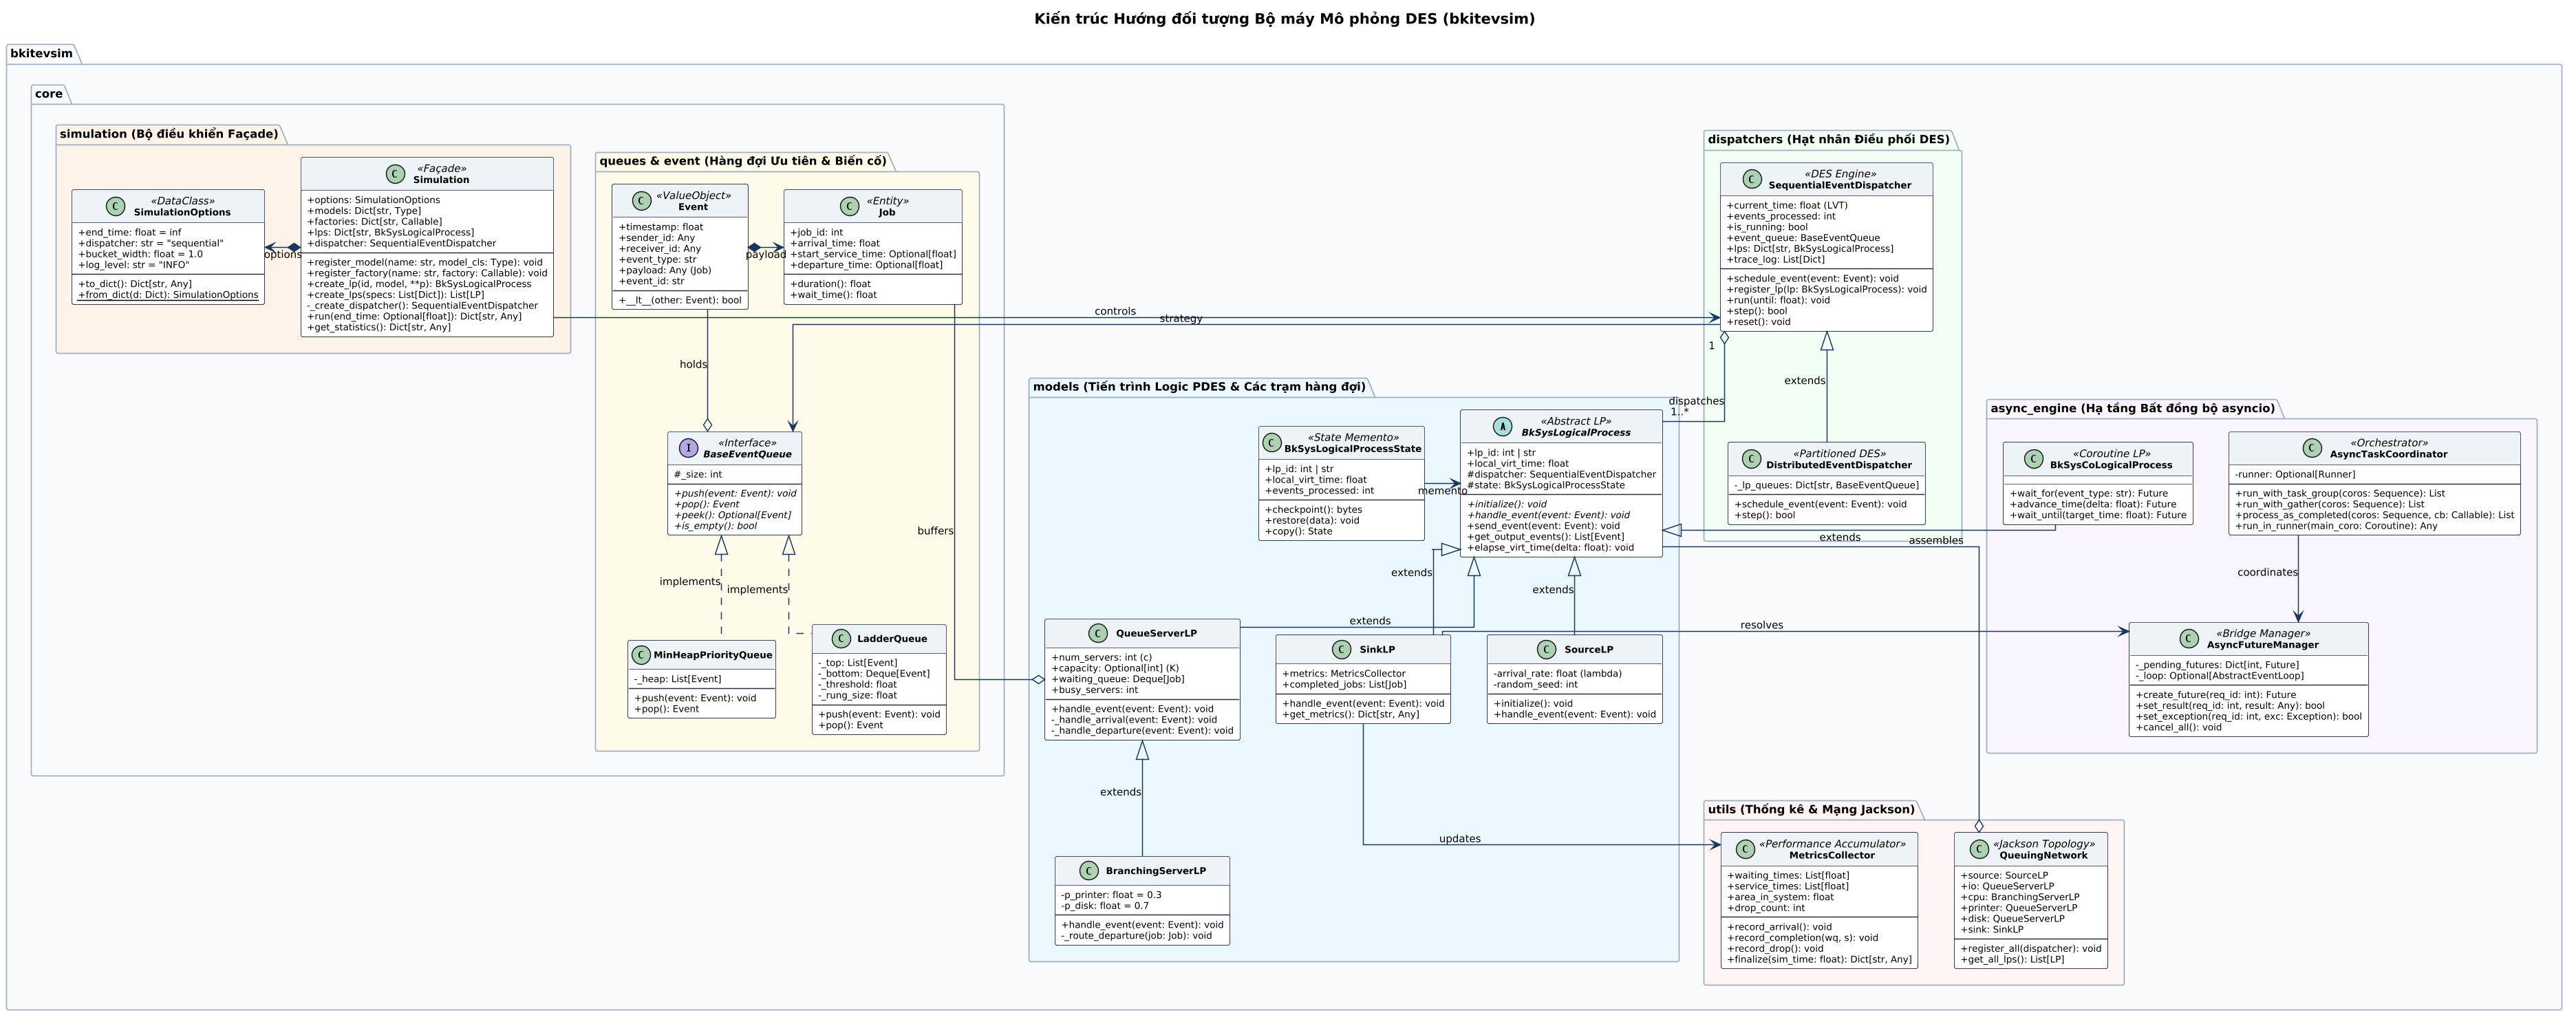
\includegraphics[width=0.98\textwidth]{image/uml_class_diagram.png}
\caption{Sơ đồ cấu trúc lớp chi tiết (UML Class Diagram) của hệ thống mô phỏng DES}
\label{fig:uml-class-diagram}
\end{figure}

\textbf{\large\hspace{0.5cm}Mô tả tổng quan sơ đồ lớp}

Sơ đồ lớp chi tiết tại Hình~\ref{fig:uml-class-diagram} đặc tả toàn diện kiến trúc hướng đối tượng của bộ máy mô phỏng sự kiện rời rạc kết hợp điều phối tác vụ bất đồng bộ (\textit{Discrete-Event Simulation with Asynchronous Task Coordination}). Hệ thống tổ chức phân tầng rõ rệt giữa bộ điều khiển Facade (\texttt{Simulation}, \texttt{SimulationOptions}), các dịch vụ điều phối sự kiện (\texttt{SequentialEventDispatcher}, \texttt{DistributedEventDispatcher}), cấu trúc hàng đợi ưu tiên (\texttt{BaseEventQueue}, \texttt{LadderQueue}), các trạm tiến trình logic PDES (\texttt{SourceLP}, \texttt{QueueServerLP}, \texttt{BranchingServerLP}, \texttt{SinkLP}) cùng hạ tầng quản lý tác vụ bất đồng bộ (\texttt{AsyncFutureManager}, \texttt{AsyncTaskCoordinator}) và thu thập số đo hiệu năng thời gian thực (\texttt{MetricsCollector}).

\textbf{\color{red}Phân hệ Điều khiển Mô phỏng Cấp cao (Simulation Controller Facade)}
\begin{itemize}[leftmargin=1.5em, itemsep=8pt]
\item \textbf{SimulationOptions}: Lớp đóng gói toàn diện các tham số cấu hình môi trường mô phỏng.

\begin{itemize}[leftmargin=1.2em, label={}, itemsep=3pt]
\item[\textendash] \textit{Thuộc tính:}
\begin{itemize}[leftmargin=1.5em, label=+, itemsep=2pt]
\item \texttt{end\_time: float} - Mốc thời gian ảo kết thúc mô phỏng (mặc định: 100.0).
\item \texttt{dispatcher: str} - Tên loại bộ điều phối (\texttt{"sequential"} hoặc \texttt{"distributed\_\allowbreak sequential"}).
\item \texttt{bucket\_width: float} - Bề rộng nấc thang $\Delta$ cho hàng đợi ưu tiên \texttt{LadderQueue}.
\item \texttt{log\_level: str} - Mức độ ghi nhật ký hệ thống (\texttt{"INFO"}, \texttt{"DEBUG"},...).
\item \texttt{log\_file: Optional[str]} - Đường dẫn tệp lưu trữ nhật ký ghi vết.
\item \texttt{stats\_file: Optional[str]} - Đường dẫn tệp xuất kết quả thống kê số liệu.
\item \texttt{verbose: bool} - Cờ bật/tắt chế độ in chi tiết tiến trình thực thi ra màn hình console.
\item \texttt{model\_params: Dict[str, Any]} - Từ điển chứa các tham số nghiệp vụ tùy biến bổ sung.
\end{itemize}

\item[\textendash] \textit{Phương thức:}
\begin{itemize}[leftmargin=1.5em, label=+, itemsep=2pt]
\item \texttt{to\_dict(): Dict[str, Any]} - Tuần tự hóa toàn bộ cấu hình sang đối tượng từ điển Python.
\item \texttt{from\_dict(data: Dict[str, Any]): SimulationOptions} - Phương thức lớp tái tạo đối tượng cấu hình từ dữ liệu từ điển/JSON.
\end{itemize}
\end{itemize}

\item \textbf{Simulation}: Lớp Facade mặt tiền điều phối cấp cao nhất, đóng vai trò là điểm chạm chính kết nối người dùng với bộ máy mô phỏng.

\begin{itemize}[leftmargin=1.2em, label={}, itemsep=3pt]
\item[\textendash] \textit{Thuộc tính:}
\begin{itemize}[leftmargin=1.5em, label=+, itemsep=2pt]
\item \texttt{options: SimulationOptions} - Đối tượng lưu trữ các cấu hình tham số vận hành.
\item \texttt{models: Dict[str, Type[BkSysLogicalProcess]]} - Danh bạ đăng ký các lớp mô hình logic theo tên.
\item \texttt{factories: Dict[str, Callable[..., BkSysLogicalProcess]]} - Danh bạ các hàm xưởng khởi tạo LP.
\item \texttt{lps: Dict[Any, BkSysLogicalProcess]} - Bảng băm quản lý toàn bộ thực thể tiến trình logic theo \texttt{lp\_id}.
\item \texttt{dispatcher: Optional[SequentialEventDispatcher]} - Con trỏ tham chiếu đến bộ điều phối đang hoạt động.
\end{itemize}

\item[\textendash] \textit{Phương thức:}
\begin{itemize}[leftmargin=1.5em, label=+, itemsep=2pt]
\item \texttt{register\_model(name, model\_cls)}: Đăng ký lớp mô hình \texttt{BkSysLogicalProcess} vào danh bạ.
\item \texttt{register\_factory(name: str, factory: Callable): void} - Đăng ký hàm xưởng khởi tạo LP tương ứng.
\item \texttt{create\_lp(lp\_id, model\_name, **params)}: Khởi tạo một thực thể LP theo mô hình đã đăng ký.
\item \texttt{create\_lps(model\_name, count, **params)}: Khởi tạo danh sách các thực thể LP cùng kiểu hàng loạt.
\item \texttt{get\_lp(lp\_id: int | str): Optional[BkSysLogicalProcess]} - Truy xuất thực thể LP theo mã định danh.
\item \texttt{get\_all\_lps(): List[BkSysLogicalProcess]} - Trả về danh sách tất cả các LP đã đăng ký.
\item \texttt{\_create\_dispatcher(): SequentialEventDispatcher} - Tự động khởi tạo bộ điều phối tuần tự hoặc phân vùng tương ứng với cấu hình.
\item \texttt{run(): Dict[str, Any]} - Khởi chạy kịch bản mô phỏng: liên kết toàn bộ LP vào Dispatcher, vận hành vòng lặp DES và trả về thống kê.
\item \texttt{get\_statistics(): Dict[str, Any]} - Thu gom và hợp nhất chỉ số thống kê từ Dispatcher và tất cả các trạm logic \texttt{per\_lp\_stats}.
\end{itemize}
\end{itemize}
\end{itemize}

\textbf{\color{red}Phân hệ Hạt nhân \& Điều phối sự kiện}
\begin{itemize}[leftmargin=1.5em, itemsep=8pt]
\item \textbf{SequentialEventDispatcher (alias Dispatcher)}: Hạt nhân điều hành trung tâm quản lý vòng đời sự kiện theo thứ tự mốc thời gian ảo đơn điệu.

\begin{itemize}[leftmargin=1.2em, label={}, itemsep=3pt]
\item[\textendash] \textit{Thuộc tính:}
\begin{itemize}[leftmargin=1.5em, label=+, itemsep=2pt]
\item \texttt{end\_time: float} - Mốc thời gian ảo chặn trên để kết thúc mô phỏng.
\item \texttt{bucket\_width: float} - Bề rộng nấc thang của hàng đợi \texttt{LadderQueue}.
\item \texttt{lps: Dict[Any, BkSysLogicalProcess]} - Bảng tra cứu danh bạ các tiến trình logic theo \texttt{lp\_id}.
\item \texttt{event\_queue: BaseEventQueue} - Hàng đợi sự kiện ưu tiên (\texttt{LadderQueue} hoặc \texttt{MinHeapPriorityQueue}).
\item \texttt{current\_time: float} - Mốc thời gian ảo hiện tại của hệ thống ($LVT$ toàn cục).
\item \texttt{events\_processed: int} - Tổng số sự kiện đã được trích xuất và xử lý thành công.
\item \texttt{trace\_log: List[Dict[str, Any]]} - Nhật ký ghi vết kiểm tra tính đơn điệu nhân quả ($t_{k+1} \ge t_k$).
\item \texttt{max\_trace\_entries: int} - Giới hạn dung lượng bộ nhớ nhật ký vết (mặc định 1000).
\item \texttt{stats: Dict[str, Any]} - Báo cáo thống kê thời gian ảo và thời gian thực máy tính.
\item \texttt{\_initialized: bool} - Cờ trạng thái bảo đảm quy trình mồi sự kiện ban đầu \texttt{initialize()} chỉ chạy 1 lần.
\end{itemize}

\item[\textendash] \textit{Phương thức:}
\begin{itemize}[leftmargin=1.5em, label=+, itemsep=2pt]
\item \texttt{register\_lp(lp: BkSysLogicalProcess): void} - Đăng ký tiến trình logic vào danh bạ và liên kết Dispatcher.
\item \texttt{get\_lp(lp\_id: Any): Optional[BkSysLogicalProcess]} - Tra cứu trạm logic theo định danh.
\item \texttt{get\_all\_lps(): List[BkSysLogicalProcess]} - Lấy toàn bộ danh sách trạm logic đã đăng ký.
\item \texttt{schedule\_event(event: Event): void} - Đẩy sự kiện mới vào hàng đợi sự kiện ưu tiên.
\item \texttt{schedule\_initial\_events(): void} - Duyệt toàn bộ LPs và kích hoạt phương thức \texttt{initialize()} mồi sự kiện đầu tiên.
\item \texttt{run(end\_time: Optional[float]): Dict[str, Any]} - Thực thi vòng lặp DES chính cho đến khi đạt \texttt{end\_time} hoặc hàng đợi rỗng.
\end{itemize}
\end{itemize}

\item \textbf{DistributedEventDispatcher}: Kế thừa từ \texttt{SequentialEventDispatcher}, hiện thực mô hình phân vùng hàng đợi cục bộ (\textit{Partitioned Queues}).

\begin{itemize}[leftmargin=1.2em, label={}, itemsep=3pt]
\item[\textendash] \textit{Thuộc tính:}
\begin{itemize}[leftmargin=1.5em, label=+, itemsep=2pt]
\item \texttt{\_lp\_queues: Dict[Any, LadderQueue]} - Bảng ánh xạ mỗi LP tới một hàng đợi \texttt{LadderQueue} cục bộ độc lập.
\end{itemize}

\item[\textendash] \textit{Phương thức:}
\begin{itemize}[leftmargin=1.5em, label=+, itemsep=2pt]
\item \texttt{register\_lp(lp: BkSysLogicalProcess): void} - Đăng ký LP và cấp phát một hàng đợi \texttt{LadderQueue} riêng biệt.
\item \texttt{schedule\_event(event: Event): void} - Định tuyến sự kiện trực tiếp vào hàng đợi cục bộ của trạm đích \texttt{receiver\_id}.
\item \texttt{run(end\_time: Optional[float]): Dict[str, Any]} - Tại mỗi bước lặp, quét tìm LP có sự kiện sớm nhất trên toàn mạng để trích xuất và xử lý.
\end{itemize}
\end{itemize}

\item \textbf{Event}: Đối tượng giá trị (\textit{Value Object}) đóng gói thông điệp và ngữ cảnh trao đổi giữa các thành phần mô phỏng.

\begin{itemize}[leftmargin=1.2em, label={}, itemsep=3pt]
\item[\textendash] \textit{Thuộc tính:}
\begin{itemize}[leftmargin=1.5em, label=+, itemsep=2pt]
\item \texttt{timestamp: float} - Mốc thời gian ảo kích hoạt sự kiện (tiêu chí so sánh tự nhiên duy nhất).
\item \texttt{sender\_id: Any} (alias \texttt{source\_lp}, \texttt{lp\_source}) - Định danh trạm logic phát sự kiện (\texttt{compare=False}).
\item \texttt{receiver\_id: Any} (alias \texttt{dest\_lp}, \texttt{lp\_target}) - Định danh trạm logic tiếp nhận sự kiện (\texttt{compare=False}).
\item \texttt{event\_type: Any} - Kiểu sự kiện (\texttt{ARRIVAL}, \texttt{SERVICE\_START}, \texttt{DEPARTURE}, \texttt{TERMINATE}) (\texttt{compare=False}).
\item \texttt{payload: Any} (alias \texttt{data}) - Tải trọng dữ liệu đi kèm (thường chứa thực thể \texttt{Job}) (\texttt{compare=False}).
\item \texttt{event\_id: Any} - Mã định danh duy nhất của sự kiện dạng UUID4 tự sinh (\texttt{compare=False}).
\item \texttt{\_priority: int} - Giá trị độ ưu tiên nghiệp vụ mặc định phục vụ tương thích ngược.
\end{itemize}

\item[\textendash] \textit{Phương thức:}
\begin{itemize}[leftmargin=1.5em, label=+, itemsep=2pt]
\item \texttt{\_\_lt\_\_(other: Event): bool} - So sánh thứ tự ưu tiên trích xuất dựa trên mốc thời gian ảo \texttt{timestamp} (\texttt{@dataclass(order=True)}).
\end{itemize}
\end{itemize}

\item \textbf{Job}: Thực thể đại diện cho một tác vụ, khách hàng hoặc gói tin luân chuyển trong mạng hàng đợi.

\begin{itemize}[leftmargin=1.2em, label={}, itemsep=3pt]
\item[\textendash] \textit{Thuộc tính:}
\begin{itemize}[leftmargin=1.5em, label=+, itemsep=2pt]
\item \texttt{job\_id: int} - Mã định danh duy nhất của yêu cầu trong toàn bộ kịch bản.
\item \texttt{orig\_arrival\_time: float} - Mốc thời gian ảo yêu cầu gia nhập mạng lần đầu tiên (phục vụ tính trễ toàn trình).
\item \texttt{arrival\_time: float} - Mốc thời gian ảo yêu cầu xuất hiện tại trạm logic hiện tại.
\item \texttt{start\_service\_time: Optional[float]} - Thời điểm yêu cầu bắt đầu được máy chủ xử lý.
\item \texttt{departure\_time: Optional[float]} - Thời điểm yêu cầu hoàn tất và rời khỏi trạm.
\end{itemize}
\end{itemize}
\end{itemize}

\textbf{\color{red}Phân hệ Quản lý Hàng đợi Ưu tiên}

\begin{itemize}[leftmargin=1.5em, itemsep=8pt]
\item \textbf{BaseEventQueue}: Là giao diện trừu tượng (\textit{Interface/Abstract Base Class}) định nghĩa hợp đồng chung cho các cấu trúc hàng đợi sự kiện.

\begin{itemize}[leftmargin=1.2em, label={}, itemsep=3pt]
\item[\textendash] \textit{Phương thức:}
\begin{itemize}[leftmargin=1.5em, label=+, itemsep=2pt]
\item \texttt{push(event: Event): void} - Thêm một sự kiện mới vào cấu trúc hàng đợi.
\item \texttt{pop(): Event} - Trích xuất và loại bỏ sự kiện có mốc thời gian ảo nhỏ nhất.
\item \texttt{peek(): Optional[Event]} - Xem sự kiện sớm nhất ở đầu hàng mà không loại bỏ.
\item \texttt{is\_empty(): bool} - Kiểm tra xem hàng đợi có rỗng hay không.
\item \texttt{\_\_len\_\_(): int} - Trả về kích thước hiện tại của hàng đợi.
\end{itemize}
\end{itemize}

\item \textbf{MinHeapPriorityQueue}: Hiện thực cây nhị phân Min-Heap chuẩn dựa trên module \texttt{heapq} với chi phí thời gian $\mathcal{O}(\log N)$, phù hợp cho các kịch bản thực nghiệm quy mô vừa và nhỏ.

\begin{itemize}[leftmargin=1.2em, label={}, itemsep=3pt]
\item[\textendash] \textit{Thuộc tính:}
\begin{itemize}[leftmargin=1.5em, label=+, itemsep=2pt]
\item \texttt{\_heap: List[Event]} - Mảng lưu trữ các nút cây nhị phân heap theo mốc thời gian.
\end{itemize}

\item[\textendash] \textit{Phương thức:}
\begin{itemize}[leftmargin=1.5em, label=+, itemsep=2pt]
\item \texttt{push(event: Event): void} - Đẩy sự kiện vào heap qua thao tác \texttt{heappush}.
\item \texttt{pop(): Event} - Lấy phần tử gốc có timestamp nhỏ nhất qua \texttt{heappop}.
\item \texttt{peek(): Optional[Event]} - Trả về phần tử tại vị trí gốc \texttt{\_heap[0]}.
\item \texttt{is\_empty(): bool} - Kiểm tra danh sách \texttt{\_heap} có rỗng hay không.
\end{itemize}
\end{itemize}

\item \textbf{LadderQueue}: Hiện thực thuật toán hàng đợi phân tầng hai cấp (\texttt{\_bottom} và \texttt{\_top}) theo Hình 3 đề bài, tối ưu hóa chi phí trích xuất trung bình đạt $\mathcal{O}(1)$ cho các kịch bản tải bùng nổ lên đến hàng triệu sự kiện.

\begin{itemize}[leftmargin=1.2em, label={}, itemsep=3pt]
\item[\textendash] \textit{Thuộc tính:}
\begin{itemize}[leftmargin=1.5em, label=+, itemsep=2pt]
\item \texttt{bucket\_width: float} (alias \texttt{rung\_width}) - Bề rộng nấc thang thời gian phục vụ việc hạ sự kiện.
\item \texttt{\_bottom: List[Event]} - Hàng đợi Min-Heap nhỏ chứa các sự kiện cận kề ($t \le \text{\_boundary}$).
\item \texttt{\_top: List[Event]} - Hàng đợi Min-Heap chứa các sự kiện xa trong tương lai ($t > \text{\_boundary}$).
\item \texttt{\_boundary: float} - Mốc thời gian ảo phân tầng giữa tầng đáy và tầng đỉnh.
\item \texttt{\_count: int} - Tổng số lượng sự kiện đang lưu giữ trong cấu trúc.
\end{itemize}

\item[\textendash] \textit{Phương thức:}
\begin{itemize}[leftmargin=1.5em, label=+, itemsep=2pt]
\item \texttt{push(event: Event): void} - Đặt sự kiện vào \texttt{\_bottom} nếu $t \le \text{\_boundary}$, ngược lại vào \texttt{\_top}.
\item \texttt{pop(): Event} - Rút sự kiện từ \texttt{\_bottom}; nếu rỗng thì kích hoạt \texttt{\_refill\_bottom()}.
\item \texttt{peek(): Optional[Event]} - Xem sự kiện sớm nhất ở đầu \texttt{\_bottom} hoặc đỉnh \texttt{\_top}.
\item \texttt{\_refill\_bottom(): void} - Hạ một nấc thang sự kiện từ \texttt{\_top} xuống \texttt{\_bottom} và cập nhật \texttt{\_boundary}.
\end{itemize}
\end{itemize}
\end{itemize}

\textbf{\color{red}Phân hệ Tiến trình Logic PDES}

\begin{itemize}[leftmargin=1.5em, itemsep=8pt]
\item \textbf{BkSysLogicalProcessState}: Lớp bao đóng trạng thái khả biến của tiến trình logic, hỗ trợ chụp ảnh nhanh và lưu vết.

\begin{itemize}[leftmargin=1.2em, label={}, itemsep=3pt]
\item[\textendash] \textit{Thuộc tính:}
\begin{itemize}[leftmargin=1.5em, label=+, itemsep=2pt]
\item \texttt{\_data: Dict[str, Any]} - Từ điển lưu trữ các biến trạng thái nội tại.
\item \texttt{history: List[Dict[str, Any]]} - Lịch sử các bước chuyển dịch trạng thái theo thời gian ảo.
\end{itemize}

\item[\textendash] \textit{Phương thức:}
\begin{itemize}[leftmargin=1.5em, label=+, itemsep=2pt]
\item \texttt{get(key, default): Any} / \texttt{set(key, value): void} - Đọc và ghi biến trạng thái.
\item \texttt{checkpoint(): Dict[str, Any]} - Sao chép sâu (\textit{Deep-copy}) toàn bộ trạng thái tại mốc kiểm tra.
\item \texttt{restore(checkpoint): void} - Khôi phục trạng thái từ bản chụp nhanh.
\item \texttt{record\_step(timestamp, description, data): void} - Ghi nhận bước chuyển dịch trạng thái phục vụ debug.
\end{itemize}
\end{itemize}

\item \textbf{BkSysLogicalProcess (alias LogicalProcess)}: Lớp cơ sở trừu tượng cho mọi thực thể mô phỏng PDES.

\begin{itemize}[leftmargin=1.2em, label={}, itemsep=3pt]
\item[\textendash] \textit{Thuộc tính:}
\begin{itemize}[leftmargin=1.5em, label=+, itemsep=2pt]
\item \texttt{lp\_id: int | str} - Mã định danh duy nhất của tiến trình logic.
\item \texttt{local\_virt\_time: float} (alias \texttt{local\_virtual\_time}) - Đồng hồ ảo cục bộ ($LVT$) của trạm.
\item \texttt{state: BkSysLogicalProcessState} - Thực thể trạng thái nội tại của trạm.
\item \texttt{\_output\_events: List[Event]} - Danh sách vùng đệm chứa các sự kiện chuẩn bị xuất xưởng.
\item \texttt{\_dispatcher: Optional[Any]} - Tham chiếu ngược đến bộ điều phối sự kiện.
\item \texttt{\_handlers: Dict[str, Callable]} - Bảng tra cứu hàm xử lý nghiệp vụ theo loại sự kiện.
\end{itemize}

\item[\textendash] \textit{Phương thức:}
\begin{itemize}[leftmargin=1.5em, label=+, itemsep=2pt]
\item \texttt{initialize(): void} / \texttt{finalize(): void} - Hook khởi tạo và chốt sổ vòng đời trạm logic.
\item \texttt{get\_local\_virt\_time(): float} - Lấy mốc thời gian ảo cục bộ hiện tại.
\item \texttt{set\_local\_virt\_time(t: float): void} - Cập nhật $LVT$, kiểm soát nghiêm ngặt ràng buộc nhân quả LCC ($t \ge LVT$).
\item \texttt{elapse\_virt\_time(delta: float): float} - Tịnh tiến $LVT$ thêm một khoảng trễ $\Delta t \ge 0$.
\item \texttt{register\_handler(event\_type, handler): void} - Đăng ký hàm callback xử lý theo loại sự kiện.
\item \texttt{send\_event(event: Event): void} - Gửi bản tin sự kiện tới trạm khác hoặc đẩy vào bộ điều phối.
\item \texttt{get\_output\_events(): List[Event]} - Trích xuất và dọn sạch danh sách sự kiện xuất xưởng.
\item \texttt{handle\_event(event: Event): void} - Tiếp nhận và kích hoạt xử lý biến cố.
\item \texttt{reset(): void} - Tái lập đồng hồ $LVT$ và hàng đợi xuất xưởng về trạng thái khởi đầu.
\end{itemize}
\end{itemize}

\item \textbf{SourceLP}: Tiến trình nguồn chịu trách nhiệm tự phát sinh dòng yêu cầu Poisson ngoại vi vào hệ thống.

\begin{itemize}[leftmargin=1.2em, label={}, itemsep=3pt]
\item[\textendash] \textit{Thuộc tính:}
\begin{itemize}[leftmargin=1.5em, label=+, itemsep=2pt]
\item \texttt{dest\_lp\_id: int | str} - Định danh trạm tiếp nhận kế tiếp (mặc định: \texttt{"Server"}).
\item \texttt{arrival\_rate: float} - Tốc độ phát sinh yêu cầu trung bình $\lambda$ (yêu cầu/giây).
\item \texttt{burst\_prob: float} / \texttt{burst\_size: int} - Xác suất và kích thước chùm sự kiện tải bùng nổ.
\item \texttt{\_job\_counter: int} - Bộ đếm tổng số yêu cầu đã sinh ra từ đầu kịch bản.
\item \texttt{\_started: bool} - Cờ chống phát sinh trùng lặp sự kiện mồi đầu tiên.
\end{itemize}

\item[\textendash] \textit{Phương thức:}
\begin{itemize}[leftmargin=1.5em, label=+, itemsep=2pt]
\item \texttt{initialize(): void} / \texttt{start(): void} - Kích hoạt tự lên lịch sự kiện đến đầu tiên $\Delta t \sim \text{Exp}(\lambda)$.
\item \texttt{handle\_event(event: Event): void} - Đóng gói thực thể \texttt{Job}, chuyển tiếp sang trạm sau và tự lên lịch khách kế tiếp.
\end{itemize}
\end{itemize}

\item \textbf{QueueServerLP}: Trạm phục vụ tích hợp hàng đợi và cụm máy chủ song song theo chuẩn Kendall $A/S/c/K$.

\begin{itemize}[leftmargin=1.2em, label={}, itemsep=3pt]
\item[\textendash] \textit{Thuộc tính:}
\begin{itemize}[leftmargin=1.5em, label=+, itemsep=2pt]
\item \texttt{dest\_lp\_id: int | str} - Định danh trạm tiếp nhận kế tiếp (mặc định: \texttt{"Sink"}).
\item \texttt{service\_rate: float} - Năng lực phục vụ của mỗi máy chủ $\mu$ (yêu cầu/giây).
\item \texttt{num\_servers: float} - Số lượng máy chủ song song $c$ ($1 \le c \le \infty$).
\item \texttt{capacity: Optional[int]} - Sức chứa tối đa của hệ thống $K$ ($K = \text{None}$ nếu đệm vô hạn).
\item \texttt{metrics: MetricsCollector} - Bộ tích lũy mẫu đo hiệu năng tích hợp sẵn tại trạm.
\item \texttt{waiting\_queue: Deque[Job]} - Hàng ghế chờ FIFO lưu giữ các yêu cầu đang đợi máy chủ rảnh.
\item \texttt{busy\_servers: int} - Số lượng máy chủ đang bận xử lý tại mốc giờ ảo hiện tại.
\item \texttt{total\_in\_system: int} (property) - Tổng số khách đang có mặt trong trạm ($\text{busy} + |\text{queue}|$).
\end{itemize}

\item[\textendash] \textit{Phương thức:}
\begin{itemize}[leftmargin=1.5em, label=+, itemsep=2pt]
\item \texttt{handle\_event(event: Event): void} - Phân luồng sự kiện \texttt{ARRIVAL} hoặc \texttt{DEPARTURE}.
\item \texttt{\_handle\_arrival(event: Event): void} - Kiểm tra tràn đệm $K$, loại bỏ gói tin nếu đầy, phân bổ server rảnh hoặc xếp hàng.
\item \texttt{\_start\_service(job: Job, current\_time: float): void} - Đặt mốc bắt đầu phục vụ, bốc thời gian phục vụ $S \sim \text{Exp}(\mu)$ và lên lịch hoàn tất.
\item \texttt{\_handle\_departure(event: Event): void} - Ghi nhận số đo hoàn tất, chuyển Job sang trạm sau và đón khách kế tiếp từ hàng đợi.
\item \texttt{\_notify\_state(current\_time: float): void} - Cập nhật trạng thái tích phân diện tích theo thời gian.
\item \texttt{finalize(): void} / \texttt{get\_metrics(): Dict[str, Any]} - Chốt sổ và trích xuất vector chỉ số hiệu năng.
\end{itemize}
\end{itemize}

\item \textbf{BranchingServerLP}: Kế thừa từ \texttt{QueueServerLP}, chuyên biệt hóa cơ chế rẽ nhánh ngẫu nhiên Bernoulli cho mạng hàng đợi Jackson.

\begin{itemize}[leftmargin=1.2em, label={}, itemsep=3pt]
\item[\textendash] \textit{Thuộc tính:}
\begin{itemize}[leftmargin=1.5em, label=+, itemsep=2pt]
\item \texttt{printer\_lp\_id: int | str} / \texttt{disk\_lp\_id: int | str} - Định danh trạm Máy in và Ổ đĩa.
\item \texttt{p\_printer: float} - Xác suất rẽ nhánh tới Máy in ($p = 0.3$, còn lại $1-p = 0.7$ tới Ổ đĩa).
\end{itemize}

\item[\textendash] \textit{Phương thức:}
\begin{itemize}[leftmargin=1.5em, label=+, itemsep=2pt]
\item \texttt{\_handle\_departure(event: Event): void} - Ghi đè xử lý hoàn tất để thực hiện phép thử Bernoulli định tuyến ngẫu nhiên.
\end{itemize}
\end{itemize}

\item \textbf{SinkLP}: Điểm thu gom cuối cùng của dòng xử lý, tính toán độ trễ toàn trình và giải phóng các lời hứa bất đồng bộ.

\begin{itemize}[leftmargin=1.2em, label={}, itemsep=3pt]
\item[\textendash] \textit{Thuộc tính:}
\begin{itemize}[leftmargin=1.5em, label=+, itemsep=2pt]
\item \texttt{future\_manager: Optional[Any]} - Cầu nối giải phóng Future cho phía ứng dụng coroutine.
\item \texttt{completed\_jobs: List[Job]} - Danh sách toàn bộ các thực thể \texttt{Job} đã hoàn tất.
\item \texttt{total\_response\_times: List[float]} - Danh sách mảng thời gian lưu trú toàn trình của từng yêu cầu.
\item \texttt{total\_completed: int} (property) - Đếm tổng số yêu cầu đã hoàn tất.
\end{itemize}

\item[\textendash] \textit{Phương thức:}
\begin{itemize}[leftmargin=1.5em, label=+, itemsep=2pt]
\item \texttt{handle\_event(event: Event): void} - Ghi nhận thời gian lưu trú $W = t_{\text{dep}} - t_{\text{orig\_arr}}$ và kích hoạt \texttt{set\_result()} cho Future tương ứng.
\item \texttt{get\_metrics(): Dict[str, Any]} - Tính toán thời gian phản hồi trung bình và tổng số yêu cầu hoàn thành.
\end{itemize}
\end{itemize}

\item \textbf{NetworkSinkLP}: Kế thừa từ \texttt{SinkLP}, chuyên biệt hóa tính toán độ trễ toàn trình cho mạng đa chặng Jackson.

\begin{itemize}[leftmargin=1.2em, label={}, itemsep=3pt]
\item[\textendash] \textit{Thuộc tính:}
\begin{itemize}[leftmargin=1.5em, label=+, itemsep=2pt]
\item \texttt{network\_latencies: List[float]} - Mảng lưu trữ thời gian trễ toàn trình mạng từ trạm nguồn đến trạm đích.
\end{itemize}

\item[\textendash] \textit{Phương thức:}
\begin{itemize}[leftmargin=1.5em, label=+, itemsep=2pt]
\item \texttt{handle\_event(event: Event): void} - Ghi nhận thời gian trễ $T = t_{\text{Sink}} - \text{job.orig\_arrival\_time}$.
\item \texttt{get\_metrics(): Dict[str, Any]} - Xuất chỉ số độ trễ mạng trung bình \texttt{mean\_network\_latency}.
\end{itemize}
\end{itemize}

\item \textbf{QueuingNetwork}: Lớp hỗ trợ đóng gói cấu hình và kết nối mạng hàng đợi 4 trạm máy tính (Hình 1 đề bài).

\begin{itemize}[leftmargin=1.2em, label={}, itemsep=3pt]
\item[\textendash] \textit{Thuộc tính:}
\begin{itemize}[leftmargin=1.5em, label=+, itemsep=2pt]
\item \texttt{source: SourceLP}, \texttt{io: QueueServerLP}, \texttt{cpu: BranchingServerLP}.
\item \texttt{printer: QueueServerLP}, \texttt{disk: QueueServerLP}, \texttt{sink: NetworkSinkLP}.
\end{itemize}

\item[\textendash] \textit{Phương thức:}
\begin{itemize}[leftmargin=1.5em, label=+, itemsep=2pt]
\item \texttt{register\_all(dispatcher: Any): void} - Tự động nạp toàn bộ 6 trạm mạng vào bộ điều phối.
\end{itemize}
\end{itemize}
\end{itemize}

\textbf{\color{red}Phân hệ Cầu nối Bất đồng bộ \& Thu thập Dữ liệu}

\begin{itemize}[leftmargin=1.5em, itemsep=8pt]
\item \textbf{AsyncFutureManager}: Cầu nối phi nghẽn giữa môi trường mô phỏng thời gian ảo và cơ chế \texttt{asyncio.Future} của Python.

\begin{itemize}[leftmargin=1.2em, label={}, itemsep=3pt]
\item[\textendash] \textit{Thuộc tính:}
\begin{itemize}[leftmargin=1.5em, label=+, itemsep=2pt]
\item \texttt{loop: Optional[asyncio.AbstractEventLoop]} - Vòng lặp sự kiện bất đồng bộ thực tế.
\item \texttt{\_pending\_futures: Dict[int, asyncio.Future]} - Bản đồ lưu trữ các Future đang chờ xử lý theo \texttt{request\_id}.
\end{itemize}

\item[\textendash] \textit{Phương thức:}
\begin{itemize}[leftmargin=1.5em, label=+, itemsep=2pt]
\item \texttt{\_get\_loop(): asyncio.AbstractEventLoop} - Lấy Event Loop đang chạy hoặc tạo mới an toàn trên Python 3.10+.
\item \texttt{create\_future(request\_id: int): asyncio.Future} - Tạo mới một lời hứa Future gắn với \texttt{request\_id} và trao cho người dùng \texttt{await}.
\item \texttt{set\_result(request\_id: int, result: Any): bool} - Gán kết quả hoàn tất cho Future, đánh thức coroutine tương ứng mà không phong tỏa luồng điều phối.
\item \texttt{set\_exception(request\_id: int, exception: Exception): bool} - Báo lỗi vào Future khi gặp sự cố.
\item \texttt{cancel\_all(): void} - Hủy bỏ toàn bộ Future đang treo khi dừng hệ thống.
\item \texttt{has\_pending(request\_id: int): bool} / \texttt{pending\_count(): int} - Kiểm tra số lượng yêu cầu đang chờ giải phóng.
\end{itemize}
\end{itemize}

\item \textbf{AsyncTaskCoordinator}: Hiện thực các mẫu phối hợp tác vụ đồng quy chuẩn hóa của Python \texttt{asyncio}.

\begin{itemize}[leftmargin=1.2em, label={}, itemsep=3pt]
\item[\textendash] \textit{Phương thức tĩnh:}
\begin{itemize}[leftmargin=1.5em, label=+, itemsep=2pt]
\item \texttt{run\_with\_task\_group(coroutines: Sequence): List[Any]} - Quản lý tác vụ cấu trúc (\textit{Structured Concurrency}) qua \texttt{asyncio.TaskGroup}.
\item \texttt{run\_with\_gather(coroutines: Sequence): List[Any]} - Thu gom kết quả song song hàng loạt qua \texttt{asyncio.gather}.
\item \texttt{process\_as\_completed(coroutines, callback)}: Trả về kết quả ngay khi từng tác vụ riêng lẻ hoàn tất theo nguyên tắc FCFS qua \texttt{asyncio.as\_completed}.
\item \texttt{run\_in\_runner(main\_coro: Coroutine): Any} - Điểm khởi động chương trình với bộ thực thi \texttt{asyncio.Runner} cô lập.
\end{itemize}
\end{itemize}

\item \textbf{BkSysCoLogicalProcess \& BkSysFuture}: Động cơ PDES hướng Coroutine hỗ trợ cú pháp \texttt{async/await} bản địa.

\begin{itemize}[leftmargin=1.2em, label={}, itemsep=3pt]
\item[\textendash] \textit{Thuộc tính \& Phương thức:}
\begin{itemize}[leftmargin=1.5em, label=+, itemsep=2pt]
\item \texttt{await self.wait\_for(event\_type: str): Event} - Tạm dừng coroutine cho đến khi bản tin sự kiện phù hợp xuất hiện.
\item \texttt{await self.advance\_time(delta: float): float} - Tịnh tiến thời gian ảo cục bộ phi nghẽn luồng.
\item \texttt{BkSysFuture}: Kế thừa từ \texttt{asyncio.Future}, cung cấp các kiểm tra trạng thái (\texttt{is\_pending}, \texttt{is\_resolved}, \texttt{is\_rejected}) và hook callback xử lý lỗi.
\end{itemize}
\end{itemize}

\item \textbf{MetricsCollector}: Bộ tích lũy mẫu đo hiệu năng và tính tích phân thời gian thực.

\begin{itemize}[leftmargin=1.2em, label={}, itemsep=3pt]
\item[\textendash] \textit{Thuộc tính:}
\begin{itemize}[leftmargin=1.5em, label=+, itemsep=2pt]
\item \texttt{arrived\_count: int} / \texttt{completed\_count: int} / \texttt{dropped\_count: int} - Bộ đếm số khách đến, hoàn tất và bị loại bỏ do tràn đệm.
\item \texttt{waiting\_times: List[float]} / \texttt{service\_times: List[float]} / \texttt{response\_times: List[float]} - Mảng lưu trữ thời gian chờ, phục vụ và lưu trú.
\item \texttt{\_area\_q\_len: float} / \texttt{\_area\_in\_sys: float} / \texttt{\_area\_busy\_servers: float} - Tích lũy diện tích hình chữ nhật tích phân thời gian $\sum \text{State} \cdot \Delta t$.
\end{itemize}

\item[\textendash] \textit{Phương thức:}
\begin{itemize}[leftmargin=1.5em, label=+, itemsep=2pt]
\item \texttt{update\_state(current\_time, q\_len, in\_sys, busy\_servers): void} - Cập nhật diện tích tích phân theo bước nhảy thời gian thực $\Delta t$.
\item \texttt{record\_arrival(): void} / \texttt{record\_drop(): void} - Ghi nhận lượt đến và rớt gói do quá tải $K$.
\item \texttt{record\_completion(wait\_time, serv\_time): void} - Ghi nhận mẫu thời gian khi hoàn tất phục vụ.
\item \texttt{finalize(total\_sim\_time, num\_servers): Dict[str, float]} - Tính toán toàn bộ chỉ số hiệu năng chuẩn: $W, W_q, S, L, L_q, \rho, P_b, \lambda_{\text{eff}}$.
\end{itemize}
\end{itemize}
\end{itemize}

\subsubsection{Mối quan hệ giữa các lớp trong hệ thống}
\label{subsubsec:uml-class-relationships}

\hspace{0.5cm}Các thành phần đối tượng phối hợp chặt chẽ với nhau thông qua các cơ chế điều phối thời gian ảo, luân chuyển thông điệp sự kiện và giải phóng lời hứa bất đồng bộ:

\begin{itemize}[leftmargin=1.5em, itemsep=4pt]
\item \textbf{Quan hệ Điều khiển Facade cấp cao (\textit{Facade Orchestration}):} Lớp mặt tiền \texttt{Simulation} đóng vai trò là nhạc trưởng cấp cao nhất, kết tập (\textit{Aggregation}) đối tượng cấu hình \texttt{SimulationOptions}, quản lý khởi tạo hạt nhân điều phối \texttt{SequentialEventDispatcher} (hoặc mô hình phân vùng \texttt{DistributedEventDispatcher}) và sở hữu danh bạ tập hợp các thực thể \texttt{BkSysLogicalProcess}. Nhờ đó, ứng dụng người dùng chỉ cần giao tiếp qua giao diện duy nhất của Facade mà không phải can thiệp thủ công vào các tầng bên dưới.
\item \textbf{Quan hệ Quản lý \& Điều phối (Management):} \texttt{SequentialEventDispatcher} nắm giữ một tham chiếu duy nhất tới giao diện \texttt{BaseEventQueue} theo mẫu thiết kế \textit{Strategy Pattern}, cho phép hoán đổi cấu trúc hàng đợi linh hoạt tại thời điểm chạy. Đồng thời, \texttt{SequentialEventDispatcher} quản lý danh bạ kết tập gồm nhiều \texttt{BkSysLogicalProcess} để chuyển giao sự kiện qua phương thức \texttt{handle\_event()}.
\item \textbf{Quan hệ Kế thừa (Inheritance):} 
\begin{itemize}[leftmargin=1.2em, itemsep=2pt]
\item \texttt{MinHeapPriorityQueue} và \texttt{LadderQueue} kế thừa và hiện thực các phương thức trừu tượng của \texttt{BaseEventQueue}.
\item \texttt{SourceLP}, \texttt{QueueServerLP} và \texttt{SinkLP} cùng kế thừa từ lớp cơ sở \texttt{LogicalProcess}, thừa hưởng đồng hồ ảo $LVT$ và năng lực \texttt{send\_event()}.
\item \texttt{BranchingServerLP} chuyên biệt hóa từ \texttt{QueueServerLP}, tái sử dụng toàn bộ hàng đợi $c$ máy chủ và chỉ ghi đè logic rẽ nhánh ngẫu nhiên.
\end{itemize}
\item \textbf{Quan hệ Sở hữu \& Đóng gói (Composition / Aggregation):} \texttt{Event} đóng gói thực thể \texttt{Job} trong trường \texttt{payload}. \texttt{QueueServerLP} sở hữu hàng ghế chờ FIFO \texttt{waiting\_queue} kiểu \texttt{deque[Job]}. \texttt{SinkLP} kết tập đối tượng \texttt{MetricsCollector} để tích lũy dữ liệu.
\item \textbf{Quan hệ Cầu nối Bất đồng bộ (Async Bridging):} Khi một yêu cầu hoàn tất tại trạm cuối, \texttt{SinkLP} kích hoạt phương thức \texttt{set\_result()} trên \texttt{AsyncFutureManager}, đánh thức coroutine phía người dùng mà không làm nghẽn tiến trình mô phỏng rời rạc.
\item \textbf{Cơ chế Tuân thủ 5 Nguyên tắc SOLID:} Đảm bảo tính mở rộng cao: khi cần bổ sung một kỷ luật phục vụ mới hay một thuật toán hàng đợi mới, chỉ cần mở rộng lớp tương ứng mà không phải can thiệp vào hạt nhân điều phối \texttt{Dispatcher}.
\end{itemize}


\newpage
\subsubsection{Sơ đồ tuần tự tương tác sự kiện (UML Sequence Diagram)}
\label{subsubsec:uml-sequence-diagram}
\begin{figure}[H]
\centering
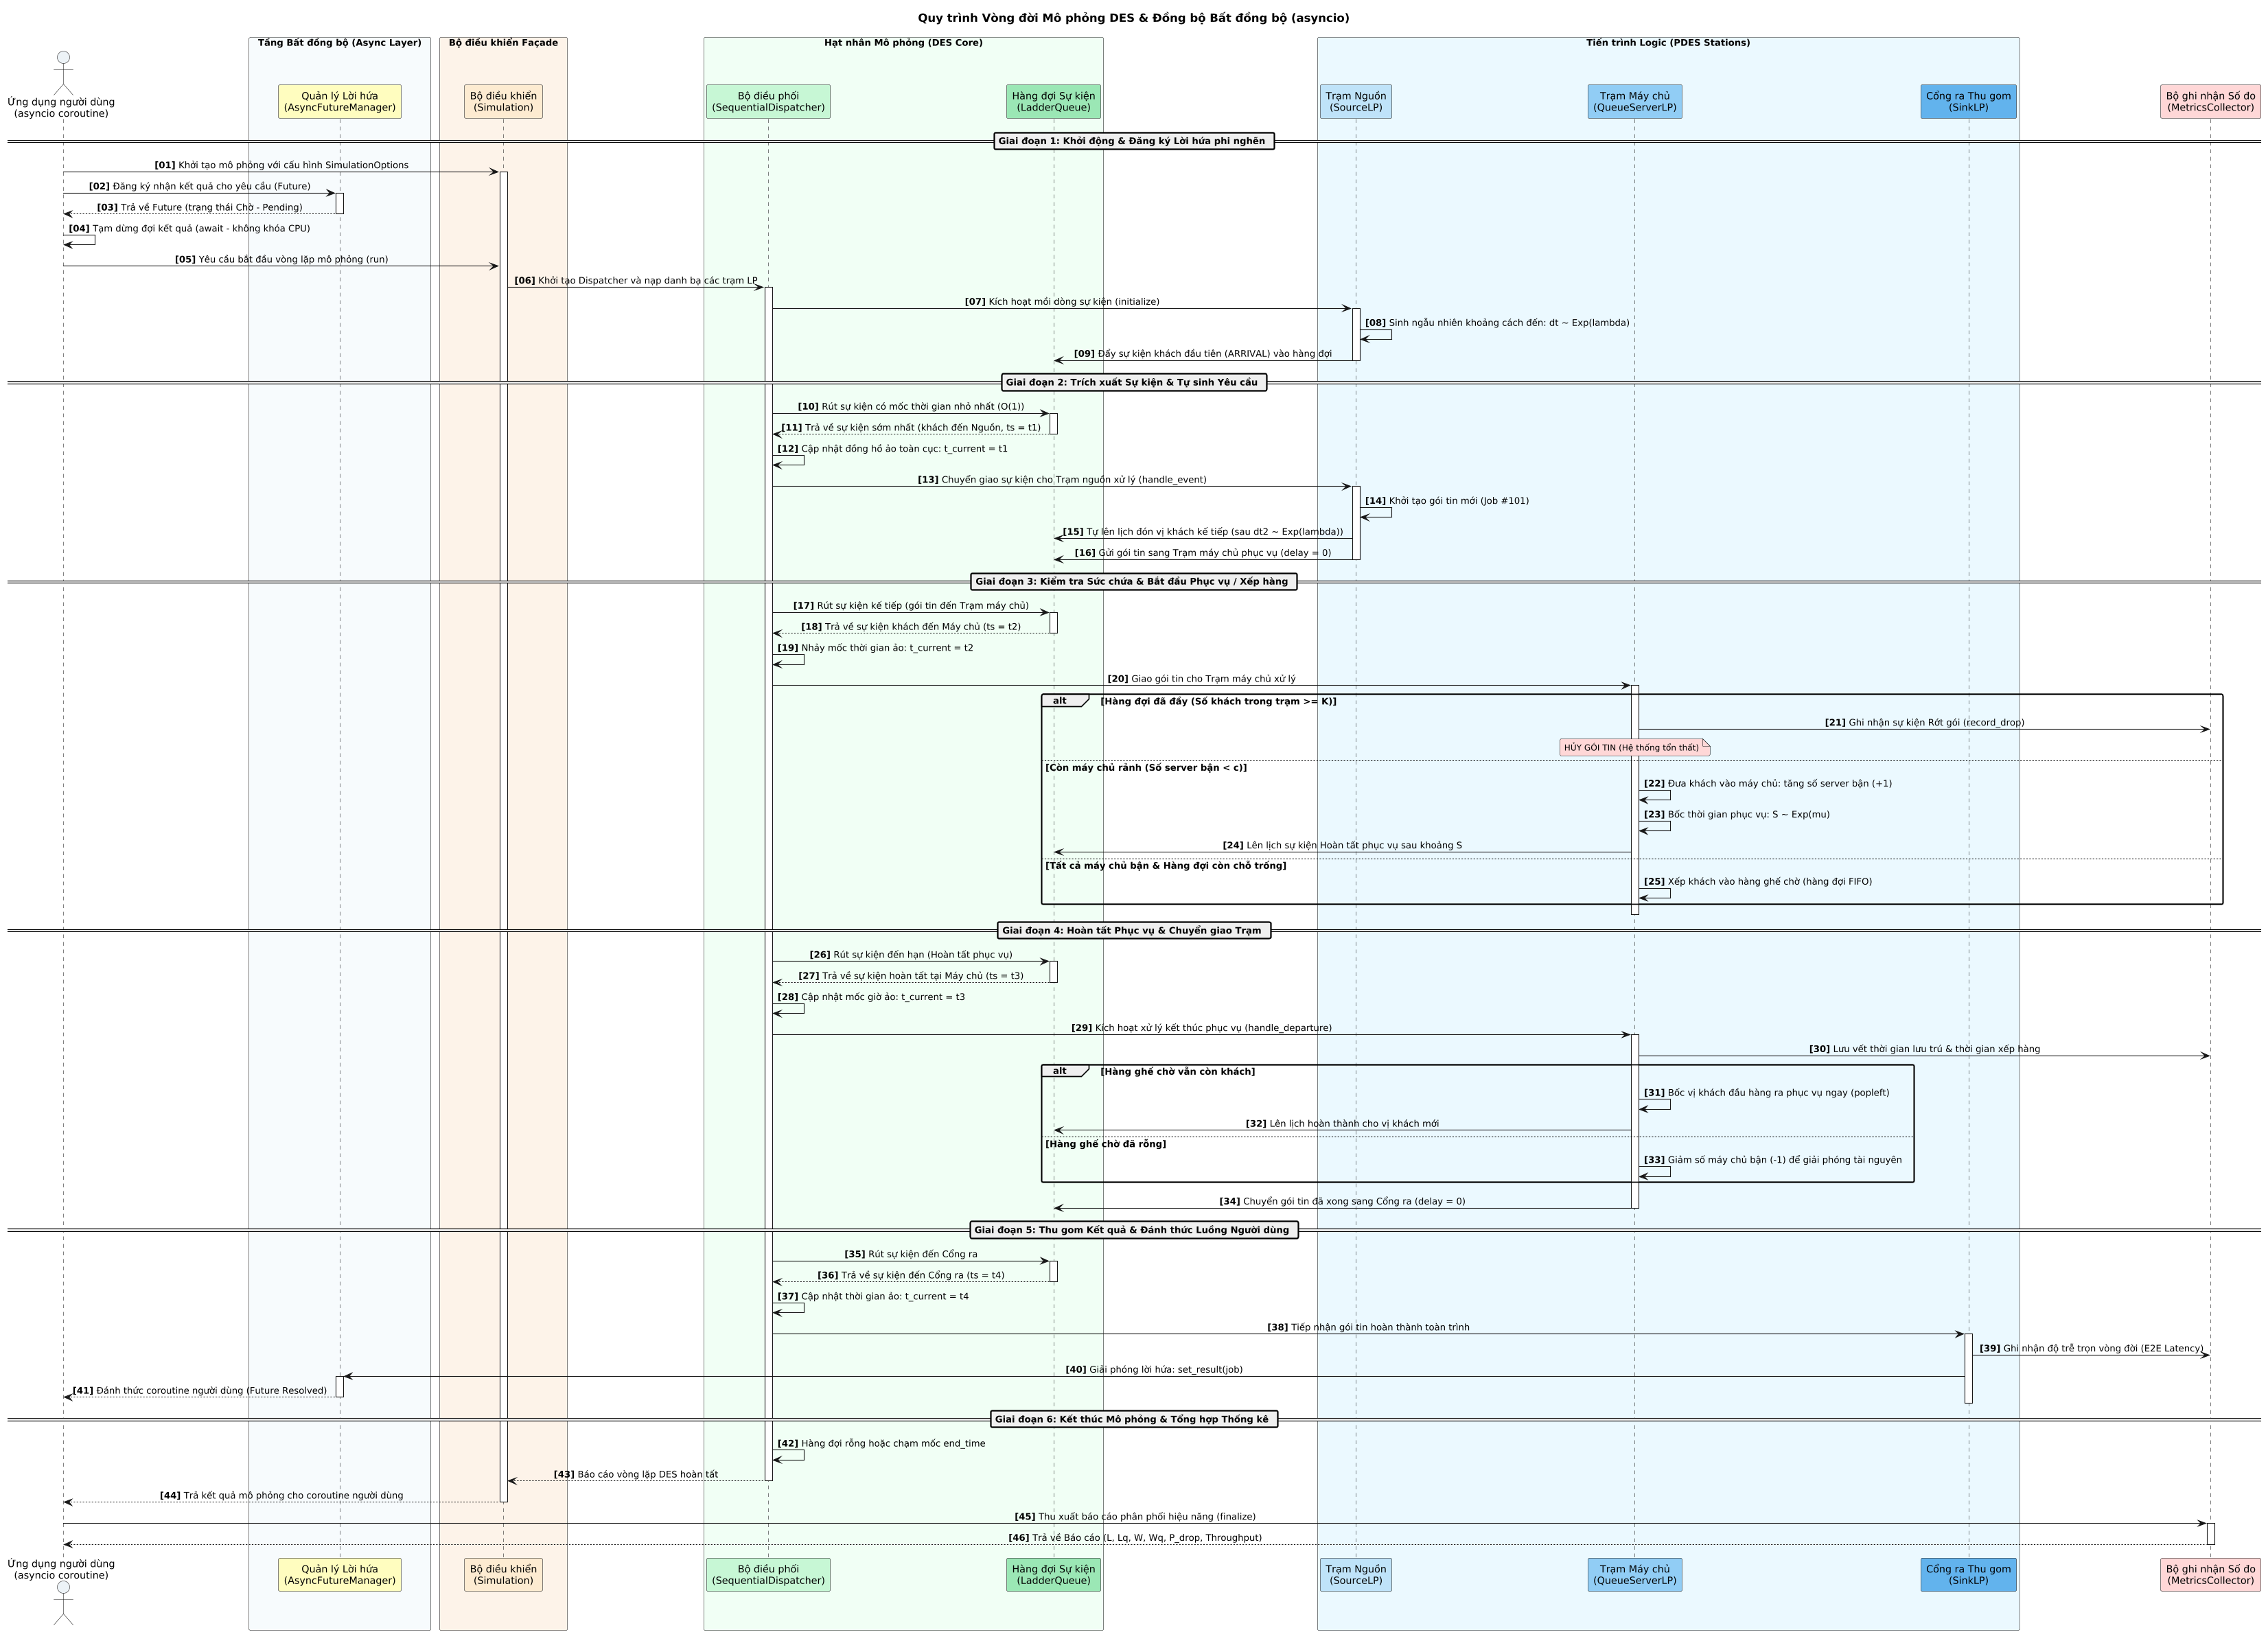
\includegraphics[width=0.95\textwidth]{image/uml_sequence_diagram.png}
\caption{Sơ đồ tuần tự luân chuyển sự kiện (UML Sequence Diagram) trong vòng lặp DES}
\label{fig:uml-sequence-diagram}
\end{figure}

Tiến trình điều phối và xử lý sự kiện trong sơ đồ tuần tự (Hình~\ref{fig:uml-sequence-diagram}) thiết lập cầu nối đồng bộ chặt chẽ giữa tầng ứng dụng bất đồng bộ và hạt nhân mô phỏng rời rạc. Nhằm làm rõ trách nhiệm kiến trúc và giải tỏa sự nhập nhằng giữa các không gian lưu trữ, vai trò cùng cấu trúc dữ liệu nội bộ của từng thực thể tham gia được chú thích chi tiết tại Bảng~\ref{tab:sequence-participants-annotated}.

\begin{table}[H]
\centering
\small
\renewcommand{\arraystretch}{1.25}
\setlength{\tabcolsep}{5pt}
\setlength{\aboverulesep}{0pt}
\setlength{\belowrulesep}{0pt}
\noindent\begin{tabularx}{\linewidth}{>{\small\bfseries\color{bkblue}\raggedright\arraybackslash}p{3.4cm} >{\small\ttfamily\raggedright\arraybackslash}p{3.8cm} >{\small\raggedright\arraybackslash}X}
\arrayrulecolor{bkblue}\toprule[1.5pt]
\rowcolor{bkblue}%
\multicolumn{1}{>{\raggedright\arraybackslash}p{3.4cm}}{\textbf{\color{white}Thành phần}} &
\multicolumn{1}{>{\raggedright\arraybackslash}p{3.8cm}}{\textbf{\color{white}Nơi lưu trữ nội bộ}} &
\multicolumn{1}{>{\raggedright\arraybackslash}X}{\textbf{\color{white}Vai trò \& Hành vi nghiệp vụ tương tác}} \\
\midrule[1pt]
\rowcolor{white}\texttt{User} (Script) & options: \newline SimulationOptions & Điểm khởi tạo cấu hình, nạp mô hình vào Facade và kích hoạt điều phối. \\
\rowcolor{boxbg}\texttt{App} (Coroutine) & -- & Tác vụ coroutine phía người dùng; phát yêu cầu và tạm dừng bằng \texttt{await future} phi phong tỏa luồng. \\
\rowcolor{white}\texttt{Simulation} (Sim) & options, models, \newline lps, dispatcher & Lớp mặt tiền (Facade) quản lý chu trình sống, nạp tự động các LP và kết nối Dispatcher. \\
\rowcolor{boxbg}\texttt{AsyncFutureManager} & \_pending\_futures: \newline Dict[int, Future] & Cầu nối bất đồng bộ; lưu trữ danh bạ lời hứa (\textit{Future}) để đánh thức coroutine khi có kết quả. \\
\rowcolor{white}\texttt{SequentialEvent-}\newline\texttt{Dispatcher} & current\_time, lps, \newline event\_queue, trace\_log & Bộ máy điều phối trung tâm; duy trì mốc $LVT$ toàn cục $t$, trích xuất sự kiện sớm nhất thúc đẩy bước nhảy thời gian. \\
\rowcolor{boxbg}\texttt{LadderQueue} & \_bottom, \_top, \newline \_boundary, bucket\_width & \textbf{Sổ lịch hẹn sự kiện}; hàng đợi ưu tiên phân tầng đạt chi phí $\mathcal{O}(1)$ lưu trữ các bản tin \texttt{Event}. \\
\rowcolor{white}\texttt{SourceLP} & local\_virt\_time, \newline \_started, \_job\_counter & Cổng phát sinh tải Poisson; khi mồi sự kiện sẽ tự động lên lịch đón vị khách kế tiếp sau $\Delta t \sim \text{Exp}(\lambda)$. \\
\rowcolor{boxbg}\texttt{QueueServerLP} & waiting\_queue (FIFO), \newline busy\_servers, metrics & Trạm máy chủ kèm bộ đệm; quản lý \textbf{hàng ghế chờ FIFO} lưu \texttt{Job} khi cả $c$ máy chủ đều bận. \\
\rowcolor{white}\texttt{SinkLP} & completed\_jobs, \newline total\_response\_times & Cổng ra thu gom; điểm kết thúc hành trình của \texttt{Job}, tính trễ toàn trình $W$ và kích hoạt giải phóng \texttt{Future}. \\
\rowcolor{boxbg}\texttt{MetricsCollector} & waiting\_times, \newline \_area\_q\_len, \_area\_in\_sys & Bộ tích lũy số đo; tính tích phân thời gian $\sum \text{State} \cdot \Delta t$ để xác định $W, W_q, L, L_q, \rho, P_b$. \\
\arrayrulecolor{bkblue}\bottomrule[1.5pt]
\end{tabularx}
\caption{Bảng chú thích vai trò và cấu trúc lưu trữ của các thực thể tham gia sơ đồ tuần tự}
\label{tab:sequence-participants-annotated}
\end{table}

Dựa trên sự phân công trách nhiệm rành mạch trên, toàn bộ tiến trình điều phối và luân chuyển sự kiện được phân tầng thành 6 giai đoạn kỹ thuật rõ rệt, gắn kết trực tiếp với các bước tương tác từ \textbf{[01]} đến \textbf{[46]}:

\begin{enumerate}[leftmargin=2em, itemsep=6pt]
\item \textbf{Giai đoạn 1: Khởi động \& Đăng ký Lời hứa phi nghẽn (Bước [01] -- [09]):}
\begin{itemize}[leftmargin=1.5em, itemsep=2pt]
\item \textit{Đăng ký Promise:} Coroutine phía người dùng gọi phương thức \texttt{register\_promise()} tới \texttt{AsyncFutureManager}. Trình quản lý khởi tạo đối tượng \texttt{asyncio.Future}, lưu trữ vào bảng tra cứu \texttt{\_pending\_futures} và trao lại đối tượng này cho người dùng. Ứng dụng thực hiện \texttt{await future} để tạm dừng luồng gọi mà hoàn toàn không phong tỏa luồng điều phối chính.
\item \textit{Mồi luồng sự kiện:} Hệ thống kích hoạt phương thức \texttt{start()} tại trạm \texttt{SourceLP}. Trạm nguồn bốc mẫu ngẫu nhiên khoảng thời gian đến đầu tiên $\Delta t_1 \sim \text{Exp}(\lambda)$, đóng gói thành bản tin \texttt{Event(type=ARRIVAL, dest='Source', timestamp=$\Delta t_1$)} và đẩy trực tiếp vào hàng đợi ưu tiên \texttt{EventQueue}.
\end{itemize}

\item \textbf{Giai đoạn 2: Trích xuất Sự kiện \& Tự sinh Yêu cầu (Bước [10] -- [16]):}
\begin{itemize}[leftmargin=1.5em, itemsep=2pt]
\item \textit{Bước nhảy thời gian ảo:} \texttt{Dispatcher} thực hiện thao tác \texttt{queue.pop()} lấy sự kiện có nhãn thời gian sớm nhất ra khỏi \texttt{EventQueue} và cập nhật trục thời gian ảo toàn cục: $t_{\text{current}} = t_1$. Mọi khoảng thời gian trống từ $0.00$ đến $t_1$ được bỏ qua tức thời.
\item \textit{Tự sinh dòng Poisson vô hạn:} Sự kiện được chuyển giao cho \texttt{SourceLP} để khởi tạo một thực thể \texttt{Job} mới (chứa mã định danh \texttt{job\_id} và mốc giờ đến \texttt{arrival\_time} = $t_1$). Đồng thời, trạm tự lên lịch cho chính mình sự kiện khách đến kế tiếp sau độ trễ $\Delta t_2 \sim \text{Exp}(\lambda)$ và ném vào \texttt{EventQueue} nhằm duy trì dòng khách liên tục. Ngay sau đó, trạm chuyển tiếp gói tin sang \texttt{QueueServerLP} với độ trễ chuyển mạch bằng 0 (tức thời tại mốc $t_1$).
\end{itemize}

\item \textbf{Giai đoạn 3: Phân phối \& Kiểm tra Sức chứa tại Máy chủ (Bước [17] -- [25]):}
\begin{itemize}[leftmargin=1.5em, itemsep=2pt]
\item \texttt{Dispatcher} tiếp tục lấy sự kiện đến chuyển cho \texttt{QueueServerLP.handle\_event(e)}.
\item \textit{Cơ chế kiểm soát đệm $K$:} Máy chủ kiểm tra ngưỡng dung lượng trạm: nếu số khách hiện hữu trong trạm (bao gồm số khách đang được phục vụ cộng với số khách đang ngồi chờ) đã đạt trần $K$ ($N(t) = \text{busy} + \text{len(waiting\_queue)} \ge K$), gói tin bị hủy bỏ ngay lập tức (\textit{Packet Dropped}) và cập nhật tổn thất vào \texttt{MetricsCollector}.
\item \textit{Phân bổ phục vụ hoặc xếp hàng chờ:} Nếu trạm còn chỗ:
\begin{itemize}[leftmargin=1.2em, itemsep=1pt]
\item Khi có ít nhất một máy chủ rảnh rỗi ($\text{busy\_servers} < c$): Yêu cầu \texttt{Job} được đưa thẳng vào phục vụ ngay (thời gian chờ $W_q = 0$). Trạm tăng bộ đếm $\text{busy\_servers} \leftarrow \text{busy\_servers} + 1$, bốc ngẫu nhiên thời gian phục vụ $S \sim \text{Exp}(\mu)$ và tạo sự kiện hoàn tất trong tương lai \texttt{Event(type=DEPARTURE, timestamp=$t + S$)} đẩy vào \texttt{EventQueue}.
\item Khi tất cả $c$ máy chủ đều đang bận ($\text{busy\_servers} = c$): Yêu cầu \texttt{Job} được đưa vào \textbf{hàng ghế chờ FIFO} \texttt{waiting\_queue.append(job)} nằm bên trong trạm để kiên nhẫn đợi đến lượt.
\end{itemize}
\end{itemize}

\item \textbf{Giai đoạn 4: Hoàn tất Phục vụ \& Chuyển giao Trạm (Bước [26] -- [34]):}
\begin{itemize}[leftmargin=1.5em, itemsep=2pt]
\item Khi trục thời gian ảo tiến tới mốc hoàn thành $t_{\text{current}} = t + S$, \texttt{Dispatcher} kích hoạt sự kiện \texttt{DEPARTURE} tại \texttt{QueueServerLP}.
\item Máy chủ ghi nhận thời gian lưu trú và thời gian chờ vào \texttt{MetricsCollector}. Sau đó kiểm tra hàng ghế chờ:
\begin{itemize}[leftmargin=1.2em, itemsep=1pt]
\item Nếu \texttt{waiting\_queue} còn khách: Trạm lập tức bốc vị khách đầu hàng ra xử lý (\texttt{waiting\_queue.popleft()}), bốc thời gian phục vụ mới $S'$ và lên lịch sự kiện \texttt{DEPARTURE} tiếp theo vào \texttt{EventQueue}.
\item Nếu \texttt{waiting\_queue} rỗng: Trạm giảm bộ đếm máy chủ bận ($\text{busy\_servers} \leftarrow \max(0, \text{busy} - 1)$) để hoàn trả tài nguyên máy chủ về trạng thái rảnh rỗi.
\end{itemize}
\item Gói tin đã xử lý xong được chuyển tiếp sang cổng ra \texttt{SinkLP} với độ trễ bằng 0.
\end{itemize}

\item \textbf{Giai đoạn 5: Thu gom Kết quả \& Giải phóng Lời hứa (Bước [35] -- [41]):}
\begin{itemize}[leftmargin=1.5em, itemsep=2pt]
\item \texttt{SinkLP} tiếp nhận gói tin hoàn tất, tính toán độ trễ toàn trình $T = t_{\text{dep}} - t_{\text{arr}}$ và ghi nhận vào \texttt{MetricsCollector}.
\item Trạm gọi phương thức \texttt{set\_result(job\_id, job)} trên \texttt{AsyncFutureManager}. Trình quản lý tra cứu mã yêu cầu trong bảng \texttt{\_pending\_futures}, gán giá trị kết quả và giải phóng \texttt{Future}. Lập tức coroutine phía người dùng đang dừng ở lệnh \texttt{await} được đánh thức để nhận kết quả trong thời gian thực mà không làm phong tỏa tiến trình mô phỏng rời rạc.
\end{itemize}

\item \textbf{Giai đoạn 6: Kết thúc Mô phỏng \& Tổng hợp Thống kê (Bước [42] -- [46]):}
\begin{itemize}[leftmargin=1.5em, itemsep=2pt]
\item Khi chạm mốc thời gian kết thúc $T_{\text{end}}$ hoặc \texttt{EventQueue} cạn kiệt phần tử, \texttt{Dispatcher} dừng vòng lặp điều phối và phát thông báo hoàn tất tới ứng dụng.
\item Ứng dụng người dùng kích hoạt phương thức trích xuất báo cáo từ \texttt{MetricsCollector} để thu được toàn bộ vector chỉ số hiệu năng chuẩn xác ($W, W_q, L, L_q, P_b, \lambda_{\text{eff}}$).
\end{itemize}
\end{enumerate}

\begin{table}[H]
\centering
\small
\renewcommand{\arraystretch}{1.35}
\setlength{\tabcolsep}{5pt}
\setlength{\aboverulesep}{0pt}
\setlength{\belowrulesep}{0pt}
\noindent\begin{tabularx}{\linewidth}{>{\ttfamily\bfseries\color{bkblue}\raggedright\arraybackslash}p{2.2cm} >{\ttfamily\raggedright\arraybackslash}p{3.2cm} >{\ttfamily\raggedright\arraybackslash}p{2.6cm} >{\centering\arraybackslash}p{1.6cm} >{\raggedright\arraybackslash}X}
\arrayrulecolor{bkblue}\toprule[1.5pt]
\rowcolor{bkblue}%
\multicolumn{1}{>{\raggedright\arraybackslash}p{2.2cm}}{\textbf{\color{white}Kiểu sự kiện}} &
\multicolumn{1}{>{\raggedright\arraybackslash}p{3.2cm}}{\textbf{\color{white}Thực thể phát}} &
\multicolumn{1}{>{\raggedright\arraybackslash}p{2.6cm}}{\textbf{\color{white}Thực thể nhận}} &
\multicolumn{1}{>{\centering\arraybackslash}p{1.6cm}}{\textbf{\color{white}Độ trễ $\Delta t$}} &
\multicolumn{1}{>{\raggedright\arraybackslash}X}{\textbf{\color{white}Hành vi nghiệp vụ kích hoạt}} \\
\midrule[1pt]
\rowcolor{white}ARRIVAL & SourceLP & SourceLP & $\text{Exp}(\lambda)$ & Tự sinh khách kế tiếp và duy trì dòng Poisson \\
\rowcolor{boxbg}ARRIVAL & SourceLP & QueueServerLP & $0.0$ & Chuyển Job mới đến kiểm tra dung lượng bộ đệm $K$ \\
\rowcolor{white}DEPARTURE & QueueServerLP & QueueServerLP & $\text{Exp}(\mu)$ & Hoàn tất phục vụ, giải phóng server, đón khách chờ \\
\rowcolor{boxbg}ARRIVAL & BranchingServerLP & Printer / Disk & $0.0$ & Rẽ nhánh xác suất ($p=0.3$ Máy in, $p=0.7$ Ổ đĩa) \\
\rowcolor{white}ARRIVAL & Server / Disk & SinkLP & $0.0$ & Ghi nhận trễ toàn trình và kích hoạt \texttt{set\_result()} \\
\rowcolor{boxbg}TERMINATE & Dispatcher & Dispatcher & $T_{\text{end}}$ & Dừng vòng lặp điều phối và tổng kết kết quả \\
\arrayrulecolor{bkblue}\bottomrule[1.5pt]
\end{tabularx}
\caption{Ma trận thông điệp sự kiện luân chuyển giữa các thành phần}
\label{tab:sequence-matrix}
\end{table}

% Ma trận trên khẳng định hai đặc tính then chốt trong cơ chế luân chuyển sự kiện:
% \begin{itemize}[leftmargin=1.5em, itemsep=2pt]
% \item \textbf{Phân ly lỏng (Loose Coupling):} Các trạm logic hoàn toàn không gọi trực tiếp phương thức của nhau mà chỉ tương tác gián tiếp thông qua việc phát sinh bản tin \texttt{Event} đẩy vào hàng đợi trung tâm.
% \item \textbf{Đồng bộ bước nhảy thời gian:} Ngoại trừ các sự kiện có độ trễ ngẫu nhiên (sinh khách $\text{Exp}(\lambda)$ và phục vụ $\text{Exp}(\mu)$), mọi sự kiện chuyển tiếp nội bộ giữa các trạm đều được xử lý với độ trễ chuyển mạch bằng 0 (tức thời tại cùng mốc thời gian ảo).
% \end{itemize}


% \textbf{Kịch bản số học minh họa trực quan tiến trình luân chuyển sự kiện (Trace Walkthrough):}

% Để làm sáng tỏ tính tương tác giữa các thành phần trong không gian thời gian ảo, kịch bản dưới đây minh họa vết thực thi số học cụ thể trên cấu hình hàng đợi đơn máy chủ $M/M/1/5$ ($c=1, K=5$) qua Bảng~\ref{tab:numerical-trace-walkthrough}:

% \begin{table}[H]
% \centering
% \small
% \renewcommand{\arraystretch}{1.3}
% \setlength{\tabcolsep}{5pt}
% \setlength{\aboverulesep}{0pt}
% \setlength{\belowrulesep}{0pt}
% \noindent\begin{tabularx}{\linewidth}{>{\centering\arraybackslash\bfseries\color{bkblue}}p{1.7cm} >{\ttfamily\raggedright\arraybackslash}p{2.3cm} >{\ttfamily\raggedright\arraybackslash}p{2.5cm} >{\centering\arraybackslash}p{2.8cm} >{\raggedright\arraybackslash}X}
% \arrayrulecolor{bkblue}\toprule[1.5pt]
% \rowcolor{bkblue}%
% \multicolumn{1}{>{\centering\arraybackslash}p{1.8cm}}{\textbf{\color{white}Mốc giờ $t$}} &
% \multicolumn{1}{>{\raggedright\arraybackslash}p{2.3cm}}{\textbf{\color{white}Sự kiện kích hoạt}} &
% \multicolumn{1}{>{\raggedright\arraybackslash}p{2.5cm}}{\textbf{\color{white}Trạm xử lý}} &
% \multicolumn{1}{>{\centering\arraybackslash}p{2.8cm}}{\textbf{\color{white}Trạng thái trạm}} &
% \multicolumn{1}{>{\raggedright\arraybackslash}X}{\textbf{\color{white}Hành vi nghiệp vụ \& Biến động số đo}} \\
% \midrule[1pt]
% \rowcolor{white}$t = 0.00$ & Khởi động & SourceLP & $\text{busy}=0, Q=0$ & Mồi hệ thống: sinh $\Delta t_1 = 1.20$, đẩy $e_1(\text{ARRIVAL}, t=1.20)$ vào \texttt{EventQueue}. \\
% \rowcolor{boxbg}$t = 1.20$ & ARRIVAL (Source) & SourceLP & $\text{busy}=0, Q=0$ & Khởi tạo yêu cầu $J_1$, tự hẹn khách $J_2$ tại $t=2.80$, chuyển $J_1$ sang trạm máy chủ. \\
% \rowcolor{white}$t = 1.20$ & ARRIVAL (Server) & QueueServerLP & $\text{busy}=1, Q=0$ & Máy chủ rảnh $\to$ phục vụ $J_1$ ngay ($W_{q,1} = 0.00$). Bốc $S_1 = 1.50$, hẹn xong tại $t=2.70$. \\
% \rowcolor{boxbg}$t = 2.70$ & DEPARTURE & QueueServerLP & $\text{busy}=0, Q=0$ & Hoàn tất $J_1$, giải phóng máy chủ (hàng chờ rỗng), chuyển $J_1$ sang cổng ra \texttt{SinkLP}. \\
% \rowcolor{white}$t = 2.70$ & ARRIVAL (Sink) & SinkLP & $\text{busy}=0, Q=0$ & Ghi nhận độ trễ $T_1 = 1.50$s. Gọi \texttt{set\_result()} $\to$ Đánh thức coroutine \texttt{await}. \\
% \rowcolor{boxbg}$t = 2.80$ & ARRIVAL (Server) & QueueServerLP & $\text{busy}=1, Q=0$ & Khách $J_2$ đến; do máy chủ đã giải phóng tại $t=2.70$, $J_2$ được phục vụ ngay lập tức. \\
% \arrayrulecolor{bkblue}\bottomrule[1.5pt]
% \end{tabularx}
% \caption{Bảng diễn biến vết thực thi sự kiện số học (Numerical Trace Walkthrough)}
% \label{tab:numerical-trace-walkthrough}
% \end{table}

% Qua bảng diễn biến trên, hai đặc tính then chốt của kiến trúc DES được kiểm chứng rõ nét:
% \begin{itemize}[leftmargin=1.5em, itemsep=2pt]
% \item \textbf{Tính phi nghẽn tuyệt đối:} Mọi tính toán diễn ra tức thời tại các mốc biến cố rời rạc ($0.00 \to 1.20 \to 2.70 \to 2.80$). Trục thời gian máy tính không hề bị lãng phí cho các khoảng thời gian hệ thống nhàn rỗi ($t \in (0.00, 1.20)$ hay $t \in (2.70, 2.80)$).
% \item \textbf{Tính bảo toàn nhân quả:} Không xuất hiện bất kỳ sự kiện nào có mốc thời gian ngược về quá khứ; trật tự các bước tuân thủ nghiệm ngặt thứ tự ưu tiên của hàng đợi Min-Heap.
% \end{itemize}
\newpage
% =========================================================================
\subsection{Kiến trúc điều phối cốt lõi của bộ mô phỏng DES (Core DES Dispatching Architecture)}
\label{subsec:core-des-engine}
% =========================================================================
\subsubsection{Cấu trúc Lớp Bản ghi Sự kiện (\texttt{Event}) và Cơ chế So sánh theo Thời gian ảo (Timestamp Ordering)}
\label{subsubsec:event-structure}

\hspace{0.5cm}Trong mô phỏng DES, toàn bộ động thái của hệ thống được kích hoạt bằng các bản tin sự kiện (\texttt{Event}). Để tối ưu hóa hiệu năng trích xuất và bảo đảm tính tiền định (\textit{Determinism}), hệ thống áp dụng cơ chế so sánh tự nhiên dựa trên mốc thời gian ảo \texttt{timestamp}:

\begin{equation}
e_1 < e_2 \iff e_1.\text{timestamp} < e_2.\text{timestamp}
\end{equation}
trong đó:
\begin{itemize}[leftmargin=2em, itemsep=1pt]
\item $e.\text{timestamp}$: Mốc thời gian ảo mà sự kiện sẽ nổ ra (tiêu chí so sánh tự nhiên duy nhất theo khai báo \texttt{@dataclass(order=True)}).
\item $e.\text{sender\_id}$: Mã định danh tiến trình logic phát sinh sự kiện (hỗ trợ alias property \texttt{source\_lp}).
\item $e.\text{receiver\_id}$: Mã định danh tiến trình logic tiếp nhận sự kiện (hỗ trợ alias property \texttt{dest\_lp}).
\item $e.\text{event\_type}$: Kiểu sự kiện trong mô hình rời rạc (\texttt{ARRIVAL}, \texttt{SERVICE\_START}, \texttt{DEPARTURE},...).
\item $e.\text{payload}$: Tải trọng dữ liệu đi kèm gói tin (chứa đối tượng \texttt{Job} hoặc từ điển dữ liệu, hỗ trợ alias property \texttt{data}).
\item $e.\text{event\_id}$: Chuỗi định danh duy nhất của sự kiện dạng UUID4 tự sinh.
\end{itemize}

\begin{lstlisting}[language=Python, caption={Cấu trúc sự kiện Event và cơ chế so sánh theo thời gian ảo (bkitevsim/core/event.py)}, label={lst:event-core}]
from __future__ import annotations
from dataclasses import dataclass, field
from enum import Enum, auto
import uuid
from typing import Any, Optional

class EventType(Enum):
    """Event types supported in discrete-event queuing models."""
    ARRIVAL = auto()        # Customer or packet arrives at a station
    SERVICE_START = auto()  # Server starts servicing a waiting customer
    DEPARTURE = auto()      # Service complete; packet departs station
    IO_COMPLETE = auto()    # I/O peripheral data transfer completed
    MESSAGE = auto()        # Inter-LP asynchronous coordination message
    TERMINATE = auto()      # Triggers simulation engine termination

@dataclass(order=True)
class Event:
    """Represents a discrete event in the simulation (PDES model).

    Events are ordered by timestamp for priority queue operations.
    The order=True parameter generates natural comparison based on timestamp.
    """
    # --- 1st key: Earliest virtual time (LVT) ---
    timestamp: float
    # --- Domain attributes (excluded from heap comparisons via compare=False) 
    sender_id: Any = field(compare=False, default=0)
    receiver_id: Any = field(compare=False, default=0)
    event_type: Any = field(compare=False, default="EVENT")
    payload: Any = field(compare=False, default=None)
    event_id: Any = field(compare=False, default_factory=lambda: str(uuid.uuid4()))

    def __init__(
        self,
        timestamp: float = 0.0,
        sender_id: Any = None,
        receiver_id: Any = None,
        event_type: Any = "EVENT",
        payload: Any = None,
        event_id: Any = None,
        **kwargs: Any
    ) -> None:
        self.timestamp = float(timestamp)
        # Handle source / sender aliases
        self.sender_id = sender_id if sender_id is not None else kwargs.get("source_lp", 0)
        # Handle destination / receiver aliases
        self.receiver_id = receiver_id if receiver_id is not None else kwargs.get("dest_lp", 0)
        self.event_type = event_type.name if hasattr(event_type, "name") else str(event_type)
        self.payload = payload if payload is not None else kwargs.get("data", None)
        self.event_id = str(event_id) if event_id is not None else str(uuid.uuid4())
        self._priority = kwargs.get("priority", 0)

        # Validation: Enforce non-negative timestamps
        if self.timestamp < 0:
            raise ValueError(f"Event timestamp cannot be negative: {self.timestamp}")

    @property
    def source_lp(self) -> Any:
        return self.sender_id

    @property
    def dest_lp(self) -> Any:
        return self.receiver_id
\end{lstlisting}

\newpage
\textbf{Phân tích kỹ thuật chuyên sâu về Phòng vệ kiểu dữ liệu và Cơ chế so sánh trong \texttt{bkitevsim}:}

Để hiểu rõ tại sao kiến trúc lớp \texttt{Event} trong gói \texttt{bkitevsim} mang tính quyết định đến độ ổn định của toàn bộ hệ thống mô phỏng, cần phân tích nguy cơ kỹ thuật tiềm ẩn trong các hệ thống DES hướng đối tượng:
\begin{itemize}[leftmargin=1.5em, itemsep=3pt]
\item \textbf{Cơ chế định thời tự nhiên qua \texttt{@dataclass(order=True)}:} Tiêu chí cốt lõi của DES là nguyên lý nhân quả: sự kiện có mốc thời gian ảo nhỏ hơn bắt buộc phải được trích xuất và kích hoạt trước. Bằng cách khai báo \texttt{timestamp: float} là trường so sánh duy nhất và kích hoạt \texttt{order=True}, Python tự động sinh các phương thức so sánh quan hệ (\texttt{\_\_lt\_\_}, \texttt{\_\_gt\_\_},...) thuần túy dựa trên biến số thực \texttt{timestamp}, giúp các cấu trúc hàng đợi ưu tiên (\texttt{MinHeapPriorityQueue} và \texttt{LadderQueue}) đạt tốc độ so sánh cực đại $\mathcal{O}(1)$ trên thanh ghi CPU.
\item \textbf{Phòng vệ ngoại lệ thời gian chạy (\textit{Runtime Exception Prevention}):} Nhờ thiết lập \texttt{compare=False}, trong ngôn ngữ Python, nếu hai đối tượng dataclass có trường so sánh đầu tiên bằng nhau ($e_1.\text{timestamp} == e_2.\text{timestamp}$), module \texttt{heapq} sẽ tự động so sánh trường tiếp theo được định nghĩa trong lớp. Nếu không thiết lập tường minh, bộ so sánh sẽ chạm vào trường \texttt{payload} chứa kiểu dữ liệu từ điển (\texttt{dict}) hoặc đối tượng nghiệp vụ phức tạp. Do Python không hỗ trợ toán tử so sánh $<$ giữa hai từ điển, chương trình sẽ lập tức ném ngoại lệ:
\begin{center}
\texttt{TypeError: '<' not supported between instances of 'dict'}
\end{center}
làm sập toàn bộ tiến trình mô phỏng ngay tại thời gian chạy. Trong gói \texttt{bkitevsim}, việc cấu hình tường minh \texttt{compare=False} cho toàn bộ các trường còn lại (\texttt{sender\_id}, \texttt{receiver\_id}, \texttt{event\_type}, \texttt{payload}, \texttt{event\_id}) là giải pháp phòng vệ kiến trúc mang tính sống còn, cô lập hoàn toàn phép so sánh heap chỉ vào biến số thực \texttt{timestamp}.
\item \textbf{Hệ thống thuộc tính tương thích ngược (\textit{Backward Compatibility Properties}):} Nhằm dung hòa giữa chuẩn thiết kế mới của gói \texttt{bkitevsim} (sử dụng danh pháp chuẩn PDES \texttt{sender\_id}, \texttt{receiver\_id}, \texttt{payload}) và các kịch bản mô phỏng kiểm thử cũ, lớp \texttt{Event} cung cấp sẵn hệ thống getter property (\texttt{source\_lp}, \texttt{dest\_lp}, \texttt{data}, \texttt{priority}), cho phép mã nguồn ngoài truy cập nhất quán mà không làm thay đổi cấu trúc lưu trữ nội bộ.
\end{itemize}

\newpage
\subsubsection{Cấu trúc hàng đợi sự kiện phân tầng hai cấp (LadderQueue)}
\label{subsubsec:ladder-queue}

\hspace{0.5cm}Cấu trúc Min-Heap nhị phân chuẩn sở hữu chi phí chèn và xóa là $O(\log N)$. Khi số lượng sự kiện mô phỏng vượt ngưỡng $10^6$, độ sâu của cây Heap làm suy giảm nghiêm trọng băng thông xử lý của CPU.

Để giải quyết vấn đề này, nhóm đã hiện thực thuật toán \textbf{\texttt{LadderQueue}} phân tầng hai cấp (Hình~\ref{fig:ladder-queue-arch}):
\begin{itemize}[leftmargin=1.5em, itemsep=3pt]
\item \textbf{Tầng dưới (\texttt{\_bottom}):} Lưu trữ tập hợp các sự kiện sắp xảy ra trong một cửa sổ thời gian gần $[t_{\text{current}}, \text{\_boundary}]$. Do số lượng phần tử nhỏ, thao tác trích xuất đạt hiệu năng tối ưu $O(1)$.
\item \textbf{Tầng trên (\texttt{\_top}):} Lưu trữ các sự kiện thuộc tương lai xa ($t > \text{\_boundary}$).
\item \textbf{Bất biến phân tầng (\textit{Tiered Invariant}):} Duy trì đẳng thức:
\begin{equation}
\max_{e \in \text{\_bottom}} (e.\text{timestamp}) \le \text{\_boundary} < \min_{e \in \text{\_top}} (e.\text{timestamp})
\end{equation}
\item \textbf{Cơ chế nạp tầng (\textit{Rung Refill}):} Khi tầng \texttt{\_bottom} cạn kiệt, thuật toán xác định ranh giới mới $\text{\_boundary} = \min(\text{\_top}) + \text{rung\_width}$ và trút các sự kiện thỏa điều kiện từ tầng trên xuống tầng dưới.
\end{itemize}

\begin{figure}[H]
\centering
\begin{tikzpicture}[scale=0.92, every node/.style={transform shape}]
% ==============================================================
% 1. TẦNG TRÊN (TOP HEAP) - LƯU SỰ KIỆN TƯƠNG LAI
% ==============================================================
% Khung bao ngoai Top Heap (shifted by +0.9)
\draw[thick, fill=gray!6, draw=gray!60, rounded corners=6pt] (0, 6.2) rectangle (14.6, 8.7);

% Header banner Top Heap
\path[fill=gray!22, rounded corners=6pt] (0, 8.0) rectangle (14.6, 8.7);
\path[fill=gray!22] (0, 8.0) rectangle (14.6, 8.2);
\draw[draw=gray!50, thick] (0, 8.0) -- (14.6, 8.0);

\node[anchor=west, font=\bfseries\footnotesize\color{black!80}] at (0.35, 8.35) 
{TẦNG ĐỈNH: Top Heap ($t > \text{boundary}$)};
\node[anchor=east, font=\scriptsize\bfseries, fill=gray!75!black, text=white, rounded corners=3pt, inner sep=3.5pt] at (14.25, 8.35) 
{Min-Heap: $\mathcal{O}(\log N)$};

% Cac the su kien trong Top Heap
\draw[fill=white, draw=gray!70, rounded corners=3pt, line width=0.8pt] (0.6, 6.7) rectangle (2.2, 7.7);
\node[font=\footnotesize\bfseries\color{black!85}] at (1.4, 7.35) {$e_5$};
\node[font=\scriptsize\color{black!70}] at (1.4, 6.95) {$t = 5.6$};

\draw[fill=white, draw=gray!70, rounded corners=3pt, line width=0.8pt] (2.5, 6.7) rectangle (4.1, 7.7);
\node[font=\footnotesize\bfseries\color{black!85}] at (3.3, 7.35) {$e_6$};
\node[font=\scriptsize\color{black!70}] at (3.3, 6.95) {$t = 7.2$};

\draw[fill=white, draw=gray!70, rounded corners=3pt, line width=0.8pt] (4.4, 6.7) rectangle (6.0, 7.7);
\node[font=\footnotesize\bfseries\color{black!85}] at (5.2, 7.35) {$e_7$};
\node[font=\scriptsize\color{black!70}] at (5.2, 6.95) {$t = 8.9$};

\draw[fill=white, draw=gray!70, rounded corners=3pt, line width=0.8pt] (6.3, 6.7) rectangle (7.9, 7.7);
\node[font=\footnotesize\bfseries\color{black!85}] at (7.1, 7.35) {$e_8$};
\node[font=\scriptsize\color{black!70}] at (7.1, 6.95) {$t = 12.4$};

\node[font=\Large\bfseries\color{gray!80}] at (8.6, 7.2) {$\cdots$};

\draw[fill=white, draw=gray!70, rounded corners=3pt, line width=0.8pt] (9.3, 6.7) rectangle (11.1, 7.7);
\node[font=\footnotesize\bfseries\color{black!85}] at (10.2, 7.35) {$e_N$};
\node[font=\scriptsize\color{black!70}] at (10.2, 6.95) {$t = 4980.2$};

% The chu thich dac tinh Top Heap ben phai
\draw[fill=gray!15, draw=gray!40, rounded corners=3pt] (11.5, 6.7) rectangle (14.1, 7.7);
\node[font=\scriptsize\bfseries\color{black!75}] at (12.8, 7.35) {Cấu trúc Min-Heap};
\node[font=\tiny\color{black!60}] at (12.8, 6.95) {Độ sâu cây: $\sim \log_2 N$};

\node[anchor=west, font=\scriptsize\itshape\color{black!60}] at (0.6, 6.42) 
{* Lưu trữ $N$ sự kiện phát sinh xa trong tương lai; giảm thiểu tần suất tái sắp xếp cho CPU};

% ==============================================================
% 2. VÙNG CHUYỂN TIẾP: CƠ CHẾ NẠP TẦNG (RUNG REFILL)
% ==============================================================
% Hop thong tin Rung Refill o giua (shifted by +0.5)
\draw[fill=orange!7, draw=orange!75!black, line width=1pt, rounded corners=5pt] (1.5, 4.3) rectangle (13.1, 5.5);
\node[font=\bfseries\scriptsize\color{orange!95!black}] at (7.3, 5.15) 
{CƠ CHẾ NẠP TẦNG (RUNG REFILL) --- Kích hoạt khi Tầng Đáy rỗng};
\node[font=\scriptsize\color{black!85}] at (7.3, 4.80) 
{1. Thiết lập mốc mới: $\text{\_boundary} \leftarrow \min(e.\text{timestamp} \in \text{\_top}) + \text{rung\_width}$};
\node[font=\scriptsize\color{black!85}] at (7.3, 4.48) 
{2. Di chuyển các sự kiện thỏa $t \in [\min(\text{top}), \text{\_boundary}]$ nạp xuống Tầng Đáy};

% Mui ten nap tang ket noi Top Heap -> Rung Refill -> Bottom Rung (Length = 0.7 each!)
\draw[->, >=stealth, line width=1.8pt, color=orange!85!black] (4.0, 6.2) -- (4.0, 5.5);
\draw[->, >=stealth, line width=1.8pt, color=orange!85!black] (10.6, 6.2) -- (10.6, 5.5);
\draw[->, >=stealth, line width=1.8pt, color=orange!85!black] (4.0, 4.3) -- (4.0, 3.6);
\draw[->, >=stealth, line width=1.8pt, color=orange!85!black] (10.6, 4.3) -- (10.6, 3.6);

% ==============================================================
% 3. TẦNG DƯỚI (BOTTOM RUNG) - CỬA SỔ THỰC THI NHANH
% ==============================================================
% Khung bao ngoai Bottom Rung
\draw[thick, fill=blue!4, draw=bkblue!80, rounded corners=6pt] (0, 1.0) rectangle (14.6, 3.6);

% Header banner Bottom Rung
\path[fill=bkblue!15, rounded corners=6pt] (0, 2.9) rectangle (14.6, 3.6);
\path[fill=bkblue!15] (0, 2.9) rectangle (14.6, 3.1);
\draw[draw=bkblue!50, thick] (0, 2.9) -- (14.6, 2.9);

\node[anchor=west, font=\bfseries\footnotesize\color{bkblue}] at (0.35, 3.25) 
{TẦNG ĐÁY: Bottom Rung ($t \le \text{boundary}$)};
\node[anchor=east, font=\scriptsize\bfseries, fill=bkblue, text=white, rounded corners=3pt, inner sep=3.5pt] at (14.25, 3.25) 
{Thao tác Pop / Push: $\bm{\mathcal{O}(1)}$};

% The su kien trong Bottom Rung
\draw[fill=white, draw=bkblue, rounded corners=3pt, line width=1pt] (0.6, 1.45) rectangle (2.2, 2.45);
\node[font=\footnotesize\bfseries\color{bkblue}] at (1.4, 2.1) {$e_1$};
\node[font=\scriptsize\color{black!80}] at (1.4, 1.7) {$t = 1.2$};

\draw[fill=white, draw=bkblue, rounded corners=3pt, line width=1pt] (2.5, 1.45) rectangle (4.1, 2.45);
\node[font=\footnotesize\bfseries\color{bkblue}] at (3.3, 2.1) {$e_2$};
\node[font=\scriptsize\color{black!80}] at (3.3, 1.7) {$t = 1.8$};

\draw[fill=white, draw=bkblue, rounded corners=3pt, line width=1pt] (4.4, 1.45) rectangle (6.0, 2.45);
\node[font=\footnotesize\bfseries\color{bkblue}] at (5.2, 2.1) {$e_3$};
\node[font=\scriptsize\color{black!80}] at (5.2, 1.7) {$t = 2.4$};

\draw[fill=white, draw=bkblue, rounded corners=3pt, line width=1pt] (6.3, 1.45) rectangle (7.9, 2.45);
\node[font=\footnotesize\bfseries\color{bkblue}] at (7.1, 2.1) {$e_4$};
\node[font=\scriptsize\color{black!80}] at (7.1, 1.7) {$t = 3.1$};

% Vach ngan ranh gioi boundary
\draw[red!75!black, line width=1.5pt, dashed] (8.4, 1.15) -- (8.4, 2.75);

% Hop chu thich ranh gioi
\draw[fill=red!7, draw=red!70!black, rounded corners=3pt, line width=0.8pt] (8.8, 1.35) rectangle (14.2, 2.55);
\node[anchor=west, font=\scriptsize\bfseries\color{red!80!black}] at (9.0, 2.25) 
{Mốc ranh giới: $\text{\_boundary} = 3.5$};
\node[anchor=west, font=\tiny\color{black!80}] at (9.0, 1.90) 
{Độ rộng cửa sổ: $\Delta = \text{rung\_width} = 2.0$};
\node[anchor=west, font=\tiny\itshape\color{black!60}] at (9.0, 1.58) 
{Sự kiện $t > 3.5$ lưu trữ tại Top Heap};

% ==============================================================
% 4. THAO TÁC POP SỰ KIỆN RA HẠT NHÂN MÔ PHỎNG (DES ENGINE)
% ==============================================================
\draw[->, >=stealth, line width=1.8pt, color=green!60!black] (1.4, 1.0) -- (1.4, 0.2);
\node[anchor=west, font=\footnotesize\bfseries\color{green!55!black}] at (1.8, 0.6) 
{Pop sự kiện sớm nhất $e_1$ ($t=1.2$) đạt $\bm{\mathcal{O}(1)} \longrightarrow$ Chuyển tới DES Engine thực thi};
\end{tikzpicture}
\caption{Kiến trúc phân tầng hai cấp và cơ chế nạp tầng (Rung Refill) của thuật toán LadderQueue}
\label{fig:ladder-queue-arch}
\end{figure}

\begin{lstlisting}[language=Python, caption={Hiện thực cấu trúc phân tầng LadderQueue (bkitevsim/core/priority\_queue.py)}, label={lst:ladder-queue}]
class LadderQueue(BaseEventQueue):
    def __init__(self, bucket_width: float = 1.0, rung_width: Optional[float] = None) -> None:
        self.bucket_width = rung_width if rung_width is not None else bucket_width
        self.rung_width = self.bucket_width
        self._bottom: List[Event] = []
        self._top: List[Event] = []
        self._boundary: float = -1.0
        self._count: int = 0

    def push(self, event: Event) -> None:
        self._count += 1
        if not self._bottom:
            if not self._top:
                self._boundary = event.timestamp + self.bucket_width
                heapq.heappush(self._bottom, event)
                return
            else:
                if event.timestamp <= self._boundary:
                    heapq.heappush(self._bottom, event)
                else:
                    heapq.heappush(self._top, event)
        else:
            if event.timestamp <= self._boundary:
                heapq.heappush(self._bottom, event)
            else:
                heapq.heappush(self._top, event)

    def pop(self) -> Event:
        if self._count == 0:
            raise IndexError("pop from empty LadderQueue")

        if not self._bottom:
            self._refill_bottom()

        event = heapq.heappop(self._bottom)
        self._count -= 1
        return event

    def _refill_bottom(self) -> None:
        if not self._top:
            return

        min_future_time = self._top[0].timestamp
        self._boundary = min_future_time + self.bucket_width

        remaining_top: List[Event] = []
        for ev in self._top:
            if ev.timestamp <= self._boundary:
                self._bottom.append(ev)
            else:
                remaining_top.append(ev)

        heapq.heapify(self._bottom)
        self._top = remaining_top
        heapq.heapify(self._top)
\end{lstlisting}

Bảng~\ref{tab:queue-complexity} tổng hợp sự so sánh định lượng về độ phức tạp giữa hai cấu trúc hàng đợi sự kiện.

\begin{table}[H]
\centering
\small
\renewcommand{\arraystretch}{1.35}
\setlength{\tabcolsep}{5pt}
\setlength{\aboverulesep}{0pt}
\setlength{\belowrulesep}{0pt}
\noindent\begin{tabularx}{\linewidth}{>{\raggedright\arraybackslash\bfseries\color{bkblue}}p{3.8cm} >{\centering\arraybackslash}p{2.1cm} >{\centering\arraybackslash}p{2.1cm} >{\centering\arraybackslash}p{1.4cm} >{\raggedright\arraybackslash}X}
\arrayrulecolor{bkblue}\toprule[1.5pt]
\rowcolor{bkblue}%
\multicolumn{1}{>{\raggedright\arraybackslash}p{3.8cm}}{\textbf{\color{white}Cấu trúc hàng đợi}} &
\multicolumn{1}{>{\centering\arraybackslash}p{2.1cm}}{\textbf{\color{white}Thao tác Push}} &
\multicolumn{1}{>{\centering\arraybackslash}p{2.1cm}}{\textbf{\color{white}Thao tác Pop}} &
\multicolumn{1}{>{\centering\arraybackslash}p{1.4cm}}{\textbf{\color{white}Bộ nhớ}} &
\multicolumn{1}{>{\raggedright\arraybackslash}X}{\textbf{\color{white}Quy mô mô phỏng}} \\
\midrule[1pt]
\rowcolor{white}\texttt{MinHeapPriorityQueue} & $\mathcal{O}(\log N)$ & $\mathcal{O}(\log N)$ & $\mathcal{O}(N)$ & Kịch bản nhỏ đến trung bình ($N < 50.000$ sự kiện) \\
\rowcolor{boxbg}\texttt{LadderQueue} (Hình~\ref{fig:ladder-queue-arch}) & $\bm{\mathcal{O}(1)}$ khấu hao & $\bm{\mathcal{O}(1)}$ khấu hao & $\mathcal{O}(N)$ & Kịch bản tải cực hạn ($N > 10^6$ sự kiện) \\
\arrayrulecolor{bkblue}\bottomrule[1.5pt]
\end{tabularx}
\caption{So sánh độ phức tạp tính toán giữa Min-Heap và LadderQueue}
\label{tab:queue-complexity}
\end{table}

\textbf{Phân tích chi phí khấu hao và Độ nhạy tham số $\text{rung\_width}$ ($\Delta$):}

Hiệu năng vượt trội của thuật toán \texttt{LadderQueue} được chứng minh qua hai khía cạnh lý thuyết và thực nghiệm:

\begin{itemize}[leftmargin=1.5em, itemsep=3pt]
\item \textbf{Chứng minh chi phí khấu hao $\mathcal{O}(1)$ (\textit{Amortized Complexity}):}
Xét vòng đời của $N$ sự kiện mô phỏng:
\begin{itemize}[leftmargin=1.2em, itemsep=1pt]
\item Mỗi sự kiện khi sinh ra chỉ được đẩy vào \texttt{\_top} tối đa 1 lần (chi phí $\mathcal{O}(\log N)$) hoặc đẩy thẳng vào \texttt{\_bottom} (chi phí $\mathcal{O}(\log k)$ với $k \ll N$).
\item Trong toàn bộ quá trình mô phỏng, mỗi phần tử từ \texttt{\_top} chỉ được trút xuống \texttt{\_bottom} đúng 1 lần duy nhất thông qua cơ chế nạp tầng \texttt{\_refill\_bottom}.
\item Tại tầng đáy \texttt{\_bottom}, số lượng sự kiện luôn bị chặn trên bởi kích thước cửa sổ $\Delta = \text{rung\_width}$, do đó thao tác trích xuất \texttt{heappop} diễn ra trên tập phần tử rất nhỏ, tiệm cận $\mathcal{O}(1)$.
\item Tổng khối lượng tính toán phân bổ cho $N$ phần tử đạt $\mathcal{O}(N)$, dẫn đến chi phí trung bình trên mỗi thao tác là $\mathcal{O}(1)$ khấu hao.
\end{itemize}
\item \textbf{Phân tích độ nhạy của tham số độ rộng bước thang $\Delta$ (\texttt{rung\_width}):}
\begin{itemize}[leftmargin=1.2em, itemsep=1pt]
\item Nếu $\Delta \to \infty$: Cửa sổ thời gian quá rộng, toàn bộ sự kiện đều đổ dồn vào tầng đáy, khiến \texttt{\_bottom} bị quá tải và cấu trúc suy biến ngược trở lại thành một Min-Heap nhị phân thông thường ($\mathcal{O}(\log N)$).
\item Nếu $\Delta \to 0$: Cửa sổ thời gian quá hẹp, tầng đáy liên tục rỗng, hệ thống phải gọi hàm \texttt{\_refill\_bottom} với tần suất dày đặc, làm tiêu tốn tài nguyên CPU vào các chu kỳ dịch chuyển phần tử giữa hai tầng.
\item \textit{Quy tắc cấu hình tối ưu:} Giá trị $\Delta$ cần thỏa mãn $\Delta \approx \frac{k}{\lambda}$ (với $\lambda$ là tốc độ khách đến trung bình và $k \in [2, 5]$). Với tốc độ lưu lượng chuẩn $\lambda = 1.0$, nhóm thiết lập $\text{rung\_width} = 2.0$, bảo đảm mỗi lần nạp tầng chứa từ 2 đến 4 sự kiện, tối đa hóa thông lượng xử lý của CPU.
\end{itemize}
\end{itemize}

\newpage
\subsubsection{Vòng lặp điều phối sự kiện trung tâm (Dispatcher Event Loop)}
\label{subsubsec:dispatcher-engine}

\hspace{0.5cm}Lớp \texttt{Dispatcher} đóng vai trò là nhạc trưởng trung tâm, duy trì vòng lặp thực thi của hệ thống mô phỏng. Toàn bộ tiến trình điều phối được chuẩn hóa trong Thuật toán 1.

\begin{tcolorbox}[colback=white, colframe=bkblue, halign title=flush left, title={\raggedright \textbf{Thuật toán 1: Vòng lặp điều phối sự kiện rời rạc (\texttt{SequentialEventDispatcher.run})}}, fonttitle=\bfseries]
\textbf{Đầu vào:} Hàng đợi sự kiện $\mathcal{Q}$ (\texttt{LadderQueue}), bảng ánh xạ tiến trình logic $\mathcal{L}$ (\texttt{self.lps}), mốc kết thúc $T_{end}$.\\
\textbf{Đầu ra:} Thống kê thời gian mô phỏng ảo (\texttt{simulation\_time}) và thời gian thực máy tính (\texttt{wall\_time}).
\begin{enumerate}[leftmargin=2em, label=\arabic*:, itemsep=2pt, topsep=4pt]
\item \textbf{while} $\mathcal{Q} \neq \emptyset$ \textbf{do}
\item \quad $e \leftarrow \mathcal{Q}.\text{pop}()$ \hfill \textit{\color{gray}// Lấy sự kiện có timestamp sớm nhất từ tầng đáy $\mathcal{O}(1)$}
\item \quad \textbf{if} $e.\text{timestamp} > T_{end}$ \textbf{then}
\item \quad\quad $\mathcal{Q}.\text{push}(e)$; \textbf{break} \hfill \textit{\color{gray}// Vượt ngưỡng thời gian mô phỏng, bảo toàn biên và dừng}
\item \quad \textbf{end if}
\item \quad $t_{\text{current}} \leftarrow e.\text{timestamp}$ \hfill \textit{\color{red!70!black}\textbf{// Bước nhảy thời gian ảo: Không dùng sleep!}}
\item \quad Ghi vết sự kiện $e$ vào \texttt{trace\_log} \hfill \textit{\color{gray}// Kiểm chứng vết thực thi đơn điệu}
\item \quad $LP_{dest} \leftarrow \mathcal{L}[e.\text{receiver\_id}]$ \hfill \textit{\color{gray}// Tra cứu trạm đích (hoặc qua thuộc tính $e.\text{dest\_lp}$)}
\item \quad $LP_{dest}.\text{set\_local\_virt\_time}(e.\text{timestamp})$ \hfill \textit{\color{gray}// Cập nhật mốc LVT nhân quả cho trạm}
\item \quad $LP_{dest}.\text{handle\_event}(e)$ \hfill \textit{\color{gray}// Chuyển giao sự kiện cho trạm đích xử lý}
\item \quad \textbf{for each} $e_{out} \in LP_{dest}.\text{get\_output\_events}()$ \textbf{do} $\mathcal{Q}.\text{push}(e_{out})$ \hfill \textit{\color{gray}// Thu gom sự kiện xuất xưởng}
\item \quad $\text{events\_processed} \leftarrow \text{events\_processed} + 1$
\item \textbf{end while}
\item \textbf{return} Báo cáo thống kê hiệu năng mô phỏng \texttt{self.stats}.
\end{enumerate}
\end{tcolorbox}

\begin{lstlisting}[language=Python, caption={Vòng lặp điều phối chính trong bkitevsim/dispatchers/sequential\_eventdispatcher.py}, label={lst:dispatcher-run}, basicstyle=\ttfamily\scriptsize, aboveskip=2pt, belowskip=3pt]
    def run(self, end_time: Optional[float] = None) -> Dict[str, Any]:
        """Run the simulation until end_time or no more events."""
        if end_time is not None:
            self.end_time = float(end_time)
        wall_start = time.perf_counter()
        self.schedule_initial_events()

        while not self.event_queue.is_empty():
            event = self.event_queue.pop()

            # [Phase 1]: Boundary check - preserve boundary event when simulation horizon reached
            if event.timestamp > self.end_time:
                self.event_queue.push(event)
                break

            # [Phase 2]: Instantaneous Virtual Clock Jump and audit trace logging
            self.current_time = event.timestamp

            if len(self.trace_log) < self.max_trace_entries:
                self.trace_log.append({
                    "seq": self.events_processed + 1,
                    "event_id": event.event_id,
                    "timestamp": event.timestamp,
                    "type": str(event.event_type),
                    "src": event.sender_id,
                    "dst": event.receiver_id
                })

            # [Phase 3]: Message Routing via destination LP lookup and LVT advance
            receiver = self.lps.get(event.receiver_id)
            if receiver is not None:
                receiver.set_local_virt_time(event.timestamp)
                receiver.handle_event(event)
                for ev in receiver.get_output_events():
                    self.schedule_event(ev)

            self.events_processed += 1

        for lp in self.lps.values():
            lp.finalize()

        wall_duration = time.perf_counter() - wall_start
        self.stats = {
            "simulation_time": self.current_time,
            "events_processed": self.events_processed,
            "wall_time": wall_duration,
            "end_time": self.end_time,
            "dispatcher": "sequential",
        }
        return self.stats
\end{lstlisting}

\textbf{Phân tích 3 pha vận hành cốt lõi của vòng lặp Dispatcher:}

Vòng lặp thực thi của lớp \texttt{Dispatcher} được cấu trúc hóa thành 3 pha nghiệp vụ khép kín:

\begin{enumerate}[leftmargin=1.8em, itemsep=1.5pt, topsep=1.5pt]
\item \textbf{Pha 1: Trích xuất sự kiện và Bảo toàn ranh giới biên (\textit{Boundary Invariant Preservation}):}
\begin{itemize}[leftmargin=1.2em, itemsep=0.5pt]
\item \textit{Trích xuất đỉnh hàng đợi:} Lấy sự kiện sớm nhất (\texttt{self.event\_queue.pop()}) từ tầng đáy của \texttt{LadderQueue} với độ phức tạp khấu hao $\mathcal{O}(1)$.
\item \textit{Kiểm tra ngưỡng dừng:} So sánh mốc thời gian sự kiện với cận biên kết thúc ($e.\text{timestamp} > \text{self.end\_time}$).
\item \textit{Bảo toàn trạng thái biên:} Đẩy ngược sự kiện lại hàng đợi qua \texttt{event\_queue.push(event)} trước khi ngắt vòng lặp (\texttt{break}), cho phép chạy nối tiếp kịch bản (\textit{Simulation Resumption}) mà không mất mát dữ liệu biên.
\end{itemize}

\item \textbf{Pha 2: Nhảy thời gian ảo và Ghi nhận nhật ký vết (\textit{Audit Logging}):}
\begin{itemize}[leftmargin=1.2em, itemsep=0.5pt]
\item \textit{Bước nhảy thời gian ảo:} Cập nhật đồng hồ toàn cục $\texttt{self.current\_time} = e.\text{timestamp}$ tức thời trong $\mathcal{O}(1)$, hoàn toàn không tiêu tốn chu kỳ chờ CPU thực tế.
\item \textit{Ghi nhận nhật ký vết:} Lưu bản ghi cấu trúc \texttt{\{"seq", "event\_id", "timestamp", "type", "src", "dst"\}} vào \texttt{trace\_log} (với chặn trên \texttt{max\_trace\_entries = 1000} bảo đảm an toàn bộ nhớ).
\item \textit{Kiểm chứng nhân quả:} Cung cấp bằng chứng số học phục vụ xác minh tính đơn điệu ngặt của trục thời gian ảo trong các bài kiểm thử tự động.
\end{itemize}

\item \textbf{Pha 3: Điều phối thông điệp tức thời $\mathcal{O}(1)$ (\textit{Message Routing}):}
\begin{itemize}[leftmargin=1.2em, itemsep=0.5pt]
\item \textit{Tra cứu trạm đích:} Truy xuất thực thể trạm nhận qua bảng băm \texttt{self.lps} với khóa \texttt{event.receiver\_id} (hoặc alias \texttt{dest\_lp}) trong $\mathcal{O}(1)$.
\item \textit{Cập nhật LVT trạm nhận:} Gọi \texttt{receiver.set\_local\_virt\_time(event.timestamp)} để đồng bộ mốc thời gian ảo cục bộ và phòng vệ luật nhân quả trước khi xử lý.
\item \textit{Chuyển giao quyền xử lý:} Kích hoạt phương thức xử lý \texttt{receiver.}\allowbreak\texttt{handle\_event(event)} theo chuẩn PDES.
\item \textit{Thu gom sự kiện xuất xưởng:} Thu thập sự kiện mới phát sinh qua \texttt{receiver.}\allowbreak\texttt{get\_output\_events()} và nạp lại vào hàng đợi qua \texttt{self.schedule\_event(ev)}.
\item \textit{Cập nhật chỉ số:} Tăng bộ đếm sự kiện (\texttt{self.events\_processed += 1}) phục vụ đo đạc thông lượng và tốc độ xử lý.
\end{itemize}
\end{enumerate}

\subsubsection{Bộ điều khiển mô phỏng Facade (Simulation \& SimulationOptions)}
\label{subsubsec:simulation-controller}

\hspace{0.5cm}Nhằm tuân thủ trọn vẹn mô hình tương tác hệ thống được đặc tả trong Hình 4 và Hình 5 của đề bài \textit{The Queuing Systems-based Performance Evaluation Project (hk261\_BKsyspeEvsim.pdf)}, hệ thống không yêu cầu người dùng phải tự tay kết nối và khởi tạo chi tiết từng thành phần rời rạc. Thay vào đó, gói thư viện \texttt{bkitevsim} cung cấp một lớp mặt tiền điều phối cấp cao nhất mang tên \textbf{\texttt{Simulation}} kết hợp với đối tượng cấu hình \textbf{\texttt{SimulationOptions}} (Listing~\ref{lst:simulation-core-class}):

\begin{lstlisting}[language=Python, caption={Hiện thực lớp điều khiển Facade Simulation và cấu hình SimulationOptions (bkitevsim/core/simulation.py)}, label={lst:simulation-core-class}, basicstyle=\ttfamily\scriptsize, aboveskip=2pt, belowskip=3pt]
class SimulationOptions:
    # Encapsulates simulation configuration options for bkitevsim
    def __init__(
        self,
        end_time: float = 100.0,
        dispatcher: str = "sequential",
        bucket_width: float = 1.0,
        log_level: str = "INFO",
        log_file: Optional[str] = None,
        stats_file: Optional[str] = None,
        verbose: bool = False,
        model_params: Optional[Dict[str, Any]] = None
    ) -> None:
        self.end_time: float = end_time
        self.dispatcher: str = dispatcher
        self.bucket_width: float = bucket_width
        self.log_level: str = log_level
        self.log_file: Optional[str] = log_file
        self.stats_file: Optional[str] = stats_file
        self.verbose: bool = verbose
        self.model_params: Dict[str, Any] = model_params or {}

    def to_dict(self) -> Dict[str, Any]:
        return {
            "end_time": self.end_time, "dispatcher": self.dispatcher,
            "bucket_width": self.bucket_width, "log_level": self.log_level,
            "log_file": self.log_file, "stats_file": self.stats_file,
            "verbose": self.verbose, "model_params": self.model_params,
        }

    @classmethod
    def from_dict(cls, data: Dict[str, Any]) -> SimulationOptions:
        return cls(**data)


class Simulation:
    # High-level simulation controller (Facade Pattern according to Figure 4)
    def __init__(
        self,
        options: Optional[SimulationOptions] = None,
        models: Optional[Dict[str, Type[BkSysLogicalProcess]]] = None,
        factories: Optional[Dict[str, Callable[..., BkSysLogicalProcess]]] = None
    ) -> None:
        self.options: SimulationOptions = options if options is not None else SimulationOptions()
        self.models: Dict[str, Type[BkSysLogicalProcess]] = dict(models) if models else {}
        self.factories: Dict[str, Callable[..., BkSysLogicalProcess]] = dict(factories) if factories else {}
        self.lps: Dict[Any, BkSysLogicalProcess] = {}
        self.dispatcher: Optional[SequentialEventDispatcher] = None

    def register_model(self, name: str, model_cls: Type[BkSysLogicalProcess]) -> None:
        self.models[name] = model_cls

    def create_lp(self, lp_id: int | str, model_name: str, **params: Any) -> BkSysLogicalProcess:
        if model_name in self.factories:
            lp = self.factories[model_name](lp_id, **params)
        elif model_name in self.models:
            lp = self.models[model_name](lp_id, **params)
        else:
            raise ValueError(f"Model '{model_name}' is not registered.")

        self.lps[lp_id] = lp
        if self.dispatcher is not None:
            self.dispatcher.register_lp(lp)
        return lp

    def _create_dispatcher(self) -> SequentialEventDispatcher:
        disp_type = self.options.dispatcher.lower()
        if disp_type in ("distributed", "distributed_sequential"):
            return DistributedEventDispatcher(
                end_time=self.options.end_time, bucket_width=self.options.bucket_width
            )
        return SequentialEventDispatcher(
            end_time=self.options.end_time, bucket_width=self.options.bucket_width
        )

    def run(self) -> Dict[str, Any]:
        if self.dispatcher is None:
            self.dispatcher = self._create_dispatcher()
            for lp in self.lps.values():
                if lp.lp_id not in self.dispatcher.lps:
                    self.dispatcher.register_lp(lp)
        return self.dispatcher.run()

    def get_statistics(self) -> Dict[str, Any]:
        stats: Dict[str, Any] = dict(self.dispatcher.stats if self.dispatcher else {})
        per_lp: Dict[str, Any] = {}
        for lp_id, lp in self.lps.items():
            if hasattr(lp, "get_metrics") and callable(getattr(lp, "get_metrics")):
                per_lp[str(lp_id)] = lp.get_metrics()
            elif hasattr(lp, "metrics"):
                metrics_obj = getattr(lp, "metrics")
                if hasattr(metrics_obj, "finalize") and callable(getattr(metrics_obj, "finalize")):
                    per_lp[str(lp_id)] = metrics_obj.finalize(self.options.end_time)
        stats["per_lp_stats"] = per_lp
        return stats
\end{lstlisting}

\textbf{Phân tích kiến trúc và 4 ưu thế cốt lõi của Bộ điều khiển Facade \texttt{Simulation}:}

\begin{enumerate}[leftmargin=1.8em, itemsep=3pt]
\item \textbf{Đóng gói tham số vận hành chuẩn hóa (\texttt{SimulationOptions}):}
Mọi tham số thực nghiệm (thời gian mô phỏng \texttt{end\_time}, kiểu điều phối \texttt{dispatcher}, cấu hình bậc thang LadderQueue \texttt{bucket\_width}, mức nhật ký \texttt{log\_level}) được tập trung hóa vào một dataclass có kiểu dữ liệu tường minh. Hai phương thức \texttt{to\_dict()} và \texttt{from\_dict()} cho phép hệ thống nạp kịch bản thực nghiệm trực tiếp từ tệp JSON hoặc dòng lệnh CLI một cách tự động, bảo đảm tính tái lập (\textit{Reproducibility}) tuyệt đối.

\item \textbf{Cơ chế đăng ký mô hình khai báo (\textit{Declarative Model Registration}):}
Thông qua \texttt{register\_model()} và \texttt{register\_factory()}, người dùng có thể định nghĩa các lớp trạm logic tùy biến hoặc hàm sinh thực thể (Factory). Phương thức \texttt{create\_lp(lp\_id, model\_name, **params)} áp dụng mẫu thiết kế \textit{Factory Pattern}, cho phép khởi tạo hàng loạt trạm logic với các tham số khác nhau (như tốc độ đến $\lambda$, tốc độ phục vụ $\mu$, số server $c$, sức chứa $K$) mà không cần quản lý thủ công các con trỏ bộ nhớ.

\item \textbf{Tự động hóa gắn kết bộ điều phối (\texttt{\_create\_dispatcher}):}
Dựa trên giá trị \texttt{options.dispatcher}, lớp \texttt{Simulation} tự động lựa chọn và khởi tạo đúng loại Dispatcher:
\begin{itemize}[leftmargin=1.2em, itemsep=1pt]
\item Nếu \texttt{options.dispatcher == "sequential"}: Cấp phát \texttt{SequentialEventDispatcher} với một hàng đợi \texttt{LadderQueue} tập trung toàn cục.
\item Nếu \texttt{options.dispatcher == "distributed\_sequential"}:\\ Cấp phát \texttt{DistributedEventDispatcher} với cấu trúc phân vùng hàng đợi cục bộ cho từng LP (\texttt{\_lp\_queues[lp\_id] = LadderQueue()}).
\end{itemize}
Toàn bộ danh bạ các trạm logic trong \texttt{self.lps} được tự động đăng ký vào Dispatcher qua phương thức \texttt{dispatcher.register\_lp(lp)}.

\item \textbf{Tích hợp hợp nhất số liệu hiệu năng (\texttt{get\_statistics}):}
Sau khi vòng lặp DES kết thúc, phương thức \texttt{get\_statistics()} thực hiện duyệt qua tất cả các tiến trình logic đã đăng ký, tự động gọi \texttt{get\_metrics()} hoặc \texttt{metrics.finalize(sim\_time)} để kết xuất bảng số đo hiệu năng toàn diện ($W, W_q, L, L_q, \rho, P_b$) dưới dạng từ điển hợp nhất \texttt{per\_lp\_stats}, phục vụ trực tiếp cho việc đối chiếu giải tích và xuất biểu đồ khoa học.
\end{enumerate}


% =========================================================================
\subsection{Hiện thực mô hình Tiến trình logic và Các trạm hàng đợi (PDES)}
\label{subsec:pdes-and-queuing-models}
% =========================================================================

\subsubsection{Lớp cơ sở Tiến trình logic và Cơ chế giao tiếp hướng thông điệp}
\label{subsubsec:logical-process-base}

\hspace{0.5cm}Theo mô hình mô phỏng phân tán PDES của Fujimoto, hệ thống không duy trì một trạng thái khổng lồ tập trung mà phân rã thành các \textbf{Tiến trình logic (\textit{Logical Processes -- LPs})} độc lập thông qua lớp cơ sở \texttt{BkSysLogicalProcess} (alias \texttt{LogicalProcess}). Mỗi LP đóng vai trò là một thực thể tự trị có các thuộc tính kỹ thuật sau:
\begin{itemize}[leftmargin=1.5em, itemsep=2pt]
\item \textbf{Khép kín trạng thái (\texttt{BkSysLogicalProcessState}):} Đóng gói toàn bộ dữ liệu trạng thái nội bộ, hỗ trợ chụp ảnh nhanh (\texttt{checkpoint()}), khôi phục trạng thái (\texttt{restore()}) và lưu vết từng bước chuyển dịch (\texttt{record\_step()}).
\item \textbf{Đồng hồ ảo nội bộ (\texttt{LVT}):} Mỗi trạm tự quản lý mốc thời gian ảo cục bộ \texttt{local\_virt\_time} (truy xuất qua property \texttt{local\_virtual\_time}). Phương thức \texttt{set\_local\_virt\_time(t)} bắt buộc kiểm tra điều kiện $t \ge \text{local\_virt\_time}$, bảo đảm không có hiện tượng thời gian thụt lùi ngược về quá khứ (\textit{Local Causality Constraint - LCC}).
\item \textbf{Cơ chế giao tiếp không phong tỏa (\texttt{send\_event}):} Các trạm không gọi hàm chéo trực tiếp của nhau mà đóng gói thông điệp thành đối tượng \texttt{Event} và chuyển cho bộ điều phối xử lý qua \texttt{self.dispatcher.schedule\_event(event)} hoặc lưu tạm vào danh sách đệm xuất xưởng \texttt{\_output\_events}.
\end{itemize}

\begin{lstlisting}[language=Python, caption={Lớp cơ sở LogicalProcess và kiểm soát LVT (bkitevsim/core/logical\_process.py)}, label={lst:logical-process-base}]
class BkSysLogicalProcessState:
    """Encapsulates the mutable state of a Logical Process.

    Supports checkpointing, cloning, and state restoration for PDES.
    """
    def __init__(self, **kwargs: Any) -> None:
        self._data: Dict[str, Any] = dict(kwargs)
        self.history: List[Dict[str, Any]] = []

    def get(self, key: str, default: Any = None) -> Any:
        return self._data.get(key, default)

    def set(self, key: str, value: Any) -> None:
        self._data[key] = value

    def checkpoint(self) -> Dict[str, Any]:
        """Create a deep-copy checkpoint of the state."""
        return copy.deepcopy(self._data)

    def restore(self, checkpoint: Dict[str, Any]) -> None:
        """Restore state from a previous checkpoint."""
        self._data = copy.deepcopy(checkpoint)


class BkSysLogicalProcess(abc.ABC):
    """Abstract base class for a BkSys Logical Process in PDES.

    Each LP has a unique ID and maintains its own Local Virtual Time (LVT).
    """
    def __init__(
        self,
        lp_id: int | str,
        initial_state: Optional[BkSysLogicalProcessState] = None
    ) -> None:
        self.lp_id = lp_id
        self.local_virt_time: float = 0.0
        self.state = initial_state if initial_state is not None else BkSysLogicalProcessState()
        self._output_events: List[Event] = []
        self._dispatcher: Optional[Any] = None

    def set_local_virt_time(self, local_virt_time: float) -> None:
        """Enforces Local Causality Constraint (LCC): time cannot travel backward."""
        if local_virt_time < self.local_virt_time:
            raise ValueError(
                f"Causality violation in LP {self.lp_id}: cannot travel backward "
                f"from {self.local_virt_time:.4f} to {local_virt_time:.4f}"
            )
        self.local_virt_time = local_virt_time

    def send_event(self, event: Event) -> None:
        """Send an event to another LP or buffer it for dispatcher."""
        if self._dispatcher is not None and hasattr(self._dispatcher, "schedule_event"):
            self._dispatcher.schedule_event(event)
        else:
            self._output_events.append(event)
\end{lstlisting}

\subsubsection{Kiến trúc trạm phục vụ hợp nhất 6 mô hình hàng đợi Kendall}
\label{subsubsec:unified-queue-server}

\hspace{0.5cm}Thay vì hiện thực rời rạc từng lớp phần mềm riêng lẻ cho mỗi bài toán, lớp \textbf{\texttt{QueueServerLP}} được xây dựng theo kiến trúc hợp nhất dựa trên ký hiệu chuẩn Kendall $A/S/c/K$. Bằng cách tham số hóa hai biến quyết định:
\begin{itemize}[leftmargin=1.5em, itemsep=2pt]
\item \texttt{num\_servers} ($c$): Số lượng máy chủ song song ($1 \le c \le \infty$).
\item \texttt{capacity} ($K$): Tổng sức chứa tối đa của hệ thống (phục vụ + ghế chờ).
\end{itemize}

Hệ thống hợp nhất toàn bộ 6 mô hình hàng đợi lý thuyết một cách nhất quán:
\begin{enumerate}[leftmargin=2em, itemsep=2pt]
\item \textbf{Mô hình $M/M/1$:} \texttt{num\_servers = 1, capacity = None} (1 server, hàng đợi vô hạn).
\item \textbf{Mô hình $M/M/1/K$:} \texttt{num\_servers = 1, capacity = K} (1 server, bộ đệm giới hạn $K$).
\item \textbf{Mô hình $M/M/\infty$:} \texttt{num\_servers = float('inf'), capacity = None} (Vô hạn máy chủ).
\item \textbf{Mô hình $M/M/n/n$:} \texttt{num\_servers = n, capacity = n} (Mô hình Erlang loss, $0$ ghế chờ).
\item \textbf{Mô hình $M/M/c$:} \texttt{num\_servers = c, capacity = None} ($c$ máy chủ, hàng đợi vô hạn).
\item \textbf{Mô hình $M/M/c/K$:} \texttt{num\_servers = c, capacity = K} ($c$ máy chủ, bộ đệm giới hạn $K$).
\end{enumerate}


\begin{lstlisting}[language=Python, caption={Hai nhánh xử lý nghiệp vụ cốt lõi trong QueueServerLP}, label={lst:queue-server-core}, basicstyle=\ttfamily\scriptsize, aboveskip=2pt, belowskip=3pt]
    def _handle_arrival(self, event: Event) -> None:
        """Process ARRIVAL event: checks buffer capacity, allocates server or enqueues."""
        job: Job = event.payload["job"] if isinstance(event.payload, dict) and "job" in event.payload else event.payload
        job.arrival_time = event.timestamp
        self.metrics.record_arrival()

        # Branch 1: Finite buffer capacity check (M/M/1/K, M/M/c/K, M/M/n/n)
        if self.capacity is not None and self.total_in_system >= self.capacity:
            self.metrics.record_drop()  # Drop packet when buffer is full
            self._notify_state(event.timestamp)
            return

        # Branch 2: Server dispatching and waiting queue logic
        if self.busy_servers < self.num_servers:
            self.busy_servers += 1
            self._start_service(job, event.timestamp)
        else:
            self.waiting_queue.append(job)  # Enqueue into FIFO waiting buffer

        self._notify_state(event.timestamp)

    def _handle_departure(self, event: Event) -> None:
        """Process DEPARTURE event: records metrics, routes job downstream, and serves next."""
        payload = event.payload if isinstance(event.payload, dict) else {}
        job: Job = payload.get("job")
        service_duration = payload.get("duration", 0.0)

        if job and job.start_service_time is not None:
            # Compute waiting time in queue: Wq = start_service - arrival_time
            wait_time = job.start_service_time - job.arrival_time
            self.metrics.record_completion(wait_time, service_duration)
            job.departure_time = event.timestamp

            out_ev = create_event(
                timestamp=event.timestamp,
                sender_id=self.lp_id,
                receiver_id=self.dest_lp_id,
                event_type="ARRIVAL",
                payload={"job": job, "wait_time": wait_time, "service_time": service_duration}
            )
            self.send_event(out_ev)

        # Serve next waiting customer from queue or mark server idle
        if self.waiting_queue:
            next_job = self.waiting_queue.popleft()
            self._start_service(next_job, event.timestamp)
        else:
            self.busy_servers = max(0, self.busy_servers - 1)

        self._notify_state(event.timestamp)
\end{lstlisting}

\textbf{Bảng đối chiếu tham số hóa hợp nhất cho 6 mô hình hàng đợi Kendall:}

Bảng~\ref{tab:kendall-unified-mapping} tổng hợp sự ánh xạ giữa 6 mô hình lý thuyết Kendall và các tham số cấu hình cụ thể trong lớp \texttt{QueueServerLP}.

\begin{table}[H]
\centering
\small
\renewcommand{\arraystretch}{1.35}
\setlength{\tabcolsep}{5pt}
\setlength{\aboverulesep}{0pt}
\setlength{\belowrulesep}{0pt}
\noindent\begin{tabularx}{\linewidth}{>{\centering\arraybackslash\bfseries\color{bkblue}}p{1.9cm} >{\centering\arraybackslash}p{2.2cm} >{\centering\arraybackslash}p{2.0cm} >{\centering\arraybackslash}p{2.3cm} >{\raggedright\arraybackslash}X}
\arrayrulecolor{bkblue}\toprule[1.5pt]
\rowcolor{bkblue}%
\multicolumn{1}{>{\centering\arraybackslash}p{1.9cm}}{\textbf{\color{white}Mô hình}} &
\multicolumn{1}{>{\centering\arraybackslash}p{2.2cm}}{\textbf{\color{white}\texttt{num\_servers} ($c$)}} &
\multicolumn{1}{>{\centering\arraybackslash}p{2.0cm}}{\textbf{\color{white}\texttt{capacity} ($K$)}} &
\multicolumn{1}{>{\centering\arraybackslash}p{2.3cm}}{\textbf{\color{white}Ghế chờ}} &
\multicolumn{1}{>{\raggedright\arraybackslash}X}{\textbf{\color{white}Cơ chế tổn thất / rớt gói}} \\
\midrule[1pt]
\rowcolor{white}$M/M/1$ & $1$ & \texttt{None} & Vô hạn ($\infty$) & Không có rớt gói ($P_b = 0$, bộ đệm vô hạn) \\
\rowcolor{boxbg}$M/M/1/K$ & $1$ & $K$ & $K - 1$ chỗ & Hủy gói khi tổng số khách trong trạm $\ge K$ \\
\rowcolor{white}$M/M/\infty$ & $\infty$ (\texttt{inf}) & \texttt{None} & Không cần ghế ($W_q = 0$) & Không rớt gói; mỗi khách có máy chủ phục vụ riêng \\
\rowcolor{boxbg}$M/M/n/n$ & $n$ & $n$ & Không có ghế ($0$ chỗ) & Rớt gói Erlang-B khi toàn bộ $n$ máy chủ đều bận \\
\rowcolor{white}$M/M/c$ & $c$ & \texttt{None} & Vô hạn ($\infty$) & Không rớt gói; xếp hàng Erlang-C khi bận cả $c$ máy chủ \\
\rowcolor{boxbg}$M/M/c/K$ & $c$ & $K$ & $K - c$ chỗ & Hủy gói khi tổng số khách đang phục vụ $+$ chờ $\ge K$ \\
\arrayrulecolor{bkblue}\bottomrule[1.5pt]
\end{tabularx}
\caption{Ánh xạ tham số cấu hình hợp nhất cho 6 mô hình hàng đợi Kendall}
\label{tab:kendall-unified-mapping}
\end{table}


\textbf{Máy trạng thái hữu hạn xử lý sự kiện trong QueueServerLP:}

Hai phương thức \texttt{\_handle\_arrival} và \texttt{\_handle\_departure} trong Listing~\ref{lst:queue-server-core} hiện thực hóa hai máy trạng thái khép kín được đặc tả qua sơ đồ chuyển trạng thái FSM (Hình~\ref{fig:fsm-queue-server}):

\begin{figure}[H]
\centering
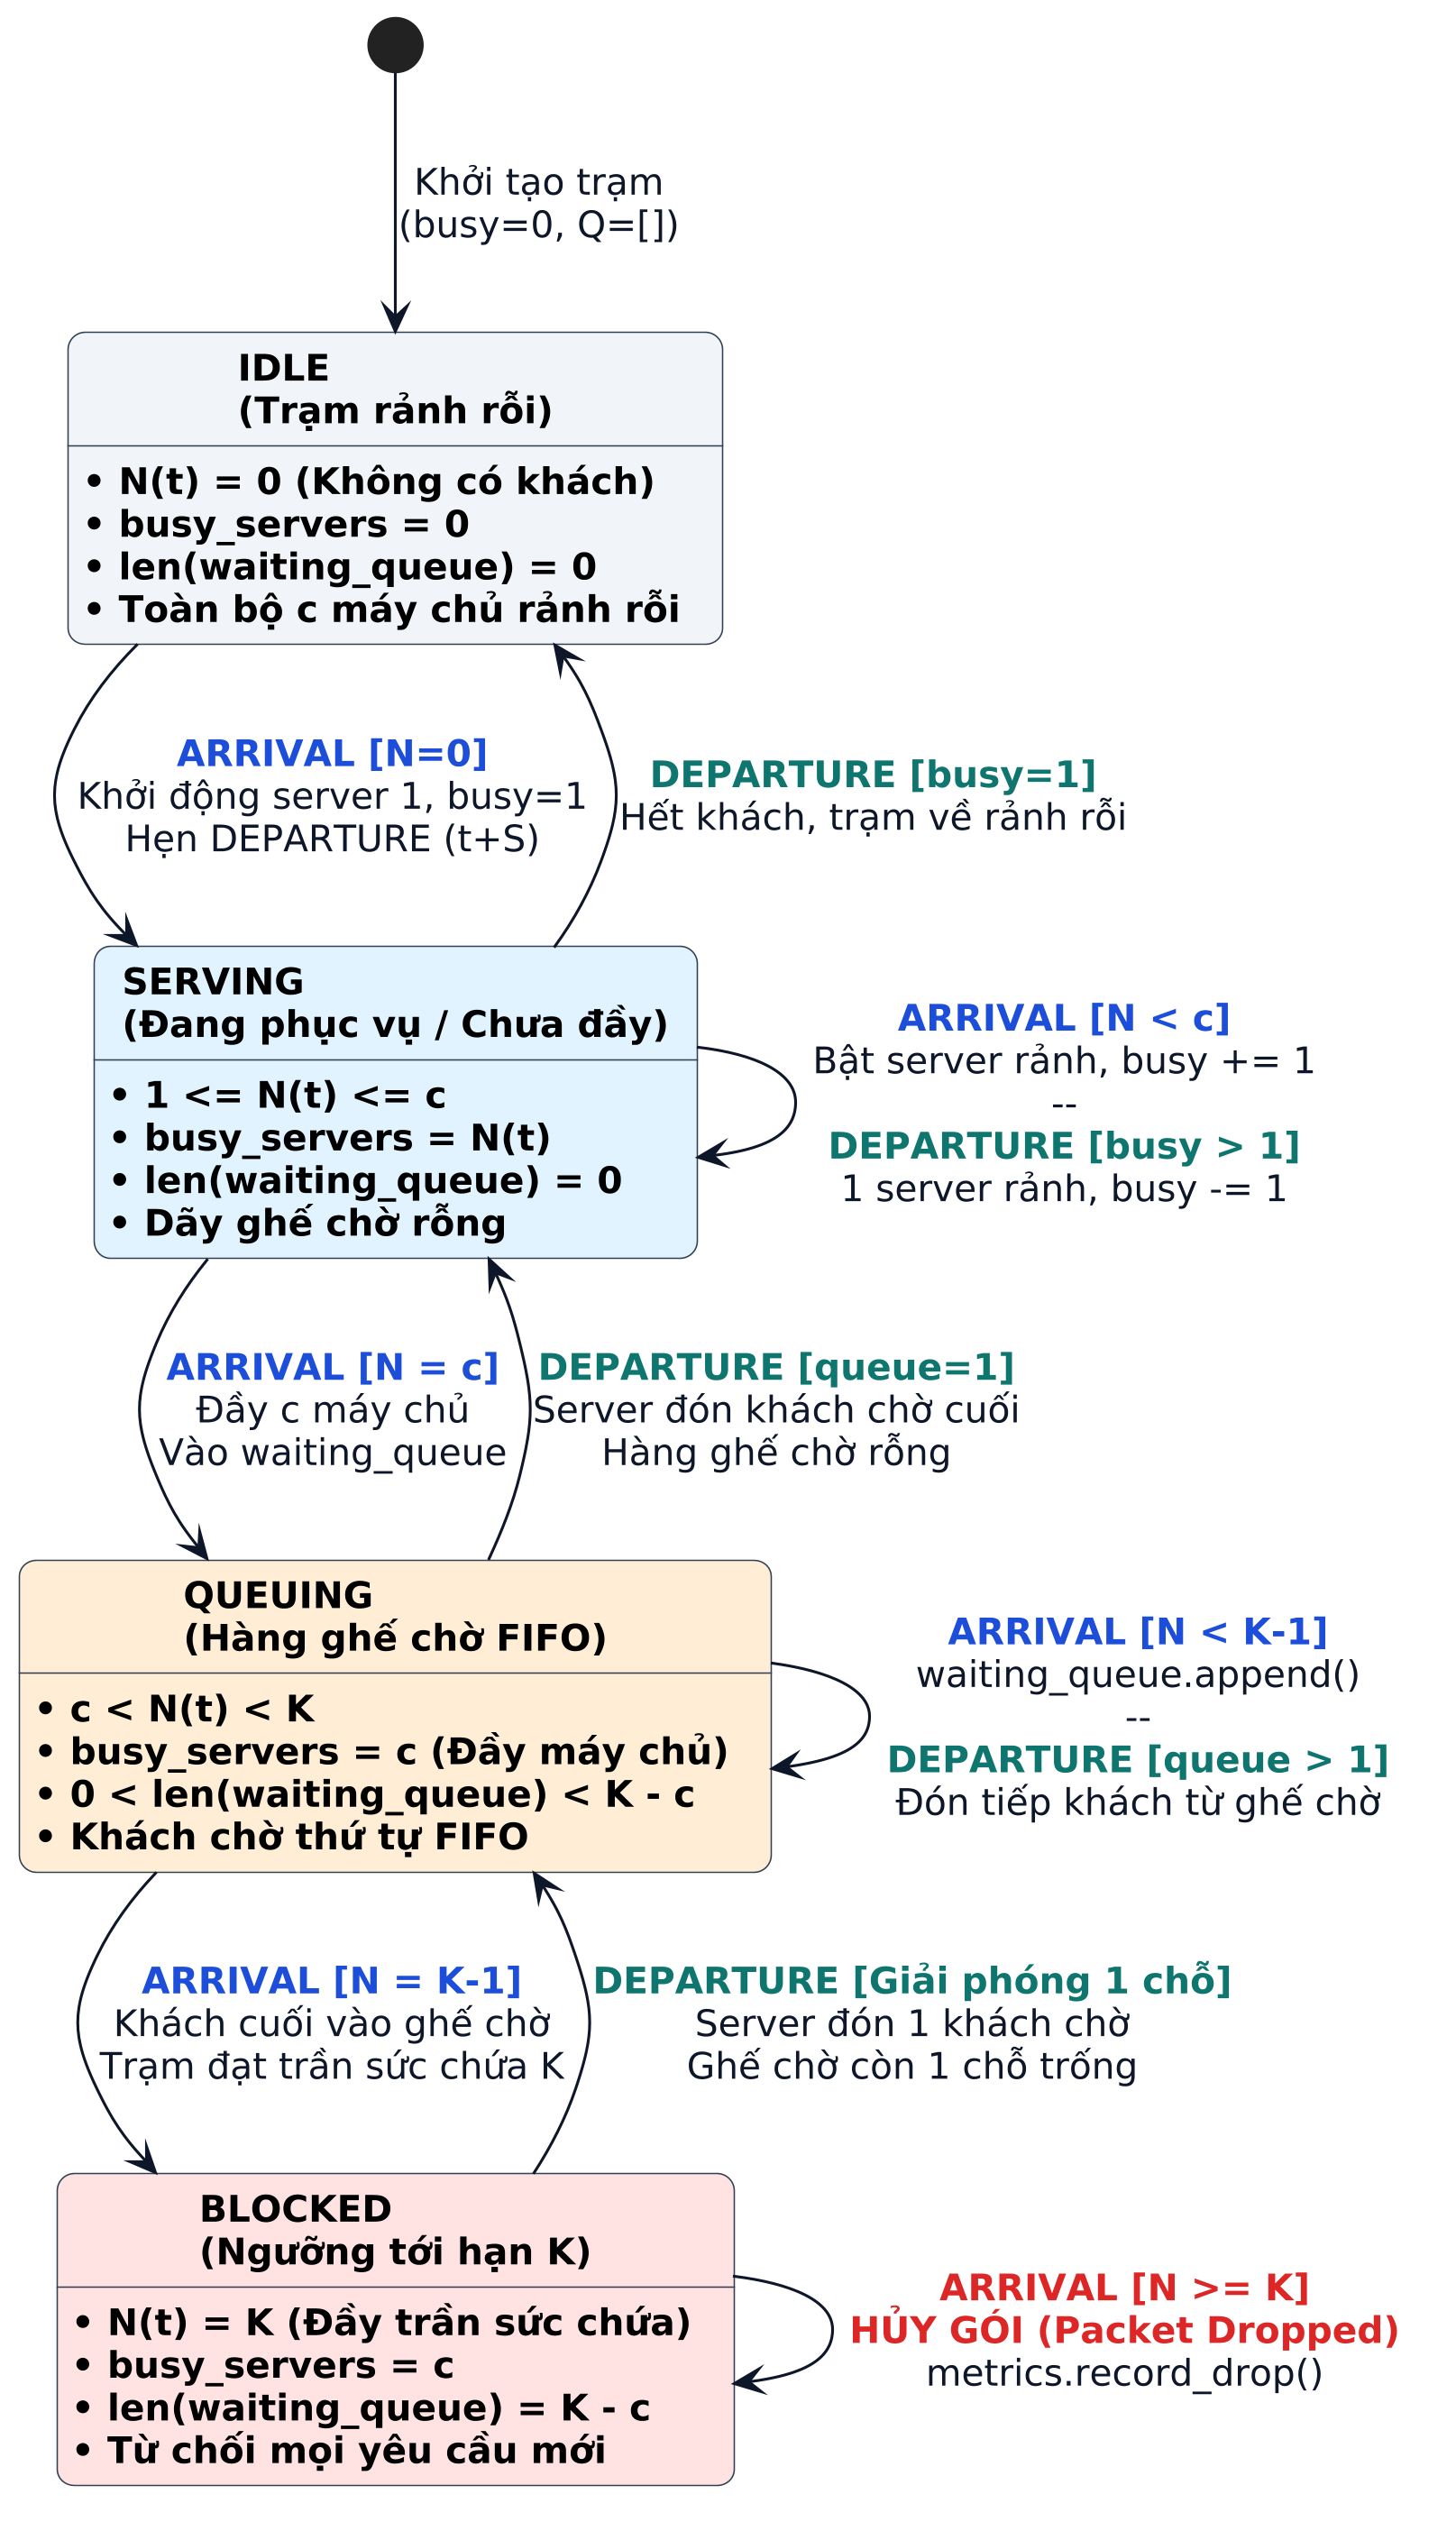
\includegraphics[width=0.6\textwidth]{image/fsm_queue_server_uml.png}
\caption{Máy trạng thái hữu hạn (FSM) mô hình hóa vòng đời phục vụ của \texttt{QueueServerLP}}
\label{fig:fsm-queue-server}
\end{figure}
\begin{itemize}[leftmargin=1.5em, itemsep=3pt]
\item \textbf{Máy trạng thái tiếp nhận (\texttt{\_handle\_arrival}):}
\begin{enumerate}[leftmargin=1.2em, label=\alph*)]
\item \textit{Kiểm tra sức chứa:} Tính tổng số khách trong trạm thông qua thuộc tính \texttt{total\_in\_system}, xác định bởi $N(t) = \text{busy} + |\mathcal{Q}_{\text{wait}}|$. Nếu $N(t) \ge K$ (với cấu hình có bộ đệm hữu hạn), trạm lập tức kích hoạt \texttt{self.metrics.record\_drop()} và hủy gói tin.
\item \textit{Điều phối máy chủ rảnh:} Nếu $\text{busy\_servers} < c$, trạm tăng số máy chủ bận thêm $1$ (\texttt{self.busy\_servers += 1}), bốc thời gian phục vụ $S \sim \text{Exp}(\mu)$ và phát sự kiện \texttt{DEPARTURE} trong tương lai qua \texttt{create\_event} với độ trễ $S$.
\item \textit{Xếp hàng chờ FIFO:} Nếu cả $c$ máy chủ đều bận, yêu cầu được đẩy vào hàng ghế chờ \texttt{waiting\_queue} bằng thao tác \texttt{append} đạt $\mathcal{O}(1)$.
\end{enumerate}
\item \textbf{Máy trạng thái hoàn tất (\texttt{\_handle\_departure}):}
\begin{enumerate}[leftmargin=1.2em, label=\alph*)]
\item \textit{Ghi nhận số liệu thống kê:} Tính thời gian chờ thực tế $W_q = t_{\text{start\_service}} - t_{\text{arrival}}$ và ghi nhận vào bộ tích lũy \texttt{MetricsCollector} qua phương thức \texttt{record\_completion(wait\_time, service\_duration)}.
\item \textit{Chuyển tiếp tác vụ:} Đóng gói đối tượng \texttt{Job} đã hoàn tất và phát sự kiện \texttt{ARRIVAL} tới trạm kế tiếp (\texttt{dest\_lp\_id}) qua \texttt{create\_event} với độ trễ $\Delta t = 0.0$.
\item \textit{Đón khách tiếp theo:} Nếu hàng chờ \texttt{waiting\_queue} còn khách, lấy phần tử đầu hàng qua \texttt{popleft()} ($\mathcal{O}(1)$) và phục vụ ngay. Nếu hàng rỗng, giảm biến đếm máy chủ bận: $\text{busy\_servers} \leftarrow \max(0, \text{busy\_servers} - 1)$.
\end{enumerate}
\end{itemize}

\subsubsection{Hiện thực mạng hàng đợi Jackson và Cơ chế rẽ nhánh xác suất}
\label{subsubsec:jackson-network-impl}

\hspace{0.5cm}Nhằm mô hình hóa mạng máy tính 4 nút trạm phức tạp theo Hình 1 của đề bài ($\text{Source} \to \text{I/O} \to \text{CPU} \to \text{Printer} / \text{Disk} \to \text{Sink}$), lớp \textbf{\texttt{BranchingServerLP}} kế thừa từ \texttt{QueueServerLP} và ghi đè logic hoàn tất phục vụ:

\begin{lstlisting}[language=Python, caption={Hiện thực rẽ nhánh xác suất trong BranchingServerLP (bkitevsim/models/network.py)}, label={lst:branching-server}]
class BranchingServerLP(QueueServerLP):
    """Probabilistic routing server modeling CPU departure branch in Jackson network."""

    def __init__(
        self,
        lp_id: int | str = "CPU",
        printer_lp_id: int | str = "Printer",
        disk_lp_id: int | str = "Disk",
        p_printer: float = 0.3,
        service_rate: float = 5.0,
        num_servers: float = 1,
        capacity: Optional[int] = None,
        metrics: Optional[MetricsCollector] = None
    ) -> None:
        super().__init__(
            lp_id=lp_id,
            dest_lp_id=printer_lp_id,
            service_rate=service_rate,
            num_servers=num_servers,
            capacity=capacity,
            metrics=metrics
        )
        self.printer_lp_id = printer_lp_id
        self.disk_lp_id = disk_lp_id
        self.p_printer = p_printer  # Probability of routing to Printer (0.3)

    def _handle_departure(self, event: Event) -> None:
        """Route departing job probabilistically via Bernoulli trial to Printer or Disk."""
        payload = event.payload if isinstance(event.payload, dict) else {}
        job: Job = payload.get("job")
        service_duration: float = payload.get("duration", 0.0)

        if job and job.start_service_time is not None:
            wait_time = job.start_service_time - job.arrival_time
            self.metrics.record_completion(wait_time, service_duration)
            job.departure_time = event.timestamp

            # Probabilistic routing: Bernoulli trial with probability p_printer
            dest = self.printer_lp_id if (random.random() < self.p_printer) else self.disk_lp_id
            if not hasattr(job, "orig_arrival_time"):
                job.orig_arrival_time = job.arrival_time
            job.arrival_time = event.timestamp

            out_ev = create_event(
                timestamp=event.timestamp,
                sender_id=self.lp_id,
                receiver_id=dest,
                event_type="ARRIVAL",
                payload={"job": job}
            )
            self.send_event(out_ev)

        if self.waiting_queue:
            next_job = self.waiting_queue.popleft()
            self._start_service(next_job, event.timestamp)
        else:
            self.busy_servers = max(0, self.busy_servers - 1)

        self._notify_state(event.timestamp)
\end{lstlisting}

\begin{itemize}[leftmargin=1.5em, itemsep=2pt]
\item \textbf{Cơ chế rẽ nhánh Bernoulli (\texttt{p\_printer}):} Tại ngã ba xuất phát từ CPU, bộ điều phối trạm thực hiện phép thử ngẫu nhiên: nếu $\text{random}() < p_{\text{printer}}$ (mặc định $0.3$) thì chuyển gói tin sang trạm \texttt{PrinterLP}, ngược lại ($1 - p = 0.7$) chuyển sang trạm \texttt{DiskLP}.
\item \textbf{Cơ chế bảo toàn mốc thời gian gốc (\texttt{orig\_arrival\_time}):} Khi gói tin chuyển tiếp qua các trạm I/O $\to$ CPU $\to$ Printer/Disk, thuộc tính \texttt{arrival\_time} được cập nhật tại chỗ để tính cục bộ $W_{q,\text{node}}$, trong khi \texttt{orig\_arrival\_time} được giữ nguyên vẹn giúp trạm đích \texttt{NetworkSinkLP} tính toán chính xác độ trễ toàn trình (\textit{End-to-End Latency}):
\begin{equation}
T_{\text{End-to-End}} = t_{\text{Sink}} - \text{job.orig\_arrival\_time}
\end{equation}
giúp đối chiếu trực tiếp với định lý Jackson giải tích: $W_{\text{network}} = W_{\text{IO}} + W_{\text{CPU}} + 0.3 W_{\text{Printer}} + 0.7 W_{\text{Disk}}$.
\end{itemize}

% =========================================================================
\subsection{Cơ chế giao tiếp phi nghẽn và Điều phối bất đồng bộ (Python Asyncio)}
\label{subsec:asyncio-implementation}
% =========================================================================

\subsubsection{Cơ chế giao tiếp phi nghẽn luồng theo mô hình Promise / Future}
\label{subsubsec:promise-future}

\hspace{0.5cm}Để kết nối giữa luồng gọi người dùng và bộ máy mô phỏng mà không gây nghẽn luồng chính (\textit{Non-blocking I/O}), lớp \textbf{\texttt{AsyncFutureManager}} hiện thực mẫu thiết kế Promise/Future:
\begin{itemize}[leftmargin=1.5em, itemsep=2pt]
\item \textbf{Khởi tạo và Quản lý Event Loop an toàn (\texttt{\_get\_loop}):} Tự động phát hiện vòng lặp sự kiện \texttt{asyncio} đang chạy hoặc tạo mới an toàn trên các phiên bản Python 3.10+, 3.11+ và 3.12+, tránh hoàn toàn lỗi \texttt{RuntimeError: no running event loop}.
\item \textbf{Tạo lời hứa (\texttt{create\_future}):} Khởi tạo một đối tượng \texttt{asyncio.Future} được gán nhãn duy nhất theo \texttt{request\_id} và lưu vào bảng tra cứu \texttt{\_pending\_futures}. Luồng gọi coroutine phía người dùng có thể thực hiện toán tử \texttt{await future} để tạm dừng tác vụ một cách hòa nhã mà không chiếm dụng CPU.
\item \textbf{Giải phóng lời hứa (\texttt{set\_result}):} Khi trạm thu gom \texttt{SinkLP} tiếp nhận kết quả cuối cùng của yêu cầu, phương thức \texttt{set\_result(request\_id, result)} lập tức hoàn tất Future và đánh thức coroutine đang chờ để nhận kết quả ngay tức thời.
\item \textbf{Báo lỗi và Hủy an toàn (\texttt{set\_exception}, \texttt{cancel\_all}):} Cho phép truyền trực tiếp đối tượng ngoại lệ vào Future khi gặp sự cố, hoặc hủy bỏ hàng loạt các lời hứa đang treo khi dừng hệ thống.
\end{itemize}

\begin{lstlisting}[language=Python, caption={Cơ chế Promise / Future phi nghẽn (bkitevsim/async\_engine/future\_manager.py)}, label={lst:future-manager}]
class AsyncFutureManager:
    """Manages asynchronous Request-to-Future lifecycle without thread blocking."""

    def __init__(self, loop: Optional[asyncio.AbstractEventLoop] = None) -> None:
        self.loop = loop
        # Pending future registry: mapping request_id -> asyncio.Future
        self._pending_futures: Dict[int, asyncio.Future] = {}

    def _get_loop(self) -> asyncio.AbstractEventLoop:
        """Retrieve active running event loop or create a fresh loop safely."""
        if self.loop is not None and not self.loop.is_closed():
            return self.loop
        try:
            return asyncio.get_running_loop()
        except RuntimeError:
            loop = asyncio.new_event_loop()
            asyncio.set_event_loop(loop)
            self.loop = loop
            return loop

    def create_future(self, request_id: int) -> asyncio.Future:
        """Create and register an asyncio.Future attached to a unique request ID."""
        loop = self._get_loop()
        future = loop.create_future()
        self._pending_futures[request_id] = future
        return future

    def set_result(self, request_id: int, result: Any) -> bool:
        """Resolve promise with result, awakening awaiting coroutine."""
        future = self._pending_futures.pop(request_id, None)
        if future and not future.done():
            future.set_result(result)
            return True
        return False
\end{lstlisting}

\subsubsection{Các mẫu điều phối đồng quy có cấu trúc (Structured Concurrency)}
\label{subsubsec:structured-concurrency}

\hspace{0.5cm}Từ phiên bản Python 3.11+, cơ chế \textbf{Structured Concurrency} qua \texttt{asyncio.TaskGroup} được áp dụng để quản lý an toàn vòng đời coroutine. Lớp \textbf{\texttt{AsyncTaskCoordinator}} chuẩn hóa 4 mẫu điều phối:

\begin{enumerate}[leftmargin=2em, itemsep=3pt]
\item \textbf{Mẫu TaskGroup (\texttt{run\_with\_task\_group}):} Quản lý các coroutine con trong ngữ cảnh \texttt{async with asyncio.TaskGroup()}. Khi có một tác vụ con gặp ngoại lệ, toàn bộ các tác vụ còn lại sẽ được hủy tự động, loại trừ nguy cơ rò rỉ tác vụ (\textit{Task Leak}).
\item \textbf{Mẫu Gom nhóm song hành (\texttt{run\_with\_gather}):} Kích hoạt đồng thời danh sách các coroutine và đợi kết quả tổng thể với \texttt{asyncio.gather}.
\item \textbf{Mẫu Tiêu thụ FCFS (\texttt{process\_as\_completed}):} Xử lý kết quả theo nguyên tắc Đến trước -- Phục vụ trước với \texttt{asyncio.as\_completed}. Bất kỳ tác vụ nào xong trước sẽ được chuyển ngay cho hàm callback.
\item \textbf{Mẫu Runner cô lập (\texttt{run\_in\_runner}):} Sử dụng \texttt{asyncio.Runner()} để thiết lập Event Loop độc lập cho mỗi đợt mô phỏng, bảo đảm dọn dẹp sạch tài nguyên hệ điều hành sau khi hoàn thành.
\end{enumerate}

\begin{lstlisting}[language=Python, caption={4 mẫu điều phối bất đồng bộ chuẩn mực (bkitevsim/async\_engine/task\_coordinator.py)}, label={lst:task-coordinator}]
class AsyncTaskCoordinator:
    """Orchestrates concurrent simulation execution (Section 4 specifications)."""

    @staticmethod
    async def run_with_task_group(
        coroutines: Sequence[Coroutine[Any, Any, Any]]
    ) -> List[Any]:
        """Listing 2b: Structured concurrency via asyncio.TaskGroup (Python 3.11+)."""
        tasks = []
        async with asyncio.TaskGroup() as tg:
            for coro in coroutines:
                task = tg.create_task(coro)
                tasks.append(task)
        return [task.result() for task in tasks]

    @staticmethod
    async def run_with_gather(
        coroutines: Sequence[Coroutine[Any, Any, Any]]
    ) -> List[Any]:
        """Listing 2a: Unscoped concurrent execution using asyncio.gather."""
        return await asyncio.gather(*coroutines)

    @staticmethod
    async def process_as_completed(
        coroutines: Sequence[Coroutine[Any, Any, Any]],
        callback: Callable[[Any], None]
    ) -> List[Any]:
        """Listing 2c: Streaming results in FCFS order using as_completed."""
        results = []
        for finished_task in asyncio.as_completed(coroutines):
            result = await finished_task
            callback(result)
            results.append(result)
        return results

    @staticmethod
    def run_in_runner(main_coro: Coroutine[Any, Any, Any]) -> Any:
        """Listing 3a(bis): Program entry point with isolated asyncio.Runner."""
        with asyncio.Runner() as runner:
            return runner.run(main_coro)
\end{lstlisting}

% Bảng~\ref{tab:async-patterns-comparison} tổng kết sự so sánh đặc tính kỹ thuật và kịch bản ứng dụng của 4 mẫu điều phối bất đồng bộ trong \texttt{AsyncTaskCoordinator}.

\begin{table}[H]
\centering
\small
\renewcommand{\arraystretch}{1.35}
\setlength{\tabcolsep}{5pt}
\setlength{\aboverulesep}{0pt}
\setlength{\belowrulesep}{0pt}
\noindent\begin{tabularx}{\linewidth}{>{\ttfamily\bfseries\color{bkblue}\raggedright\arraybackslash}p{2.6cm} >{\centering\arraybackslash}p{2.0cm} >{\raggedright\arraybackslash}X >{\raggedright\arraybackslash}X}
\arrayrulecolor{bkblue}\toprule[1.5pt]
\rowcolor{bkblue}%
\multicolumn{1}{>{\raggedright\arraybackslash}p{2.6cm}}{\textbf{\color{white}Mẫu điều phối}} &
\multicolumn{1}{>{\centering\arraybackslash}p{2.0cm}}{\textbf{\color{white}Phạm vi}} &
\multicolumn{1}{>{\raggedright\arraybackslash}X}{\textbf{\color{white}Cơ chế quản lý ngoại lệ}} &
\multicolumn{1}{>{\raggedright\arraybackslash}X}{\textbf{\color{white}Kịch bản ứng dụng tối ưu}} \\
\midrule[1pt]
\rowcolor{white}TaskGroup & Scoped & Tự động hủy tác vụ còn lại nếu xảy ra lỗi (\textit{Fail-fast}) & Chạy nhóm mô phỏng ràng buộc nghiệp vụ liên đới \\
\rowcolor{boxbg}gather & Unscoped & Trả về danh sách ngoại lệ hoặc hủy thủ công qua task handle & Chạy song song các bộ tham số hoàn toàn độc lập \\
\rowcolor{white}as\_completed & Streaming & Xử lý ngay khi tác vụ hoàn tất theo thứ tự FCFS & Bơm trực tiếp dữ liệu ra dashboard theo thời gian thực \\
\rowcolor{boxbg}Runner & Isolated & Khởi tạo và đóng Event Loop độc lập tuyệt đối & Chạy các bài kiểm thử tự động (\textit{Unit / Integration Test}) \\
\arrayrulecolor{bkblue}\bottomrule[1.5pt]
\end{tabularx}
\caption{So sánh đặc tính kỹ thuật của 4 mẫu điều phối bất đồng bộ}
\label{tab:async-patterns-comparison}
\end{table}

\newpage
% =========================================================================
\subsection{Quản lý thời gian ảo và Kiểm chứng tính nhân quả cục bộ}
\label{subsec:simulation-vs-wallclock}
% =========================================================================

\subsubsection{Nguyên lý bước nhảy thời gian ảo và Phân tách với thời gian thực}
\label{subsubsec:virtual-clock-jump}

\hspace{0.5cm}Sự phân tách tuyệt đối giữa \textbf{Thời gian ảo mô phỏng (\textit{Virtual Simulation Time})} và \textbf{Thời gian thực máy tính (\textit{Wall-clock Time})} là nguyên lý cốt lõi của công nghệ DES.

\begin{tcolorbox}[colback=red!5!white, colframe=red!75!black, title=\textbf{Cảnh báo sai lầm nghiêm trọng trong mô phỏng DES}]
Tuyệt đối không được dùng lệnh \texttt{time.sleep()} hoặc \texttt{asyncio.sleep()} để mô phỏng độ trễ phục vụ. Việc dùng lệnh sleep sẽ trói buộc thời gian ảo vào chu kỳ xung nhịp vật lý của CPU, khiến cuộc thử nghiệm $10.000$ giây ảo đòi hỏi máy tính thực tế phải chờ gần 3 giờ đồng hồ.
\end{tcolorbox}

Trong bộ mô phỏng của nhóm:
\begin{itemize}[leftmargin=1.5em, itemsep=2pt]
\item Đồng hồ \texttt{dispatcher.current\_time} thực hiện \textbf{bước nhảy gián đoạn (jump)} thẳng tới timestamp của sự kiện kế tiếp trong hàng đợi.
\item Các khoảng thời gian hệ thống rảnh rỗi (\textit{idle}) hoặc khách ngồi đợi trong hàng ghế không tiêu tốn chu kỳ CPU thực tế.
\item Một kịch bản thử nghiệm quy mô lớn với $50.000$ sự kiện kéo dài $5000$ giây ảo được hoàn tất chỉ trong khoảng $0.2 \to 0.4$ giây thực tế máy tính.
\end{itemize}

Bảng~\ref{tab:sim-paradigm-comparison} phân định rạch ròi sự khác biệt bản chất giữa mô phỏng sự kiện rời rạc và mô phỏng theo nhịp xung thời gian thực.

\begin{table}[H]
\centering
\small
\renewcommand{\arraystretch}{1.35}
\setlength{\tabcolsep}{5pt}
\setlength{\aboverulesep}{0pt}
\setlength{\belowrulesep}{0pt}
\noindent\begin{tabularx}{\linewidth}{>{\raggedright\arraybackslash\bfseries\color{bkblue}}p{3.2cm} >{\raggedright\arraybackslash}X >{\raggedright\arraybackslash}X}
\arrayrulecolor{bkblue}\toprule[1.5pt]
\rowcolor{bkblue}%
\multicolumn{1}{>{\raggedright\arraybackslash}p{3.2cm}}{\textbf{\color{white}Tiêu chí kỹ thuật}} &
\multicolumn{1}{>{\raggedright\arraybackslash}X}{\textbf{\color{white}Mô phỏng DES (Hệ thống đề tài)}} &
\multicolumn{1}{>{\raggedright\arraybackslash}X}{\textbf{\color{white}Mô phỏng thời gian thực (Real-time)}} \\
\midrule[1pt]
\rowcolor{white}Bước nhảy thời gian & Gián đoạn theo sự kiện: $t_{k+1} = e_{\text{next}}.\text{timestamp}$ & Tuyến tính theo chu kỳ cố định $\Delta t$ hoặc lệnh \texttt{sleep()} \\
\rowcolor{boxbg}Hiệu suất CPU & Tối đa $100\%$, bỏ qua hoàn toàn các khoảng thời gian rảnh rỗi & Lãng phí chu kỳ xung nhịp chờ lệnh \texttt{sleep()} nhả khóa \\
\rowcolor{white}Tốc độ mô phỏng & Nhanh hơn thực tế hàng nghìn lần ($5000$s ảo $\approx 0.3$s thực) & Bị neo chặt vào thời gian vật lý thực ($5000$s ảo $\approx 5000$s thực) \\
\rowcolor{boxbg}Độ chính xác thời gian & Chính xác số học tuyệt đối theo phân phối ngẫu nhiên & Bị sai lệch do độ trễ điều phối luồng (\textit{OS Thread Jitter}) \\
\arrayrulecolor{bkblue}\bottomrule[1.5pt]
\end{tabularx}
\caption{So sánh bản chất giữa Mô phỏng DES và Mô phỏng theo thời gian thực}
\label{tab:sim-paradigm-comparison}
\end{table}

\subsubsection{Ràng buộc nhân quả cục bộ và Kiểm chứng vết tính toán}
\label{subsubsec:causality-verification}

Để kết quả mô phỏng có giá trị khoa học, chuỗi tiến trình phải tuân thủ nghiêm ngặt \textbf{Ràng buộc nhân quả cục bộ (\textit{Local Causality Constraint})}:
\begin{equation}
t_{\text{current}}^{(1)} \le t_{\text{current}}^{(2)} \le \dots \le t_{\text{current}}^{(M)}
\end{equation}

\paragraph{Chứng minh tính bảo toàn nhân quả trong hạt nhân điều phối:}
Tính bất biến nhân quả $t_{\text{current}}^{(n+1)} \ge t_{\text{current}}^{(n)}$ được bảo đảm tuyệt đối nhờ hai tiền đề toán học:
\begin{itemize}[leftmargin=1.5em, itemsep=2pt]
\item \textbf{Tiền đề trật tự Min-Heap:} Hàng đợi sự kiện $\mathcal{Q}$ luôn trả về phần tử có $\text{timestamp}$ nhỏ nhất: $e_{\text{next}} = \min_{e \in \mathcal{Q}}(e.\text{timestamp})$. Do đó, $e_{\text{next}}.\text{timestamp} \ge t_{\text{current}}$.
\item \textbf{Tiền đề độ trễ không âm:} Mọi sự kiện phát sinh mới trong tương lai đều có độ trễ $\Delta t \ge 0$, tức là $t_{\text{new}} = t_{\text{current}} + \Delta t \ge t_{\text{current}}$. Không một tiến trình nào có thể gửi thông điệp về quá khứ ($\Delta t < 0$).
\end{itemize}
Từ hai tiền đề trên, theo phương pháp quy nạp toán học, chuỗi thời gian ảo của vòng lặp điều phối luôn là một dãy đơn điệu tăng ngặt trên trục thời gian, loại trừ hoàn toàn nguy cơ vi phạm nhân quả (\textit{Causality Violation}).

Hệ thống bảo đảm tính đơn điệu này qua 2 lớp phòng vệ thực tiễn:
\begin{enumerate}[leftmargin=2em, itemsep=3pt]
\item \textbf{Phòng vệ nội tại tại từng LP (\texttt{set\_local\_virt\_time}):} Nếu một sự kiện nổ ra có timestamp nhỏ hơn LVT hiện tại của trạm, phương thức lập tức ném ngoại lệ \texttt{ValueError("Causality violation in LP...")} và ngắt tiến trình để bảo toàn tính toàn vẹn của thời gian ảo.
\item \textbf{Kiểm chứng tự động trên vết thực thi (\texttt{trace\_log}):} Toàn bộ các sự kiện được ghi nhận vào nhật ký vết tính toán và được kiểm chứng tự động qua bộ test suite chính quy trong tệp \texttt{tests/test\_verification.py}:
\begin{itemize}[leftmargin=1.5em, itemsep=2pt]
\item \texttt{test\_causality\_trace\_analysis()}: Kiểm tra tính đơn điệu tăng ngặt của trục thời gian ảo trên toàn bộ vết sự kiện được ghi nhận bởi Dispatcher.
\item \texttt{test\_priority\_queue\_monotonicity()}: Kiểm tra thứ tự trích xuất sự kiện luôn đơn điệu tăng trên cả \texttt{MinHeapPriorityQueue} và \texttt{LadderQueue}.
\item \texttt{test\_event\_conservation\_law()}: Kiểm chứng định luật bảo toàn biến cố: tổng số gói tin đến bằng tổng số gói tin phục vụ xong cộng số gói tin bị rớt do tràn bộ đệm.
\end{itemize}
\end{enumerate}



\clearpage

% \section{Kịch bản thực nghiệm, Kiểm chứng và Thẩm định}
\label{sec:thuc-nghiem-vv}

\textit{\textbf{Hướng dẫn chung cho Phần 4:}} Đây là phần chiếm trọng số điểm cao nhất (Giai đoạn 2 -- 4 điểm). Nhóm cần trình bày đầy đủ các kịch bản thực nghiệm, phân biệt rõ giữa Kiểm chứng (Verification -- kiểm tra code chạy đúng logic) và Thẩm định (Validation -- kiểm tra mô hình khớp với lý thuyết toán học), kèm theo phân tích độ nhạy và nhận diện điểm nghẽn.

\subsection{Thiết kế khối lượng công việc (Workload)}
\label{subsec:workload-design}

\subsubsection{Bộ sinh tải Poisson và Exponential}
\textit{\textbf{Nội dung cần viết:}}
\begin{itemize}[leftmargin=1.5em]
    \item Trình bày phương pháp nghịch đảo hàm phân phối tích lũy (\textit{Inverse Transform Sampling}) để sinh biến ngẫu nhiên thời gian đến và thời gian phục vụ:
    \begin{equation}
        X = -\frac{1}{\lambda} \ln(1 - U) \quad \text{với } U \sim \text{Uniform}(0, 1)
    \end{equation}
    \item Vẽ biểu đồ tần suất (Histogram) so sánh phân phối mẫu được sinh ra với hàm mật độ xác suất lý thuyết $f(x) = \lambda e^{-\lambda x}$ để chứng minh tính chuẩn xác của bộ sinh tải.
\end{itemize}

\subsubsection{Kịch bản tải biến động ngẫu nhiên (Bursty Traffic)}
\textit{\textbf{Nội dung cần viết:}}
\begin{itemize}[leftmargin=1.5em]
    \item Thiết kế kịch bản tải đột biến (Traffic Burst) theo từng đợt để kiểm tra độ bền và khả năng hấp thụ tải của các mô hình hàng đợi có bộ đệm.
\end{itemize}

\subsection{Thiết kế kịch bản thực nghiệm (Experimental Design)}
\label{subsec:experimental-design}

\subsubsection{Ma trận kịch bản đo đạc}
\textit{\textbf{Nội dung cần viết:}}
Lập bảng ma trận các kịch bản thử nghiệm cho từng mô hình:
\begin{itemize}[leftmargin=1.5em]
    \item \textbf{Mô hình $M/M/1$ \& $M/M/c$:} Cố định $\mu = 10$, quét $\lambda$ từ $1$ đến $9.5$ (tương ứng $\rho \in [0.1, 0.95]$).
    \item \textbf{Mô hình $M/M/1/K$ \& $M/M/c/K$:} Quét $K \in \{5, 10, 20, 50\}$ dưới các mức tải $\rho \in \{0.5, 0.8, 1.0, 1.2\}$ (khảo sát cả trường hợp quá tải $\rho \ge 1$).
    \item \textbf{Mô hình Erlang loss $M/M/n/n$:} Khảo sát số kênh $n \in \{2, 5, 10, 20\}$, thay đổi tải Erlang $a = \lambda/\mu$ từ $1$ đến $15$.
    \item \textbf{Mạng hàng đợi (Network):} Cấu hình các tham số theo Hình 1 đề bài: $\mu_4$ (I/O), $\mu_1$ (CPU), $\mu_2$ (Printer), $\mu_3$ (Disk) với xác suất rẽ nhánh $p_{printer}=0.3$, $p_{disk}=0.7$.
    \item Thời gian chạy mô phỏng: Tối thiểu $T_{sim} = 10{,}000$ đơn vị thời gian hoặc xử lý tối thiểu $100{,}000$ sự kiện để đạt trạng thái dừng (\textit{steady-state}).
\end{itemize}

\subsubsection{Chiến lược lặp (Replications) và Khoảng tin cậy 95\%}
\textit{\textbf{Nội dung cần viết:}}
\begin{itemize}[leftmargin=1.5em]
    \item Áp dụng kỹ thuật chạy lặp độc lập (\textit{Independent Replications}): Chạy mỗi kịch bản ít nhất $R = 30$ lần với các giá trị \texttt{seed} ngẫu nhiên khác nhau.
    \item Tính giá trị trung bình mẫu $\bar{X}$, độ lệch chuẩn mẫu $s$ và khoảng tin cậy 95\% theo phân phối Student's $t$:
    \begin{equation}
        CI_{95\%} = \left[ \bar{X} - t_{0.975, R-1} \frac{s}{\sqrt{R}}, \quad \bar{X} + t_{0.975, R-1} \frac{s}{\sqrt{R}} \right]
    \end{equation}
    \item Đảm bảo vẽ các thanh sai số (\textit{error bars}) trên toàn bộ đồ thị kết quả thực nghiệm.
\end{itemize}

\subsection{Kiểm chứng mã nguồn mô phỏng (Verification)}
\label{subsec:verification}

\subsubsection{Kiểm thử đơn vị các thành phần (Component Unit Testing)}
\textit{\textbf{Nội dung cần viết:}}
\begin{itemize}[leftmargin=1.5em]
    \item Trình bày các ca kiểm thử tự động (\texttt{pytest}): Test thứ tự ưu tiên của \texttt{LadderQueue}, test xử lý push/pop không làm mất sự kiện, test logic giải phóng server khi hoàn thành tác vụ.
\end{itemize}

\subsubsection{Phân tích nhật ký vết tính toán (Computational Trace Analysis)}
\textit{\textbf{Nội dung cần viết:}}
\begin{itemize}[leftmargin=1.5em]
    \item Trích xuất nhật ký vết (trace log) của 20 sự kiện liên tiếp đầu tiên.
    \item Phân tích chứng minh dấu thời gian luôn tăng đơn điệu ($t_1 \le t_2 \le \dots \le t_{20}$), không xảy ra hiện tượng sự kiện tương lai can thiệp vào quá khứ.
\end{itemize}

\subsubsection{Kiểm tra tính nhất quán logic}
\textit{\textbf{Nội dung cần viết:}}
\begin{itemize}[leftmargin=1.5em]
    \item Kiểm tra định luật bảo toàn số lượng yêu cầu:
    \begin{equation}
        N_{arrived} = N_{completed} + N_{in\_system} + N_{dropped}
    \end{equation}
    Sai số bảo toàn phải tuyệt đối bằng 0 trong toàn bộ các đợt mô phỏng.
\end{itemize}

\subsection{Thẩm định mô hình thực nghiệm (Validation)}
\label{subsec:validation}

\textit{\textbf{Yêu cầu cốt lõi:}} Với mỗi mô hình bên dưới, bắt buộc phải có: (1) Bảng đối chiếu số liệu [Lý thuyết vs Mô phỏng vs Sai số \%], (2) Đồ thị so sánh trực quan (đường lý thuyết nét liền, điểm mô phỏng dạng chấm có thanh sai số).

\subsubsection{Thẩm định mô hình hàng đợi đơn \texorpdfstring{$M/M/1$}{M/M/1}}
\textit{\textbf{Nội dung cần viết:}}
\begin{itemize}[leftmargin=1.5em]
    \item Lập bảng và vẽ đồ thị so sánh $L$ và $W$ giữa mô phỏng và công thức $L = \frac{\rho}{1-\rho}$, $W = \frac{1}{\mu - \lambda}$.
    \item Chứng minh sai số tương đối $\text{Error} = \frac{|\text{Sim} - \text{Theory}|}{\text{Theory}} \times 100\% < 3\%$.
\end{itemize}

\subsubsection{Thẩm định mô hình hàng đợi hữu hạn \texorpdfstring{$M/M/1/K$}{M/M/1/K} và \texorpdfstring{$M/M/c/K$}{M/M/c/K}}
\textit{\textbf{Nội dung cần viết:}}
\begin{itemize}[leftmargin=1.5em]
    \item So sánh xác suất rớt gói $P_b$ và thông lượng thực tế $\lambda_{eff}$ giữa mô phỏng và công thức giải tích.
\end{itemize}

\subsubsection{Thẩm định hệ thống mất gói \texorpdfstring{$M/M/n/n$}{M/M/n/n} (Erlang-B)}
\textit{\textbf{Nội dung cần viết:}}
\begin{itemize}[leftmargin=1.5em]
    \item Vẽ đồ thị so sánh xác suất chặn $P_b$ thu thập từ mô phỏng với đường cong lý thuyết \textbf{Erlang-B} khi thay đổi tải Erlang $a \in [1, 20]$.
\end{itemize}

\subsubsection{Thẩm định mô hình đa server \texorpdfstring{$M/M/c$}{M/M/c} (Erlang-C)}
\textit{\textbf{Nội dung cần viết:}}
\begin{itemize}[leftmargin=1.5em]
    \item Đối chiếu xác suất khách hàng phải chờ trong hàng đợi $P(W > 0)$ với công thức \textbf{Erlang-C}.
\end{itemize}

\subsubsection{Thẩm định mô hình mạng hàng đợi (Queuing Network)}
\textit{\textbf{Nội dung cần viết:}}
\begin{itemize}[leftmargin=1.5em]
    \item So sánh thông lượng đo được tại từng nút (I/O, CPU, Printer, Disk) với phương trình cân bằng lưu lượng.
    \item Kiểm chứng tổng thời gian trễ toàn mạng bằng định luật Little mở rộng: $L_{network} = \lambda W_{total}$.
\end{itemize}

\subsection{Phân tích độ nhạy và Tối ưu hóa hệ thống}
\label{subsec:sensitivity-tuning}

\subsubsection{Khảo sát hành vi hệ thống khi tiến đến điểm bão hòa (\texorpdfstring{$\rho \to 1$}{rho -> 1})}
\textit{\textbf{Nội dung cần viết:}}
\begin{itemize}[leftmargin=1.5em]
    \item Phân tích hiện tượng bùng nổ độ trễ và chiều dài hàng đợi khi hệ số tải vượt ngưỡng $\rho = 0.85$.
    \item Xác định điểm giới hạn vận hành tối ưu (knee point) để đảm bảo thông lượng tối đa mà độ trễ vẫn nằm trong ngưỡng chấp nhận được.
\end{itemize}

\subsubsection{Phân tích độ nhạy của dung lượng bộ đệm \texorpdfstring{$K$}{K}}
\textit{\textbf{Nội dung cần viết:}}
\begin{itemize}[leftmargin=1.5em]
    \item Đánh giá sự đánh đổi (\textit{trade-off}): Tăng $K$ giúp giảm tỉ lệ mất gói $P_b$, nhưng lại làm tăng thời gian chờ trung bình $W_q$ (hiện tượng \textit{Bufferbloat}).
    \item Tìm kích thước bộ đệm tối ưu $K^*$ thỏa mãn điều kiện ràng buộc về tỉ lệ mất gói ($P_b \le 1\%$).
\end{itemize}

\subsubsection{Nhận diện nút thắt cổ chai (Bottlenecks) trong mạng hàng đợi}
\textit{\textbf{Nội dung cần viết:}}
\begin{itemize}[leftmargin=1.5em]
    \item Xác định nút có hệ số sử dụng cao nhất trong mạng (ví dụ: nút CPU hoặc Disk).
    \item Phân tích ảnh hưởng của nút thắt cổ chai đến thông lượng tối đa của toàn bộ mạng hệ thống.
\end{itemize}

\subsubsection{Đề xuất phương án tối ưu hóa và phân bổ tài nguyên}
\textit{\textbf{Nội dung cần viết:}}
\begin{itemize}[leftmargin=1.5em]
    \item Đề xuất các giải pháp kỹ thuật: Nâng cấp tốc độ phục vụ $\mu$ của nút nghẽn, bổ sung máy chủ song song tại nút nghẽn, hoặc điều chỉnh tỉ lệ phân luồng ($p_{printer}, p_{disk}$) để cân bằng tải.
    \item Chạy lại mô phỏng sau khi tối ưu hóa để chứng minh hiệu quả cải thiện thông lượng và giảm độ trễ.
\end{itemize}

% \clearpage

% \section{Kết luận và Hướng dẫn sử dụng}
\label{sec:ket-luan}

\textit{\textbf{Hướng dẫn chung cho Phần 5:}} Phần này tổng kết toàn bộ kết quả nghiên cứu, đánh giá mức độ hoàn thành so với mục tiêu ban đầu, rút ra bài học kinh nghiệm và cung cấp tài liệu hướng dẫn sử dụng (User Manual) chi tiết giúp người chấm bài hoặc nhóm đánh giá chéo (Phase 3) có thể tái lập kết quả một cách dễ dàng.

\subsection{Tổng kết kết quả đạt được}
\label{subsec:tong-ket}
\textit{\textbf{Nội dung cần viết:}}
\begin{itemize}[leftmargin=1.5em]
    \item Tóm tắt các thành tựu chính của đề tài:
    \begin{itemize}
        \item Đã xây dựng thành công bộ máy mô phỏng sự kiện rời rạc (DES Core) hỗ trợ quản lý sự kiện bằng hàng đợi ưu tiên \texttt{LadderQueue} và điều phối bất đồng bộ với Python \texttt{asyncio}.
        \item Đã mô hình hóa và kiểm chứng chính xác 6 mô hình hàng đợi kinh điển ($M/M/1$, $M/M/1/K$, $M/M/\infty$, $M/M/n/n$, $M/M/c$, $M/M/c/K$) và 1 mô hình mạng hàng đợi đa chặng.
        \item Độ sai lệch giữa kết quả mô phỏng và công thức giải tích lý thuyết (Little's Law, Erlang-B, Erlang-C) đều nằm trong khoảng tin cậy 95\% với sai số tương đối dưới 3\%.
        \item Nhận diện thành công nút thắt cổ chai trong mạng và đề xuất giải pháp tối ưu hóa năng lực phục vụ.
    \end{itemize}
\end{itemize}

\subsection{Bài học kinh nghiệm và Hướng phát triển}
\label{subsec:bai-hoc-phat-trien}

\subsubsection{Bài học kinh nghiệm trong mô phỏng hệ thống}
\textit{\textbf{Nội dung cần viết:}}
\begin{itemize}[leftmargin=1.5em]
    \item Bài học về việc phân tách tuyệt đối giữa thời gian ảo mô phỏng (\textit{Simulation Virtual Time}) và thời gian thực máy tính (\textit{Wall-clock Time}).
    \item Kinh nghiệm xử lý đồng bộ và tính nhân quả khi kết hợp coroutine bất đồng bộ (\texttt{TaskGroup}, \texttt{Future}) với vòng lặp sự kiện rời rạc.
    \item Tầm quan trọng của việc thu thập đủ số lượng mẫu (Replications) và loại bỏ giai đoạn khởi động (warm-up period) để đạt trạng thái dừng.
\end{itemize}

\subsubsection{Hạn chế và hướng mở rộng}
\textit{\textbf{Nội dung cần viết:}}
\begin{itemize}[leftmargin=1.5em]
    \item \textbf{Hạn chế:} Hiện tại hệ thống vận hành trên một tiến trình duy nhất (single process event loop), chưa tận dụng hết sức mạnh đa nhân CPU cho các mạng hàng đợi cực lớn.
    \item \textbf{Hướng phát triển:} Mở rộng sang mô hình mô phỏng sự kiện rời rạc song song và phân tán (\textit{Parallel and Distributed Simulation -- PDES}) áp dụng giao thức Time Warp (lạc quan) hoặc Chandy-Misra-Bryant (thận trọng); hỗ trợ thêm các phân phối tải dạng đuôi nặng (Pareto, Weibull) phản ánh lưu lượng mạng thực tế.
\end{itemize}

\subsection{Hướng dẫn cài đặt và Vận hành (User Manual)}
\label{subsec:user-manual}

\subsubsection{Yêu cầu hệ thống và môi trường thực thi}
\textit{\textbf{Nội dung cần viết:}}
\begin{itemize}[leftmargin=1.5em]
    \item Yêu cầu môi trường: Python 3.11 trở lên (khuyến nghị Python 3.11/3.12).
    \item Các thư viện phụ thuộc: \texttt{numpy}, \texttt{scipy}, \texttt{matplotlib}, \texttt{seaborn}, \texttt{pytest}.
    \item Hướng dẫn khởi tạo môi trường ảo:
    \begin{lstlisting}[language=bash]
python -m venv venv
# Linux / macOS:
source venv/bin/activate
# Windows:
.\venv\Scripts\Activate.ps1
pip install -r requirements.txt
    \end{lstlisting}
\end{itemize}

\subsubsection{Cấu trúc mã nguồn và tham số dòng lệnh}
\textit{\textbf{Nội dung cần viết:}}
\begin{itemize}[leftmargin=1.5em]
    \item Giải thích sơ đồ cây thư mục mã nguồn: \texttt{bkitevsim/core/}, \texttt{bkitevsim/dispatchers/}, \texttt{bkitevsim/models/}, \texttt{bkitevsim/async\_engine/}, \texttt{experiments/}, \texttt{tests/}.
    \item Lập bảng giải thích các cờ dòng lệnh (CLI flags) của file thực thi \texttt{main.py}:
    \begin{itemize}
        \item \texttt{--model}: Tên mô hình (\texttt{MM1}, \texttt{MM1K}, \texttt{MMINF}, \texttt{MMNN}, \texttt{MMC}, \texttt{MMCK}, \texttt{network}).
        \item \texttt{--lambda}: Tốc độ đến trung bình $\lambda$.
        \item \texttt{--mu}: Tốc độ phục vụ trung bình $\mu$.
        \item \texttt{--servers}: Số lượng máy chủ $c$ (cho các mô hình đa server).
        \item \texttt{--capacity}: Dung lượng tối đa $K$ (cho các mô hình hữu hạn).
        \item \texttt{--sim-time}: Tổng thời gian ảo mô phỏng.
        \item \texttt{--replications}: Số lần chạy lặp lại để tính khoảng tin cậy.
    \end{itemize}
\end{itemize}

\subsubsection{Kịch bản thử nghiệm và tái lập kết quả}
\textit{\textbf{Nội dung cần viết:}}
Cung cấp các câu lệnh mẫu để người dùng có thể chạy ngay và tái lập các kết quả trong báo cáo:
\begin{lstlisting}[language=bash]
# Chay mo hinh M/M/1 co ban:
python main.py --model MM1 --lambda 8.0 --mu 10.0 --sim-time 10000

# Chay mo hinh da server M/M/c/K:
python main.py --model MMCK --servers 4 --capacity 20 --lambda 30.0 --mu 10.0

# Chay toan bo bo thi nghiem va xuat bieu do tu dong:
python experiments/run_single_queues.py
python experiments/sensitivity_analysis.py
\end{lstlisting}

\subsubsection{Hướng dẫn chạy kiểm thử tự động (Verification)}
\textit{\textbf{Nội dung cần viết:}}
\begin{lstlisting}[language=bash]
# Chay kiem thu toan bo cac thanh phan:
pytest tests/ -v
\end{lstlisting}




% --- TÀI LIỆU THAM KHẢO ---
\clearpage
\phantomsection
\addcontentsline{toc}{section}{\refname}
\markboth{\refname}{\refname}
\begin{thebibliography}{99}
\bibitem{ref_jain} Raj Jain, \textit{The Art of Computer Systems Performance Analysis: Techniques for Experimental Design, Measurement, Simulation, and Modeling}, John Wiley \& Sons, 1991.
\bibitem{ref_harchol} Mor Harchol-Balter, \textit{Performance Modeling and Design of Computer Systems: Queueing Theory in Action}, Cambridge University Press, 2013.
\bibitem{ref_kleinrock} Leonard Kleinrock, \textit{Queueing Systems, Volume 1: Theory}, Wiley-Interscience, 1975.
\bibitem{ref_fujimoto} Richard M. Fujimoto, \textit{Parallel and Distributed Simulation Systems}, John Wiley \& Sons, 2000.
\bibitem{ref_python_asyncio} Python Software Foundation, \textit{asyncio --- Asynchronous I/O Documentation (Python 3.11+)}, \url{https://docs.python.org/3/library/asyncio.html}.
\bibitem{ref_assignment_spec} Khoa KH\&KT Máy tính -- ĐH Bách Khoa ĐHQG-HCM, \textit{Course: System Performance Evaluation -- The Queuing Systems-based Performance Evaluation Project (hk261\_dasyn\_asspe)}, Tháng 10/2026.
\end{thebibliography}


\end{document}
